%!TEX TS-program = xelatex
%!TEX encoding = UTF-8 Unicode
\documentclass[a4paper,12pt,fontset=mac]{ctexbook}
%beaulivre这个包是jing wen编写的,彩色书籍,但是调用有问题。

% ------------------------------------------------------------------------------
% Math - Warning: before cjkfonts (xeCJK) and other package loads fontspec
% ------------------------------------------------------------------------------
\usepackage{amsmath}
\newcommand{\icol}[1]{% inline column vector
  \left(\begin{smallmatrix}#1\end{smallmatrix}\right)%
}

\newcommand{\irow}[3]{ % 行向量,输出 xi+yj+zk的形式,存在的问题是不能自动根据负数调整为-号
  #1\mathbf{i}+#2\mathbf{j}+#3\mathbf{k}
}

\usepackage{amsfonts}
\usepackage{amssymb}
\def\d{{\mathrm{d}}}


\usepackage{geometry}
\geometry{left=2cm,right=2cm,top=3cm,bottom=3cm}


%\usepackage{enumerate} %这个包不如enumitem,会不会引起冲突
\usepackage{enumitem}
% \setlist{nosep}
\setlist[1]{labelindent=\parindent} % < Usually a good idea
\setlist[itemize,1]{leftmargin=*,label = $\cdot$}
\newlist{todolist}{itemize}{2} %todolist只有2级
\setlist[todolist]{label=$\square$}


% ------------------------------------------------------------------------------
% customize the headers with fancyhdr package
% ------------------------------------------------------------------------------
\usepackage{fancyhdr}
\pagestyle{fancy} %默认的fancy header 
\fancyfoot[R]{赵三金|2021}
\renewcommand{\headrulewidth}{0.3pt}
\renewcommand{\footrulewidth}{0pt}
\renewcommand{\headrule}{
  \vbox to 0pt {\makebox[\headwidth]{\dotfill}\vss}} %headrule使填充为dotfill
% ------------------------------------------------------------------------------
% Index package
% ------------------------------------------------------------------------------
% \usepackage{makeidx}
% \makeindex

%字体文件的使用还有emoji
%\setmainfont{TeX Gyre Termes}

\usepackage{siunitx} % 国际制单位的包
\usepackage[version=4]{mhchem} %化学的包

%好看的斜体分号
\usepackage[nice]{nicefrac}

%定理的运用
\usepackage[english]{babel}
\newtheorem{theorem}{Theorem}[section]      %定理
\newtheorem{corollary}{Corollary}[theorem]  %结论
\newtheorem{lemma}[theorem]{Lemma}          %引理
\newtheorem{definition}[theorem]{Definition}%定义

%插入多页的pdf
\usepackage{pdfpages}

%多项式运算的包
\usepackage{polynom}

%苹果imac系列新的配色
\usepackage{xcolor}
\definecolor{r1}{RGB}{255, 134, 116}
\definecolor{b1}{RGB}{23, 171, 221}
\definecolor{p1}{RGB}{212, 182, 214}
\definecolor{g1}{RGB}{112, 226, 203}
\definecolor{o1}{RGB}{223, 167, 67}

%dvipsnames当中的颜色,没有能调用,自己重新定义了一下
\definecolor{Orange}{RGB}{234,138,45}
\definecolor{Yellow}{RGB}{240, 227, 0}
\definecolor{SeaGreen}{RGB}{62, 179, 145}
\definecolor{RedOrange}{RGB}{62, 179, 145}
\definecolor{DarkOrange}{RGB}{255, 140, 2}
\definecolor{YellowOrange}{RGB}{237, 152, 118}
\definecolor{SkyBlue}{RGB}{30, 144, 254}


%这个包需要编译两次
% ------------------------------------------------------------------------------
% load tocbibind to add contents,list of figures, list of tables and
% bibliography into the toc
% ------------------------------------------------------------------------------
\usepackage{tocbibind}

% ------------------------------------------------------------------------------
% Needed to load images
% ------------------------------------------------------------------------------
\usepackage{graphicx}
\graphicspath{{/Users/Johnson/OneDrive/吃饭的家伙/Johnson-Alevel/Alevel-Mathematics/notes/自编讲义/auximage/}}   % where to look for images

\usepackage{wrapfig}
\usepackage{caption}
 %更简单好用的表格 \usepackage{tabularx}这里用tabularry代替了
\usepackage{tabularray}
\usepackage{multirow}

\usepackage{framed}

\usepackage{mathptmx}
%这字体的数学公式是真的好看!!
\DeclareMathSizes{12}{12}{7}{5} %声明数学公式当中的字体大小 分别是textstyle,displaystyle,scriptstyle, 

% ------------------------------------------------------------------------------
% for code example
% ------------------------------------------------------------------------------
% \usepackage{listings}
% \definecolor{syntax_comment}{rgb}{0.72,0.14,0.15}	% red
% \definecolor{syntax_key}{rgb}{0.05,0.5,0.07}
% \definecolor{syntax_gray}{rgb}{0.5,0.5,0.5}
% \definecolor{syntax_string}{rgb}{0.58,0,0.82}	% mauve
% \definecolor{background}{rgb}{0.975,0.975,0.975}

% \lstset{ %
%   backgroundcolor=\color{background},   % choose the background color; you must add \usepackage{color} or \usepackage{xcolor}
%   basicstyle=\scriptsize\ttfamily, % the size of the fonts that are used for the code
%   breakatwhitespace=false,         % sets if automatic breaks should only happen at whitespace
%   breaklines=true,                 % sets automatic line breaking
%   captionpos=b,                    % sets the caption-position to bottom
%   commentstyle=\itshape\color{syntax_comment},    % comment style
% %  deletekeywords={...},            % if you want to delete keywords from the given language
% %  escapeinside={\%*}{*)},          % if you want to add LaTeX within your code
%   extendedchars=true,              % lets you use non-ASCII characters; for 8-bits encodings only, does not work with UTF-8
% %  frame=single,                    % adds a frame around the code
%   keepspaces=true,                 % keeps spaces in text, useful for keeping indentation of code (possibly needs columns=flexible)
%   keywordstyle=\color{syntax_key},       % keyword style
% %  language=Octave,                 % the language of the code
% %  otherkeywords={*,...},           % if you want to add more keywords to the set
%   numbers=none,                    % where to put the line-numbers; possible values are (none, left, right)
%   numbersep=5pt,                   % how far the line-numbers are from the code
%   numberstyle=\tiny\color{syntax_gray}, % the style that is used for the line-numbers
%   rulecolor=\color{black},         % if not set, the frame-color may be changed on line-breaks within not-black text (e.g. comments (green here))
%   showspaces=false,                % show spaces everywhere adding particular underscores; it overrides 'showstringspaces'
%   showstringspaces=false,          % underline spaces within strings only
%   showtabs=false,                  % show tabs within strings adding particular underscores
%   stepnumber=1,                    % the step between two line-numbers. If it's 1, each line will be numbered
%   stringstyle=\color{syntax_string},     % string literal style
%   tabsize=2                        % sets default tabsize to 2 spaces
% %  title=\lstname                   % show the filename of files included with \lstinputlisting; also try caption instead of title
% }

\setlength{\parindent}{2em} %段落第一行的缩进为0pt
\setlength{\parskip}{1em} %两个段落之间的距离

\usepackage{float} %为了图片是比较好的紧跟表达式

\everymath{\displaystyle} %使用全局公式display style会更大更好看一点

% ------------------------------------------------------------------------------
% for long and nice table
% ------------------------------------------------------------------------------
\usepackage{longtable}
\usepackage{booktabs}
\usepackage{ltxtable}
\usepackage{lipsum} %lorem ipsem的数字调用类似于blindtext包
\usepackage{multicol} %文件当中的多栏
\setlength{\columnsep}{0.8cm} 

% ------------------------------------------------------------------------------
% for compact item list
% ------------------------------------------------------------------------------
\usepackage{paralist}

% ------------------------------------------------------------------------------
% load hyperref to use hyperlinks
% ------------------------------------------------------------------------------

\usepackage{hyperref}
\hypersetup{
      colorlinks=true,
      linkcolor=black,
      filecolor=cyan,
      urlcolor=b1,
      citecolor=g1,
}

% ------------------------------------------------------------------------------
% Glossaries, must be after hyperref
% ------------------------------------------------------------------------------
\usepackage[automake=immediate]{glossaries}
\makeglossaries
%% glossaries

%% Chapter 1

\newglossaryentry{discriminant}{
  name = {判别式},
  description = {\emph{discriminant} $\Delta = b^2-4ac$ 用来确定二次函数的根的个数的表达式,当$\Delta > 0$时,二次方程有两个不一样的实根;当$\Delta = 0$时,二次方程有两个相等的实根,或者称之为一个根;$\Delta < 0$时,二次方程没有实数解,但是有两个共轭的复数解}
}


\newglossaryentry{root}{
  name = {根},
  description = {\emph{root}变量的特定值,能够使方程成立,或者满足方程。也被称之为方程的解} 
}

\newglossaryentry{quar form}{
  name={求根公式},
  description={\emph{quadratic formula}形如$ax^2+bx+c=0$的二次方程的根的通用表达式}
}


\newglossaryentry{sym axis}{
  name={对称轴},
  description={\emph{axis of symmetry}二次函数的中心轴}
}

\newglossaryentry{coeff}{
  name={系数},
  description={\emph{coefficient} 多项式表达式当中次方项前所乘的数字,比如 $4x^5$ 当中的$4$}
}

\newglossaryentry{lequ}{
  name={线性方程},
  description={\emph{Linear Equation} 只含有一个未知数,并且次数仅为$1$的方程,比如 $2x+4=-2$}
}

\newglossaryentry{QED}{
		  name={QED},
		  description={\emph{QED} Quod Erat Demonstrandum 证明完毕,仅此作答 }
}


\newglossaryentry{LHS}{
		  name={LHS},
		  description={\emph{LHS} Left Hand Side,表达式的左边}
}

\newglossaryentry{RHS}{
		  name={RHS},
		  description={\emph{RHS} Right Hand Side,表达式的右边}
}	

\newglossaryentry{conjugate}{
  name={共轭},
  description={\emph{Conjugate} 实部相同,虚部相反的复数,会是同一个二次方程的复数解}
}

\newglossaryentry{pwx}{
  name={抛物线},
  description={\emph{parabola} 圆锥曲线的一种,也是二次函数的图像,具有高度的对称性}
}

\newglossaryentry{vertex}{
  name={顶点},
  description={\emph{vertex}二次函数图像上仅有唯一的函数值的地方,也是与对称轴的交点}
}

\newglossaryentry{intercept}{
  name={截距},
  description={\emph{intercept} 截距是任意函数图像与$x$轴或者$y$轴相交点的坐标}
}

\newglossaryentry{fcz}{
  name={方程式组},
  description={\emph{Simultaneous Equations}含有多个未知数、变量的的多个等式}
}

%Chapter2
\newglossaryentry{set}{
  name={集合},
  description={\emph{set}满足要求的个体全部组合}
}

\newglossaryentry{elem}{
  name={元素},
  description={\emph{element} 集合中每一个单独的个体}
}

\newglossaryentry{mapping}{
  name={映射},
  description={\emph{映射}两个集合之间的元素的对应关系}
}

\newglossaryentry{zbl}{
    name={自变量},
    description={\emph{independent variable}可以任意改变的变量}
} 

\newglossaryentry{ybl}{
    name={因变量},
    description={\emph{dependent variable}自变量中对应的值}
}  

\newglossaryentry{domain}{
  name={定义域},
  description={\emph{domain}函数自变量的取值范围}
}

\newglossaryentry{range}{
  name={值域},
  description={\emph{range}函数因变量的取值范围}
}


\newglossaryentry{inverse}{
  name={反函数},
  description={\emph{inverse function}将某一函数的对应关系进行对调之后形成的函数}
}

\newglossaryentry{comp}{
  name={复合函数},
  description={\emph{composite function}自变量通过一个函数运算之后,再将该值作为新函数的自变量产生的最终结果的函数。}
}


\newglossaryentry{py}{
  name={平移},
  description={\emph{translation}图形没有改变形状,发生整体的移动}
}




%Chapter4 坐标几何
\newglossaryentry{xjs}{
  name={斜截式},
  description={\emph{slope intercept form} 提供直线的斜率和截距的形式}
}
\newglossaryentry{dxs}{
  name={点斜式},
  description={\emph{slope intercept form}提供直线经过的点以及斜率的表达形式}
}

\newglossaryentry{ybs}{
  name={一般式},
  description={\emph{standard form} 能够用于描述平面上任何直线的形式,包括没有斜率的直线}
}

\newglossaryentry{bzfc}{
    name={圆的标准方程},
    description={\emph{standard equation of a circle} 形如$(x-a)^2+(y-b)^2=r^2$的方程。利用圆的定义和距离公式推导}
}

\newglossaryentry{slope}{
    name={斜率},
    description={\emph{gradient}线性函数的系数}
}

\newglossaryentry{jj}{
       name={截距},
       description={\emph{intercept}线性函数的常数项}
}

\newglossaryentry{radius}{
  name={半径},
  description={\emph{radius}圆的半径}
}


\newglossaryentry{radians}{
  name={弧度},
  description={\emph{radian} 用弧长与半径之比表示圆心角大小的计量方式}
}

\newglossaryentry{pangle}{
  name={平角},
  description={\emph{straight angle}两边都在一条直线上的角,其大小被定义为180\si{\degree}}
}


%chapter5 Trigonometry
\newglossaryentry{inverse trig}{
  name={反三角函数},
  description={\emph{inverse trigonometry}根据某个角度三角比,求算其角度的函数,是三角函数的反函数}
}


\newglossaryentry{pascaltri}{
  name={杨辉三角},
  description={\emph{Pascal's Triangle} 每个数等于它上方两数之和从而构成的三角形,可以用来确定系数。在西方由法国数学家\href{https://en.wikipedia.org/wiki/Blaise_Pascal}{Blaise Pascal}发现并进行研究运用。因此命名为Pascal's Triangle,实际上印度,中国,德国,意大利都有类似的研究。}
}


\newglossaryentry{combi}{
    name={组合数},
    description={\emph{combination}组合数,计作$nCr$的形式或者${n\choose r}$用来确定从$n$个物体当中,无顺序地选择$r$个物体的挑选方案总数的计算方法}
}

\newglossaryentry{factorial}{
  name={阶乘},
  description={\emph{factorial}小于及等于某数的正整数的积,计作$n!$}
}


\newglossaryentry{dcsl}{
  name={等差数列},
  description={\emph{arithmetic sequence} 后一项总是比前一项相差恒定值的数列}
}

\newglossaryentry{commondiff}{
  name={公差},
  description={\emph{common difference} 等差数列当中后一项与前一项的固定差值,可正可负,也可以为0}
}

\newglossaryentry{dbsl}{
    name={等比数列},
    description={\emph{geometric sequence}后一项是前一项固定倍数的数列}
}

\newglossaryentry{commonratio}{
  name={公比},
  description={\emph{common ratio}等比数列中,后一项与前一项之比,为固定值}
}

\newglossaryentry{generalterm}{
  name={通项公式},
  description={\emph{general term}用来概括任何数列的第$n$项与其对应的数据值的表达式。}
}


\newglossaryentry{converge}{
  name={收敛},
  description={\emph{converge}无穷级数逼近的极限}
}

\newglossaryentry{binomial}{
  name={二项式},
  description={\emph{binomial}只含有两项表达式,可以加$n$次方}
}

\newglossaryentry{stationary}{
  name={驻点},
  description={\emph{stationary point}函数图像上切线为水平线的点}
}

\newglossaryentry{chainrule}{
  name={链式法则},
  description={\emph{chain rule}求导的法则之一,利用微分的传递性}
}

\newglossaryentry{normal}{
  name={法线},
  description={\emph{normal line}与切线互相垂直的直线}
}

\newglossaryentry{tangent}{
  name={切线},
  description={\emph{tangent line}刚好碰触到函数图像的一条之间,碰触点称之为切点}
}

\newglossaryentry{derivative}{
  name={导数},
  description={\emph{derivative}函数在某一点处的切线的斜率}
}

\newglossaryentry{mono}{
  name={单调性},
  description={\emph{monotonicity}函数的增减性}
}


\newglossaryentry{substitution}{
  name={换元法},
  description={\emph{integration by substitution}将被积部分通过等式关系更换为其他的变量进行积分的方法,有第一类和第二类换元法}
}

\newglossaryentry{dinte}{
  name={定积分},
  description={\emph{definite integral}有明确上下限的积分,结果为固定数值}
}

\newglossaryentry{iinte}{
  name={不定积分},
  description={\emph{indefinite integral}积分号没有明确上下限的积分运算,结果为一系列同族的函数表达式}
}

\newglossaryentry{improper inte}{
  name={广义积分},
  description={\emph{improper integral}积分的上下限范围中包含一个或多个瑕点的定积分}
}


%chap10
\newglossaryentry{limited equil}{
  name={受限平衡},
  description={\emph{limited equilibrium}由于静摩擦力存在导致的平衡,但是由于静摩擦力有上限,因此该平衡有可能被打破}
}

\newglossaryentry{fricoeff}{
  name={摩擦系数},
  description={\emph{coefficient of friction}是摩擦力与支持的力的比值,与接触面的粗糙程度有关}
}

\newglossaryentry{force}{
  name={力},
  description={\emph{force}是物理学的鼻祖概念}
}

\newglossaryentry{component}{
  name={分量},
  description={\emph{component}组合成一个分量的所有部分}
}

\newglossaryentry{vector}{
  name={矢量},
  description={\emph{vector}具有大小以及方向的量}
}

\newglossaryentry{contact}{
  name={接触力},
  description={\emph{contact force}物体之间互相接触带来的力}
}

\newglossaryentry{weight}{
  name={重力},
  description={\emph{weight}地球对地表物体的吸引}
}

\newglossaryentry{acdueg}{
  name={重力加速度},
  description={\emph{acceleration due to gravity}}
}

\newglossaryentry{normalf}{
  name={支持力},
  description={\emph{Normal Contact Force}和接触面互相垂直的作用力}
}


%chap10

\newglossaryentry{rframe}{
  name={参考系},
  description={\emph{Reference Frame}由于运动的相对性问题,在描述物体运动之前必须明确这个运动物体是相对于哪个物体或者体系来观察其运动状态,这个被选作参照的物体就是参考系}
}

\newglossaryentry{kinematics}{
  name={运动学},
  description={\emph{Kinematics}研究物体或者系统运动状态的物理学分支,是物理学当中最简单的最入门的学科}
}

\newglossaryentry{positionvec}{
  name={位矢},
  description={\emph{Position Vector}是一个瞬时状态物理量,是指某一个时刻从参考系的原点指向运动的物体的所处位置的矢量}
}

\newglossaryentry{distance}{
  name={距离},
  description={\emph{Distance}指运动轨迹的总长度,如果运动方向一直在改变的话,需要考虑几何方法计算曲线长度}
}

\newglossaryentry{displacement}{
  name={位移},
  description={\emph{Displacement}指一段时间从运动起点指向运动终点的矢量,和位矢有关,但是是一个过程量}
}

\newglossaryentry{linearmotion}{
  name={线性运动},
  description={\emph{Linear Motion}指运动轨迹为直线的运动,其速度方向和加速度方向必须在同一条直线上}
}

\newglossaryentry{speed}{
  name={速率},
  description={\emph{Speed}指运动距离变化快慢的物理量,瞬时速率的就是瞬时速度的大小}
}

\newglossaryentry{velocity}{
  name={速度},
  description={\emph{Velocity}指位移变化快慢的物理量,由于位移是矢量,因此速度也是矢量,在描述物体运动速度的时候必须要指明速度的方向}
}

\newglossaryentry{insv}{
  name={瞬时速度},
  description={\emph{Instantaneous Velocity}就是物体在某个时刻或者经过某个位置的速度}
}


\newglossaryentry{acc}{
  name={加速度},
  description={\emph{Acceleration}是描述物体速度变化快慢的物理量}
}

\newglossaryentry{uni-mo}{
  name={匀速直线运动},
  description={\emph{Uniform Motion}}
}

\newglossaryentry{uni-acc}{
  name={匀加速直线运动},
  description={\emph{Uniformly Accelerated Motion}}
}


%chap11 动量
\newglossaryentry{momentum}{
  name={动量},
  description={\emph{momentum}物体的速度与质量的乘积,是一个矢量}
}

\newglossaryentry{impulse}{
  name={冲量},
  description={\emph{impulse} 力与时间的积分,是一个矢量}
}

\newglossaryentry{cons momentum}{
  name={动量守恒},
  description={\emph{conservation of momentum}在某个过程中,如果没有外力,系统的总动量维持不变,在任何时刻都保持一致}
}

\newglossaryentry{accdueg}{
  name={重力加速度},
  description={\emph{acceleration due to gravity}在仅收到重力作用情况下物体所具有的加速度}
}

\newglossaryentry{freefall}{
  name={自由落体},
  description={\emph{free fall}仅受到重力作用,因为以重力加速度做匀加速向下的运动}
}

%chap13功能与能量
\newglossaryentry{work}{
  name={做功},
  description={\emph{work}力和力所通过的位移的乘积}
}

\newglossaryentry{gpe}{
  name={重力势能},
  description={\emph{gravitational potential energy}与物质所处的高度有关的能量}
}

\newglossaryentry{reflevl}{
  name={参考面},
  description={\emph{reference level}计算重力势能的参考面,默认出在该位置上物体的重力势能为$0$}
}

\newglossaryentry{ke}{
  name={动能},
  description={\emph{kinetic energy}与物体的运动有关的能量}
}

\newglossaryentry{consforce}{
  name={保守力},
  description={\emph{conservative force}做功的大小与路径无关的作用力,比如重力,弹簧的弹力等}
}

\newglossaryentry{series}{
  name={级数},
  description={\emph{series}数列当中每一项之和}
}

\newglossaryentry{power}{
  name={功率},
  description={\emph{power}做功的速率}
}


%chap 14 further algebra
\newglossaryentry{abs}{
  name={绝对值},
  description={\emph{absolute value}表示某个数字或者某个代数式在数轴上到原点的距离}
}

\newglossaryentry{remaindertheo}{
  name={余数理论},
  description={\emph{Remainder Theorem}快速求算多项式被低次多项式所除的余数的方法}
}

\newglossaryentry{polynomial}{
    name={多项式},
    description={\emph{polynomial}每一项都是系数乘以变量的次方相加得到的表达式}
  }  

\newglossaryentry{factortheo}{
  name={因式定理},
  description={\emph{Factor Theorem}判断线性表达式是否为多项式的因式的定理}
}


\newglossaryentry{partialfrac}{
  name={有理分式分解},
  description={\emph{Partial Fraction}可以将任意的有理式分解成为低次的有理式之和、差的形式}
}


%15 log exp
\newglossaryentry{base}{
  name={底},
  description={\emph{base}幂次运算的基础对象,也是取对数的运算基底}
}

\newglossaryentry{expo}{
  name={幂次},
  description={\emph{exponents}指数部分}
}

\newglossaryentry{log}{
  name={对数},
  description={\emph{logarithm}求算幂次的运算}
}

\newglossaryentry{changebase}{
  name={换底公式},
  description={\emph{change of base}将任意对数表示为两个相同底的对数之商的形式}
}

\newglossaryentry{Euler's number}{
  name={自然对数},
  description={\emph{Euler's number} 2.718281828459045...}
}

\newglossaryentry{asymptote}{
  name={渐近线},
  description={\emph{asymptote}函数图像越来越靠近的直线,也可以认为是这个图像的边界}
}

\newglossaryentry{sec}{
  name={正割},
  description={\emph{secant}直角三角形中的斜边与邻边之比}
}

\newglossaryentry{csc}{
  name={余割},
  description={\emph{cosecant}直角三角形中的斜边与对边之比}
}

\newglossaryentry{cot}{
  name={余切},
  description={\emph{cotangent}直角三角形中的临边与对边之比}
}


%chap 16 further differentiation
\newglossaryentry{product}{
  name={乘法法则},
  description={\emph{product rule}用来求算两个函数相乘的结果的导数}
}


\newglossaryentry{quotient}{
  name={除法法则},
  description={\emph{quotient rule} 用来计算两个函数相除之后的结果的导数}
}

\newglossaryentry{parafunc}{
  name={参数函数},
  description={\emph{parametric function}通过参数$t$定义自变量和因变量的函数}
}

\newglossaryentry{impfunc}{
  name={隐函数},
  description={\emph{implicit function}自变量和因变量难以分离,通过等式定义的函数}
}


%chap 17 further integration
\newglossaryentry{u-sub}{
  name={换元法},
  description={\emph{u-substitution}通过更换微元,将复杂的积分变成容易积分的方法}
}


\newglossaryentry{bypart}{
  name={分部积分法},
  description={\emph{integration by part}乘积法则}
}

\newglossaryentry{numsolution}{
  name={数值解},
  description={\emph{numerical solution}通过有限元法分析,逼近法,二分法,牛顿迭代法等暴力破解方式所求出的方程的解}
}

\newglossaryentry{jiezhi}{
  name={介值定理},
  description={\emph{Intermediate Value Theorem}连续函数在封闭区间的值域必定包含了介于两个端点值之间的所有实数}
}

\newglossaryentry{bolzano}{
  name={博尔扎诺定理},
  description={\emph{Bolzano's Theorem}连续函数在封闭区间上,如果端点值一正一负,则在该区间内至少包含有一个根}
}

\newglossaryentry{dichotomy}{
  name={二分法},
  description={\emph{dichotomy}通过将区间等分不断缩小根所在的范围,进而逼近该方程的根的方法}
}


\newglossaryentry{iteration}{
  name={迭代},
  description={\emph{iteration}从已有的推算下一次,并且将这种过程重复进行,直到满足要求}
}


%chap 20 Vector
\newglossaryentry{dotproduct}{
  name={点乘},
  description={\emph{Scalar Product}矢量点乘的结果}
}

\newglossaryentry{crossproduct}{
  name={叉乘},
  description={\emph{Cross Product}矢量叉乘的结果}
}

\newglossaryentry{columnvec}{
  name={列向量},
  description={\emph{Column Vector}将矢量的各单位分量写成竖排的形式}
}

\newglossaryentry{modulus}{
  name={模},
  description={\emph{Modulus}矢量的大小}
}

\newglossaryentry{unitvector}{
  name={单位矢量},
  description={\emph{Unit Vector}与该矢量方向完全一致,且模为$1$的矢量}
}

\newglossaryentry{scalar}{
  name={标量},
  description={\emph{Scalar}只有大小,没有方向的量}
}

\newglossaryentry{pos vec}{
  name={位置矢量},
  description={\emph{position vector}相对于指定一点的,可用于描述空间当中的其他点的位置的矢量}
}

\newglossaryentry{skew}{
  name={异面},
  description={\emph{skew}两条直线没有交点,但不处于同一个平面上}
}

%chapter 21 differential equations


%22章 Complex Number
\newglossaryentry{imag}{
  name={虚数},
  description={\emph{Imaginary Unit} 一个特定的数字$i$,满足$i^2=-1$}
}

\newglossaryentry{complex}{
  name={复数},
  description={\emph{Complex Number}由实数和虚数复合而成的数字}
}
\newglossaryentry{arg}{
  name={幅角},
  description={\emph{Argument}复平面上表示复数的矢量与实数数轴的正方向产生的夹角}
}

\newglossaryentry{conj}{
  name={共轭(复数)},
  description={\emph{Conjugate Complex}实部相同,虚部相反的一对复数}
}

\newglossaryentry{arg diagram}{
  name={阿干特图},
  description={\emph{Argand Diagram}用复平面当中的点表示复数的图形}
}

\newglossaryentry{loci}{
  name={轨迹图},
  description={\emph{locus/loci}满足要求的复数形成的轨迹}
}

\newglossaryentry{generalsolu}{
  name={通解},
  description={\emph{General Form of Solution}微分方程的解当中含有与其对应方程阶数相等数目的待定系数或者常数,这样的形式能够用于描述一组解,称之为通解}
}

\newglossaryentry{initialcondition}{
  name={初始条件},
  description={\emph{Initial Condition} 微分方程当中给定的函数的值}
}

\newglossaryentry{particularsolu}{
  name={特解},
  description={\emph{Particular Solution}满足给定的初始条件的微分方程的特定的唯一解}
}


%Chap 23 数据呈现
\newglossaryentry{stem-leaf}{
  name={茎叶图},
  description={\emph{stem-and-leaf diagram}将数据的共有部分作为茎干,个位数字作为枝叶,按照顺序排布的图像}
}

\newglossaryentry{boxwhisker}{
  name={盒须图},
  description={\emph{box-and-whisker plot}盒须图、盒式图或箱线图}
}

\newglossaryentry{histogram}{
  name={直方图},
  description={\emph{histogram}}
}

\newglossaryentry{cumulative}{
  name={累积频数分布图},
  description={\emph{英文全称}展现小于或者等于特定值的频数的曲线图像}
}

\newglossaryentry{lower quartile}{
  name={下四分位数},
  description={\emph{lower quartile}对数据进行从小到大的排序,位于序列1/4处的数据}
}

\newglossaryentry{upper quartile}{
  name={上四分位数},
  description={\emph{upper quartile}对数据进行从小到大的排序,位于序列3/4处的数据}
}

\newglossaryentry{IQR}{
  name={四分位距},
  description={\emph{InterQuartile Range}上四分位数与下四分位数之差,代表不大不小的,占据全体统计值中间一半的数据个数}
}

\newglossaryentry{outlier}{
  name={离群值},
  description={\emph{outlier}与统计结果中其他数据相差过大的数据值,也可以称之为异常值}
}

\newglossaryentry{onevariable}{
  name={单变量统计学},
  description={\emph{One Variable Statistics}只记录一个变量的统计学}
}

\newglossaryentry{frequencytable}{
  name={频率分布表},
  description={\emph{frequency table}将统计值和该统计值出现的频数(率)作为一行的表格}
}

\newglossaryentry{classwidth}{
  name={组距},
  description={\emph{class width}频率分布表或者直方图当中每个区间的上限减去下限之差}
}

\newglossaryentry{freqdensity}{
  name={频率密度},
  description={\emph{Frequency Density}频率密度,等同于频率除以组距}
}

\newglossaryentry{mean}{
  name={平均值},
  description={\emph{mean/arithmatic average}}
}

\newglossaryentry{median}{
	name={中位数},
	description={\emph{median}}
}

\newglossaryentry{mode}{
	name={众数},
	description={\emph{mode}}
}

\newglossaryentry{skewness}{
  name={斜度},
  description={\emph{skewness}指数据分布的不对称性}
}

\newglossaryentry{kurtosis}{
	name={峰度},
	description={\emph{kurtosis}指数据分布的集中性程度}
}

\newglossaryentry{var}{
  name={方差},
  description={\emph{Variance} Var 或者 $\sigma^2$,一组数据的方差}
}

\newglossaryentry{sd}{
  name={标准差},
  description={\emph{standard deviation}s.d. 或者 $\sigma$, 一组数据的标准差}
}


% Chap 24 nPr nCr
\newglossaryentry{permu}{
  name={排列},
  description={\emph{permutation}计算有序元素排布方式的数学方法}
}


% Chap 25 概率
\newglossaryentry{event}{
  name={随机事件},
  description={\emph{event}概率论当中的基本概念,是指一个实验出现的结果的合集。}
}

\newglossaryentry{independ}{
  name={独立事件},
  description={\emph{independent events}没有关联,互不影响的事件}
}

\newglossaryentry{mutualexclusive}{
  name={互斥事件},
  description={\emph{mutually exclusive events} 互相排斥的事件,一个发生,另一个就绝对不会发生}
}

\newglossaryentry{condi}{
  name={条件概率},
  description={\emph{conditional probability} 在一件事$B$已经发生的前提下,$A$事件再发生的概率,也被称之为后验概率}
}

\newglossaryentry{joint}{
  name={联合事件},
  description={\emph{joint probability} 多个事件同时发生的事件}
}

\newglossaryentry{opposite}{
  name={对立事件},
  description={\emph{opposite events} 两个事件当中必定只能发生其中的一个}
}


\newglossaryentry{bayes}{
  name={贝叶斯定理},
  description={\emph{Bayes Theorem} 从后验概率推导先验概率的公式}
}

\newglossaryentry{classicprob}{
  name={古典概型},
  description={\emph{classic probability}样本空间为有限元素的集合,通过满足事件的元素个数比上样本空间内全部元素的个数求算的概率}
}

%chap26 离散随机变量
\newglossaryentry{randomvari}{
  name={随机变量},
  description={\emph{Random Variable or Stochastic Variable)}用于表示随机试验结果的变量,一般用大写字母表示}
}

\newglossaryentry{expectation}{
  name={期望},
  description={\emph{Expectation}期望}
}

\newglossaryentry{variance}{
  name={方差},
  description={\emph{Variance}方差}
}

\newglossaryentry{probdist}{
  name={概率分布表},
  description={\emph{Probability Distribution Table}The probability distribution of a discrete random variable is a listing of the possible values of the variable and the corresponding probabilities.}
}

\newglossaryentry{0-1distr}{
  name={0-1分布},
  description={\emph{0-1 Distribution} 随机试验结果只有两种的随机变量分布}
}

% Chap 26 Binomial
\newglossaryentry{bidistr}{
  name={二项分布},
  description={\emph{Binomial Distribution}}
}

\newglossaryentry{prob density}{
  name={概率密度},
  description={\emph{Probability Distribution}概率除以随机变量的跨度}
}
\newglossaryentry{geodistr}{
    name={几何分布},
    description={\emph{Geometric Distribution}}
}

\newglossaryentry{bernoullidistr}{
  name={伯努利分布},
  description={\emph{Bernoulli Distribution} $0-1$分布的另外一个名字}
}

\newglossaryentry{trial}{
  name={试验},
  description={\emph{Trial}一个随机实验当中的一次基本试验}
}

% Chap 28 normal distribution
\newglossaryentry{bellcurve}{
  name={钟形曲线},
  description={\emph{Bell Like Curve}正态分布的图像曲线}
}

\newglossaryentry{snd}{
  name={标准正态分布},
  description={\emph{Standard Normal Distribution}标准正态分布是期望为0,方差为1的正态分布,从该分布推导了标准正态分布表}
}

\newglossaryentry{standardize}{
  name={标准化},
  description={\emph{Standardize/Standardization}将任意正态分布分转变为标准的正态分布的方法}
}

% font selection for mathematics with XeLaTeX, MUST after amsfonts
%数学字体的包,调用有点问题。妈的,先暂时这样注释掉了
%\usepackage[quiet]{fontspec}
%\usepackage{mathspec}

% \setmathsfont(Digits,Latin,Greek)[Numbers={Lining,Proportional}]{Minion Pro}

% There's no italic sans-serif math font by default, but it's needed in this book
% follow: http://tex.stackexchange.com/questions/77640/bold-italic-and-sans-serif-math-symbols
% to define a \mathsfit{} macro
%\DeclareMathAlphabet{\mathsfit}{\encodingdefault}{\sfdefault}{m}{sl}
%\SetMathAlphabet{\mathsfit}{bold}{\encodingdefault}{\sfdefault}{bx}{sl}

% ------------------------------------------------------------------------------
% Localization setting
% ------------------------------------------------------------------------------
%\input{localization.tex}

% Set Roboto and Source Code Pro, which are installed with TexLive, for western
% fonts:
% file: westernfonts.tex

\newfontfamily\SourceCodePro{Source Code Pro}[
  UprightFont=*-Light,
  BoldFont=*-Medium,
  ItalicFont=*-Light Italic,
  BoldItalicFont=*-Medium Italic]

\newfontfamily\SourceSerifPro{Source Serif Pro}[
  UprightFont=*-Light,
  BoldFont=*-SemiBold]

\newcommand{\serif}[0]{\SourceSerifPro}
 
\setmonofont{Source Code Pro}[
  UprightFont=*-Light,
  BoldFont=*-Bold,
  ItalicFont=*-Light Italic,
  BoldItalicFont=*-Medium Italic]


\usepackage{setspace}
\onehalfspacing{} %1.5倍行距

\usepackage{tikz} % load TikZ/PGF
%逻辑电路,思维导图,等tikz当中的包
\usetikzlibrary{circuits.logic.US,positioning,decorations.pathreplacing,mindmap,backgrounds,math,calc}
\tikzset{elegant/.style={smooth,thick,samples=100,cyan}}
\tikzset{eaxis/.style={->,>=stealth}}

\usepackage{pgfplots} % load PDFPlots
\pgfplotsset{compat=1.17} %1.17的版本可能比较老了


\usepackage{natbib} % 参考文献格式变成APA
% ------------------------------------------------------------------------------

\usepackage{tcolorbox} %带背景色的盒子用于放置Summary,Task,还有Practice
\tcbuselibrary{breakable}

\tcbset{width=\textwidth} %默认盒子的宽度
\newenvironment{TaskBox} %任务盒子
{\begin{tcolorbox}[breakable,colback=b1!30,colframe=b1,title=Task]} {\end{tcolorbox}}

\newenvironment{ExampleBox} %Practice盒子
{\begin{tcolorbox}[breakable,colback=g1!30,colframe=g1,title=Example]} {\end{tcolorbox}}


\newenvironment{SummBox}
{\begin{tcolorbox}[breakable,colback=r1!30,colframe=r1,title=Summary]} {\end{tcolorbox}}



% The document body
% ------------------------------------------------------------------------------

\begin{document}

% file: title.tex title界面
\begin{titlepage} % Suppresses headers and footers on the title page

\begin{tikzpicture}[remember picture, overlay]
	\draw[draw=none,fill=r1] (current page.north west) rectangle
		($(current page.north west)+(\paperwidth,-4\paperheight/10)$);

	\draw[draw=none,fill=g1] ($(current page.north west)+(0,-2\paperheight/5)$) rectangle
		($(current page.north west)+(\paperwidth,-7\paperheight/10)$);

	\draw[draw=none,fill=b1] ($(current page.south west)+(0,\paperheight/10)$) rectangle
		($(current page.south east)+(0,3\paperheight/10)$);

	\draw[draw=none,fill=p1] (current page.south west) rectangle
		($(current page.south east)+(0,\paperheight/10)$);

	\draw[anchor=west] ($(current page.south west)+(0.125\paperwidth,5\paperheight/12)$) node[yshift=3ex]
		{\sf\Huge\textcolor{white}{A-Level数学笔记}};
		
	\draw[anchor=west] ($(current page.south west)+(0.125\paperwidth,5\paperheight/12)$) node[yshift=-6ex]
		{\kaishu\LARGE\textcolor{white}{赵三金瞎写的}};
	\draw[anchor=west] ($(current page.south west)+(0.125\paperwidth,\paperheight/20)$) node
        {\tikz \fill[color=white,draw=none,x=1mm,y=1mm] (0,0) -- (0,5) -- (3,5) -- (3,1) -- (4,1) -- (4,6) -- (0,6) -- (0,7) -- (4,7) -- (4,8) -- (0,8) -- (0,9) -- (9,9) -- (9,8) -- (5,8) -- (5,7) -- (9,7) -- (9,6) -- (5,6) -- (5,1) -- (6,1) -- (6,5) -- (9,5) -- (9,0) -- (8,0) -- (8,4) -- (7,4) -- (7,0) -- (2,0) -- (2,4) -- (1,4) -- (1,0) -- cycle;};
\end{tikzpicture}

\end{titlepage}


\frontmatter

%\maketitle
%\input{copyright}

\tableofcontents
%\listoffigures %图和表的编号,记得加caption
%\listoftables

\pagebreak

%\input{author} %作者就不写了
%使用指南

\chapter{使用指南}
\label{user guide}
在每个章节的首页附上了Learning Outcome,是学完该章节所需要达到的教学目标,在阅读之前,可以用红笔对自己已经掌握或者``认为掌握''的内容进行框选,而后再阅读后面的知识点批注。进行对比,检验自己的理解是否真正达到了教学目标。

疑问是会经常产生的, 有不理解的地方可以配合书本或者pastpaper的习题进行辅助理解。一定要达到彻底明白理解的状态。


\mainmatter
\chapter{二次函数}
\label{ch: Quadratic Function}

让我们重新回顾一下IGCSE当中的内容

\section*{学习目标}
\begin{todolist}
	\item 掌握完全平方公式,使用配方法对二次多项式进行化简 $ax^2+bx+c$
	\item 推导二次方程$ax^2+bx+c$的\gls{discriminant},并且用判别式确定二次方程\gls{root}的个数
	\item 推导二次方程的\gls{quar form}
	\item 掌握二次函数的图像,包括开口方向,\gls{sym axis}等
	\item 用各种方法求算二次方程,包括配方法,求根公式法,因式分解法,图像法
	\item 求解二次不等式
	\item 解决含有线性和抛物线的方程组
	\item 结合其他代数运算,识别变形的二次方程,并求解
\end{todolist}
\clearpage

\section{二次方程}
\label{sec:Quadratic Equation}
二次方程是形如:
\[
	ax^2+bx+c=0 \qquad ax^2+bx=c \qquad ax^2=bx+c
\]
等包含有$x^2$,$x$ 和常数项的方程,其中,$x^2$项前的\gls{coeff}不能是$0$,否则会变成\gls{lequ}。其他项则可以是$0$。因此$a\neq 0$是唯一的限制条件。

\subsection*{配方}
\label{subsec:Completing the Square}
根据完全平方公式$(\Box+\bigtriangleup )^2=\Box^2+2\cdot \Box \bigtriangleup +\bigtriangleup^2$。将任意含有三项的表达式进行配方调整,其过程与结果如下:
\begin{align*}
ax^2 +bx &+c\\
a\left( x^2+\frac{b}{a}x\right) &+c\\
a\left[ x^2+\frac{b}{a}x+\left(\frac{b}{2a}\right)^2\right]&+c -a\cdot\left(\frac{b}{2a}\right)^2 \\
a\left(x+\frac{b}{2a}\right)^2 &+c-a\cdot \frac{b^2}{4a^2}\\
a\left(x+\frac{b}{2a}\right)^2 &+\frac{4ac-b^2}{4a}
\end{align*}
QED\\

这个技巧是后面\gls{discriminant}和\gls{quar form}的基石,一定要能够自己完全推导出来


\subsection*{二次方程的判别式}
\label{subsec:Discriminant of Quadratic Function}
在刚才的公式中,当表达式变成了方程的时候所有的操作就变成了:
\begin{align*}
ax^2 +bx +c&=0\\
a\left( x^2+\frac{b}{a}x\right)  &=-c\\
a\left[ x^2+\frac{b}{a}x+\left(\frac{b}{2a}\right)^2\right] &=-c +a\cdot\left(\frac{b}{2a}\right)^2 \\
a\left(x+\frac{b}{2a}\right)^2 &=\frac{b^2-4ac}{4a}\\
\left(x+\frac{b}{2a}\right)^2 &=\frac{b^2-4ac}{4a^2}\\
\end{align*}
观察方程两边,LHS是一个整体的平方,必定大于等于0,RHS是一个分式,分母必定是正数,因此该方程针对于$x$可能存在解的前提条件是,RHS的右边也得是一个大于等于0的数字。

因此将
\[
	\Delta = b^2-4ac
\]
计作二次方程的根的\gls{discriminant}。其正负性决定了二次方程是否有根。

其判断结论如下:\\
如果 $\Delta>0$,二次方程有两个不同的实数\gls{root};\\
如果 $\Delta=0$,二次方程有两个相同的实数\gls{root},或者称之为一个实数根;\\
如果 $\Delta<0$,二次方程不存在实数\gls{root},但是可以有一对\gls{conjugate}的复数根


\subsection*{二次方程的求根公式}
\label{subsec:Quadratic Formula}
上方的判断推导如下:
\begin{align*}
	\left(x+\frac{b}{2a}\right)^2 &= \frac{b^2-4ac}{4a^2}\\
	\left(x+\frac{b}{2a}\right)	&= \pm\sqrt {\frac{b^2-4ac}{4a^2}}\\
	x &= \frac{-b}{2a}\pm\sqrt {\frac{b^2-4ac}{4a^2}}\\
	x &= \frac{-b\pm \sqrt{b^2-4ac}}{2a}\\
	x &= \frac{-b\pm \sqrt{\Delta}}{2a}
\end{align*}
该公式被称之为二次方程的\gls{quar form}。需要牢记
\clearpage


\section{二次函数}
\label{sec:Qudratic Function}
对于当我们不拘泥于$ax^2+bx+c$一定要等于$0$时,而是可以用任意值$y$对应之后,二次函数就诞生了。其表达形式为:
\[
	y=ax^2+bx+c
\]

\subsection*{图像}
\label{subsec:Parabola as Its Graph}
利用坐标轴,可以绘制任意二次函数的图像,总结下来无非有这么几点值得关注:
\begin{itemize}
	\item 开口方向与大小
	\item 对称性
	\item \gls{vertex}
	\item $y$轴截距
	\item 是否和$x$轴相交以及通过$\Delta$判断
	\item $x$轴截距以及意义
\end{itemize}

首先,所有的二次函数的图像都是\gls{pwx},如下图所示:
\begin{figure}[H]
\centering
\includegraphics[width=0.9\textwidth]{parabola}
\label{二次函数的两种开口}
\end{figure}

开口的方向只有两种,向上或者向下。判断一句是$a$的正负性。
当$a>0$时,开口朝上;
当$a<0$时,开口朝下;

为什么不提当$a=0$的时候的情况呢?因为在二次函数中作为$x^2$的系数不能是0啊。

其次,抛物线都是对称的,其对称轴为
\[
	x=-\frac{b}{2a}
\]
因为利用配方法可以得到:

\[
	y=\left(x+\frac{b}{2a}\right)^2+\frac{4ac-b^2}{4a^2}\\
\]
由于$\left(x+\frac{b}{2a}\right)$部分只要绝对值一致,其平方必定相等,所以导致两个不同的$x$值,可以得到同样的$y$,这两个点必定关于$-\frac{b}{2a}$对称。

第三点,\gls{vertex}是二次函数图像上只有唯一的函数值的点,同时也是对称轴和函数的交点。因此该点的横坐标为$-\frac{b}{2a}$,将其带入到函数表达式中,得到纵坐标为$\frac{4ac-b^2}{4a}$。标记在一起可得顶点坐标为$\left(-\frac{b}{2a}, \frac{4ac-b^2}{4a}\right)$。 为了便于记忆,我们将该点的坐标计作$(h,k)$在后面的内容中将用到该表达式。

\begin{TaskBox} 
请在刚才的红蓝的二次图像中标记顶点坐标,并判断,当满足何种条件的时候,顶点为二次函数的最高/低点。
\end{TaskBox} 

紧接着,关于\gls{intercept}。由于$y$轴截距必定是当横坐标$x=0$时点,因此直接带入到二次函数的表达式中,$(0,c)$ 就判断出来了。

下一点,\\
如果$\Delta>0$,二次函数会与$x$轴有两个交点;\\
如果$\Delta=0$,二次函数会与$x$轴有相切,产生一个交点;\\
如果$\Delta<0$,二次函数会与$x$轴不会相交。

有没有发现和二次方程的$\Delta$判断非常相像,然而这是为什么呢?看看$x$轴截距的含义就可以了,$x$轴的交点,是指当二次函数的$y=0$的时候,$x$的取值。因此$0=y=ax^2+bx+c$。求解出$x$的值就是之前的二次方程的解。所以,利用之前的手段。如果二次函数图像与$x$轴相交的话,产生的两个截距的坐标分别就必定是
\[
	(x_1,0) \qquad (x_2,0)
\]
这两个值和二次方程的根完全一样。$x_1, x_2=\frac{-b\pm \sqrt{b^2-4ac}}{2a}$。稍后在二次方程的多重形式中,我们会用到。

至此,我们所有的关于二次函数的图像就全部结束了,需要能够根据给定的$a$,$b$, $c$的值,绘制二次函数的函数图像。反过来根据图像也能够求算表达式。

\subsection*{二次的求解方式}
\label{subsec:Ways of Solving Quadratic Equation}
我们又重新看一次二次方程,到目前为止,已经可以产生四种求解的方法,他们分别是:
\begin{itemize}
	\item 配方法
	\item 求根公式法
	\item 因式分解,十字相乘法
	\item 图像法
\end{itemize}

其中图像法就是之前所讨论的,绘制二次函数的图像,寻找其与$x$轴的交点。这种方法实际上和因式分解是完全一致的。因为根据之前所提及的关系,如果一个二次函数与$x$轴产生的两个交点分别为$(x_1,0)$和$(x_2,0)$的话,那么该二次函数的表达式必定可以从$y=ax^2+bx+c$化简为$y=a(x-x_1)(x-x_2)$。

\begin{TaskBox}  %这个会有一点问题
利用$x_1,x_2=\frac{-b\pm\sqrt{\Delta}}{2a}$ 验证刚才所说的正确性
\end{TaskBox}

所以,对于一个普通形式的二次函数$y=ax^2+bx+c$ 或者二次方程$0=ax^2+bx+c$。我们可以尽量地去尝试将这些方程改写为两个因式相乘的形式。这样求算方程的解,或者图像的交点就非常简单,寻找该因式分解过程的方法叫做十字交叉法。
以这条题目为例子:
\[
	60x^2-217-30=0
\]
首先,可以将$60x^2$拆分为$15x$和$4x$;\\
然后,将$-30$拆分为$-2$和$+15$;\\
接着,列出如下的形式
\[
\begin{matrix}
15x & -2\\
4x & +15
\end{matrix}
\]
将\textbf{对角线相乘}去验证是否可以得到中间的一次项$-217x$。实际上就是展开$(15x-2)\cdot(4x+15)$。非常幸运,我们的尝试是正确的。因此\\
最后,化简成为$60x^2-217-30=(15x-2)\cdot(4x+15)=0$。那么该方程的解就是$x=\frac{2}{15}$或者$-\frac{15}{4}$

这个方法的局限性非常大,但是考试当中由于基本是整数,且$\Delta$一般是一个平方数,因此基本上还是凑得出来的。

\subsection*{二次函数的等价形式}
\label{subsec:Multiple Equivalent Form of Quadratic Function}
我们似乎看到了三种关于二次函数的形式,他们分别是:
\begin{align*}
 y &= ax^2+bx+c\\
 y &= a\left(x+\frac{b}{2a}\right)^2+\frac{4ac-b^2}{4a}\\
 y &= a\cdot \left(x-\frac{-b+\sqrt{b^2-4ac}}{2a}\right)\left(x+\frac{-b+\sqrt{b^2-4ac}}{2a}\right)
\end{align*}

通过严密的代数推导,这三种形式是完全等价的。
为了方便简洁,后面的两个式子分别用之前我们提到过的顶点坐标和$x$轴截距坐标来表示,可以整理为:
\begin{align*}
 y &= ax^2+bx+c \qquad \text{standard form}\\
 y &= a(x-h)^2+k \qquad \text{vertex form}\\
 y &= a(x-x_1)(x-x_2)\qquad \text{root/factorized form}
\end{align*}

\begin{TaskBox}
请写出$(h,k)$的代数表达式,以及含义;
\tcblower
写出$(x_1,0) \ (x_2,0)$代数表达式,以及含义。
\end{TaskBox} 

在该\href{https://www.desmos.com/calculator/vzy4hytj5j}{desmos}当中有我们所有的推导。

\subsection*{二次不等式}
\label{subsec:Quadratic Inequality}
当我们把二次方程中的等于号替换为不等符号之后,我们得到了形如下方的二次不等式:
\[
	ax^2+bx+c>0 \quad ax^2+bx+c<0 \quad ax^2+bx+c\le 0 \quad ax^2+bx+c\ge0
\]
求解该不等式,其实只需要做好这三件事:\\
1. 求解对应的二次方程$ax^2+bx+c=0$。得到两个解$x_1$和$x_2$(如果有的话)\\
2. 绘制$y=ax^2+bx+c$的图像,标记两个解。根据不等于符号,明确是函数图像的下方还是上方。会和开口方向有关系\\
3. 写出方程的解,通常在两根之间,或者两根之外,以$x_1<x<x_2$ 或者 $x>x_1 \text{ or } x>x_2$的形式出现(假设$x_1$是较小的解)。

如下图所示:
\begin{figure}[H]
\centering
\includegraphics[width=0.4\textwidth]{quarinequ_1}
\includegraphics[width=0.4\textwidth]{quarinequ_2}
\end{figure}

\clearpage

\section{方程式组}
\label{sec:System from Linear and Quadratic Function}
一个二次函数和一个线性函数联立,构成\gls{fcz}。形成如下形式的
\[
\left\{\begin{matrix}
 y=mx+d\\
y=ax^2+bx+c
\end{matrix}\right.
\]

这是非常经典方程式组,几乎就是二次函数届的鸡兔同笼问题。

求解这样的方程组无非两个思路:\\
1. 通过\textbf{替换 Substitution}或者\textbf{消元 Elimination}变成只含有$x$的二次方程:$mx+d=ax^2+bx+c$。然后再求解\\
2. 利用两个函数的图像的\textbf{交点 Intersection}。在IGCSE阶段就是经典的曲线绘图问题。
\clearpage


\section{伪装的二次方程}
\label{sec:Qudratic Equation in Disguise}

任何具有三项的表达式,并且满足次数的平方关系,都可以通过换元法转变为二次方程,因此你可以认为以下的方程就是披着一层羊皮的二次方程。
\[
\begin{matrix} %这里报$$的错需要调整看看
e^{2x}-3e^x-10=0  & \boxed{e^x}^2-3\boxed{e^x}-10=0\\
x^4-5x^2+4=0      & \boxed{x^2}^2-5\boxed{x^2}+4=0\\
6x-\sqrt{x}-1=0   & \boxed{\sqrt{x}}^2-\boxed{\sqrt{x}}-1=0\\
\tan^2 x=1+\tan x & \boxed{\tan x}^2=1+\boxed{\tan x}
\end{matrix}
\]

这些公式当中,右侧盒子中的部分都可以当做整体,换元为$t$,$u$,$y$等其他变量。然后再求算。只不过这一类的换元当中,要关注$e^x$, $x^2$,$\sqrt{x}$的取值范围。

\begin{TaskBox}
分别求算上面方程中$e^x$,$x^2$,$\tan x$的值
\tcblower
再求算出对应的$x$的解
\end{TaskBox}


\chapter{函数}
\label{ch:Functions}
这一章节依旧是IGCSE的内容,不过再深入一点而已


\section*{学习目标}
\begin{todolist}
\item 理解函数,定义域,值域等相关术语
\item 理解反函数的概念,掌握求算方法
\item 掌握一对一函数及其反函数的图像特征
\item 理解复合函数的概念,并解决复合函数的相关问题
\item 理解并使用函数的变形和对应的标记手段
\end{todolist}
\clearpage

\section{映射与函数}
\label{sec:Mapping and function}
有没有想过,为什么先驱会把function这个翻译为功能的单词,再用作数学当中函数的概念?

\subsection*{映射}
\label{subsec:Mapping}
请看下图:

\begin{figure}[H]
\centering
\includegraphics[width=0.5\textwidth]{wife-husband}
\caption{娱乐圈中的妻夫关系}
\end{figure}

高圆圆的老公是赵又廷,孙俪的老公是邓超,谢楠的老公是吴京。于是在左侧的女生的女生\gls{set}当中的每一个\gls{elem}都与右侧男生集合中的一个元素对应起来了,于是在女生集合和男生集合之间就有一种\gls{mapping}。这种映射关系很明显就是夫妻关系,因此当再次输入一个已婚女性的名字进入到该映射关系中,其对应的合法丈夫的名字就会出现在男生集合中。又由于一夫一妻制,这种关系必须是一对一的关系。one-to-one

但是,再看下图当中:
\begin{figure}[H]
\centering
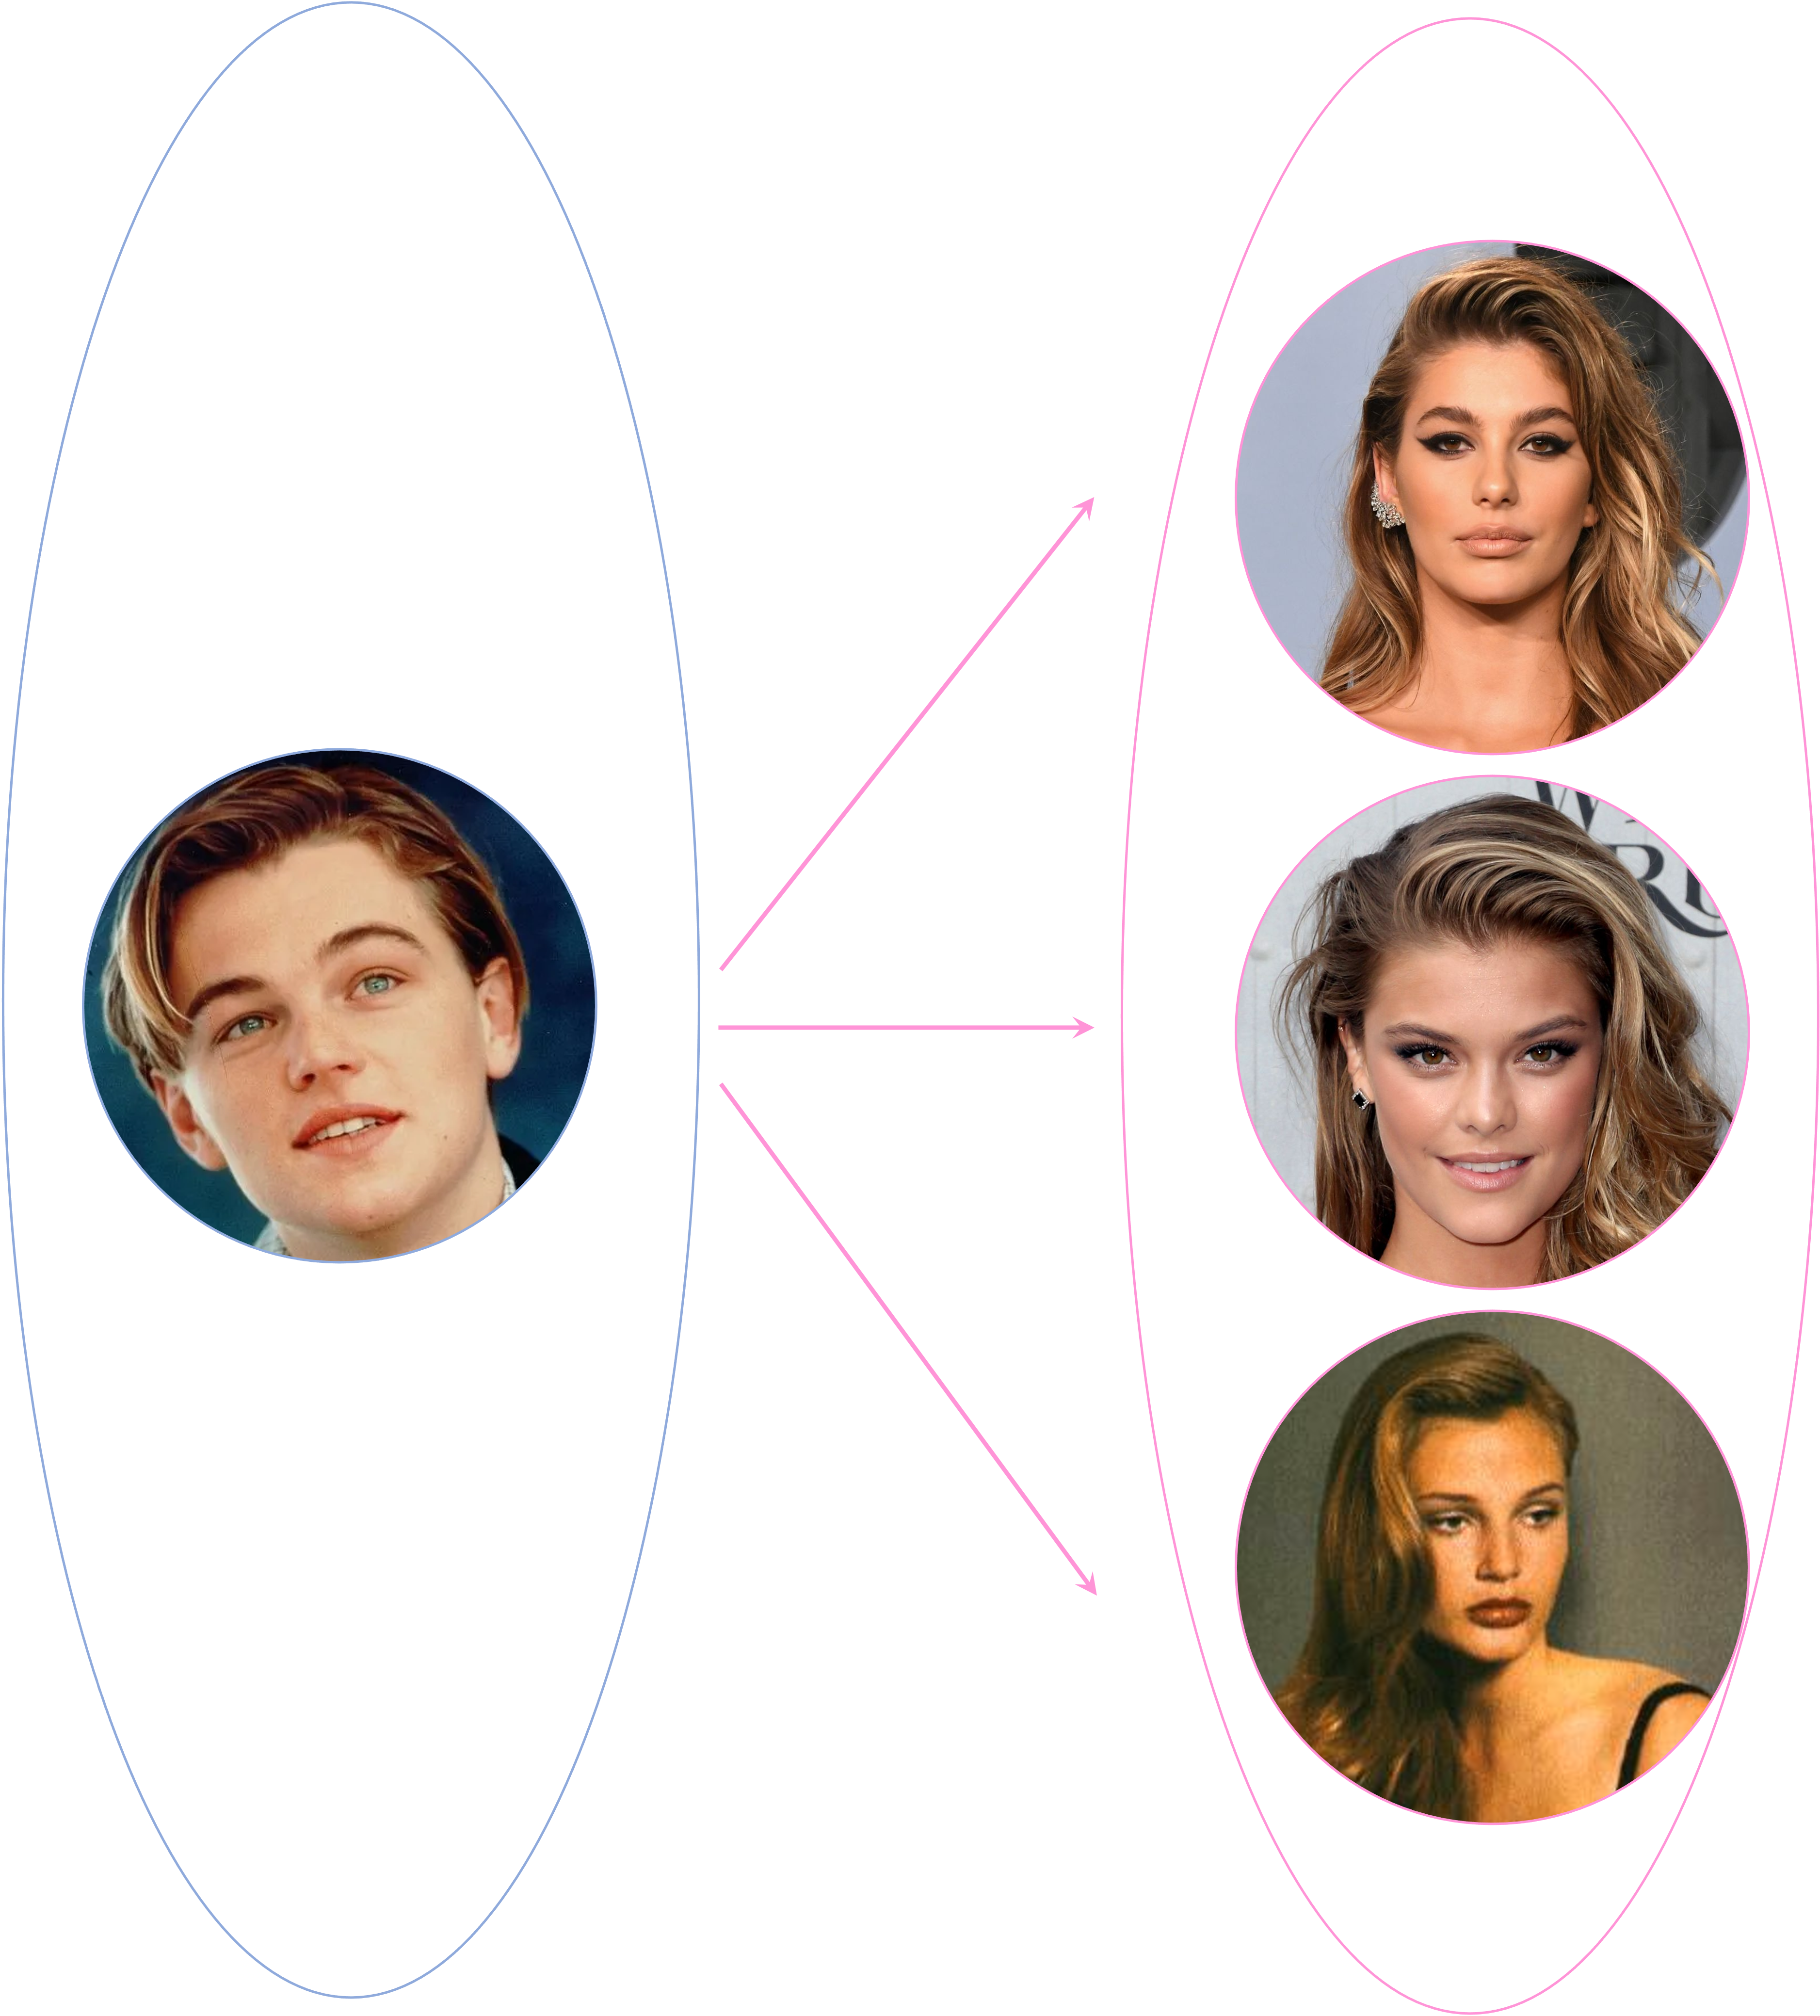
\includegraphics[width=0.5\textwidth]{Leonardo}
\caption{粗略统计Leonardo交往过20个女生}
\end{figure}

这也是一种映射,但是,左侧的一个元素对应着右侧多个元素。这种映射就是一对多的映射。

\subsection*{函数}
\label{subsec:Function}
上图的关系一对一关系就可以称之为是一种函数的。如果让$x$代表左边集合中的任意元素,$y$代表右边集合中的某一元素。那么我们就可以将这种函数关系记作如下的形式:
\[
	f: x\mapsto y  \qquad \text{or} \qquad  y=f(x)
\]
比如,上图当中的妻夫关系就可以计作$f(\text{高圆圆})=\text{赵又廷}$。但是很明显这样的表达式并不适合$f(\text{Leonard})$,等于号后面,填谁都不适合。因为这不是one-one relationship。

\subsubsection*{定义域与值域}
\label{Domain and Range}
当我们开始讨论数字集合的时候,集合中的元素开始变成数字的之后。$x$被我们称之为\gls{zbl},$y$称之为\gls{ybl}都是来自于两个数字集合的元素。在描述函数的时候,需要我们描述一下这两个集合的范围,其中$x$的范围被我们称之为\gls{domain}, $y$的范围被我们称之为\gls{range}。不过由于数字的运算特性,我们一般选择描述定义域就可以。可以通过函数的表达式确定出值域的大小。当然,考试的时候必定两个是可以互相求算的。

比如对于一个简单的二次函数:
\[
	y = x^2
\]
在这里不加任何限制的话,$x$可以选择带入任意实数数值,因此定义域为$x\in \mathcal{R}$。但是值域的话, $y$必定是非负数,因此值域可以计作$y\in [0,\infty)$。

但是如果考虑场景的话,比如$x$代表一个正方形的边长,$y$代表该正方形的面积。那么此时$x$作为一个长度就不能取到负值,并且边长为$0$的正方形也没太大意义。因此此时$x>0$就是这个函数的定义域了。
\clearpage


\section{反函数}
\label{sec:Inverse Function}
当我们考虑将左右侧的集合调换。形成如下图的映射:
\begin{figure}[H]
\centering
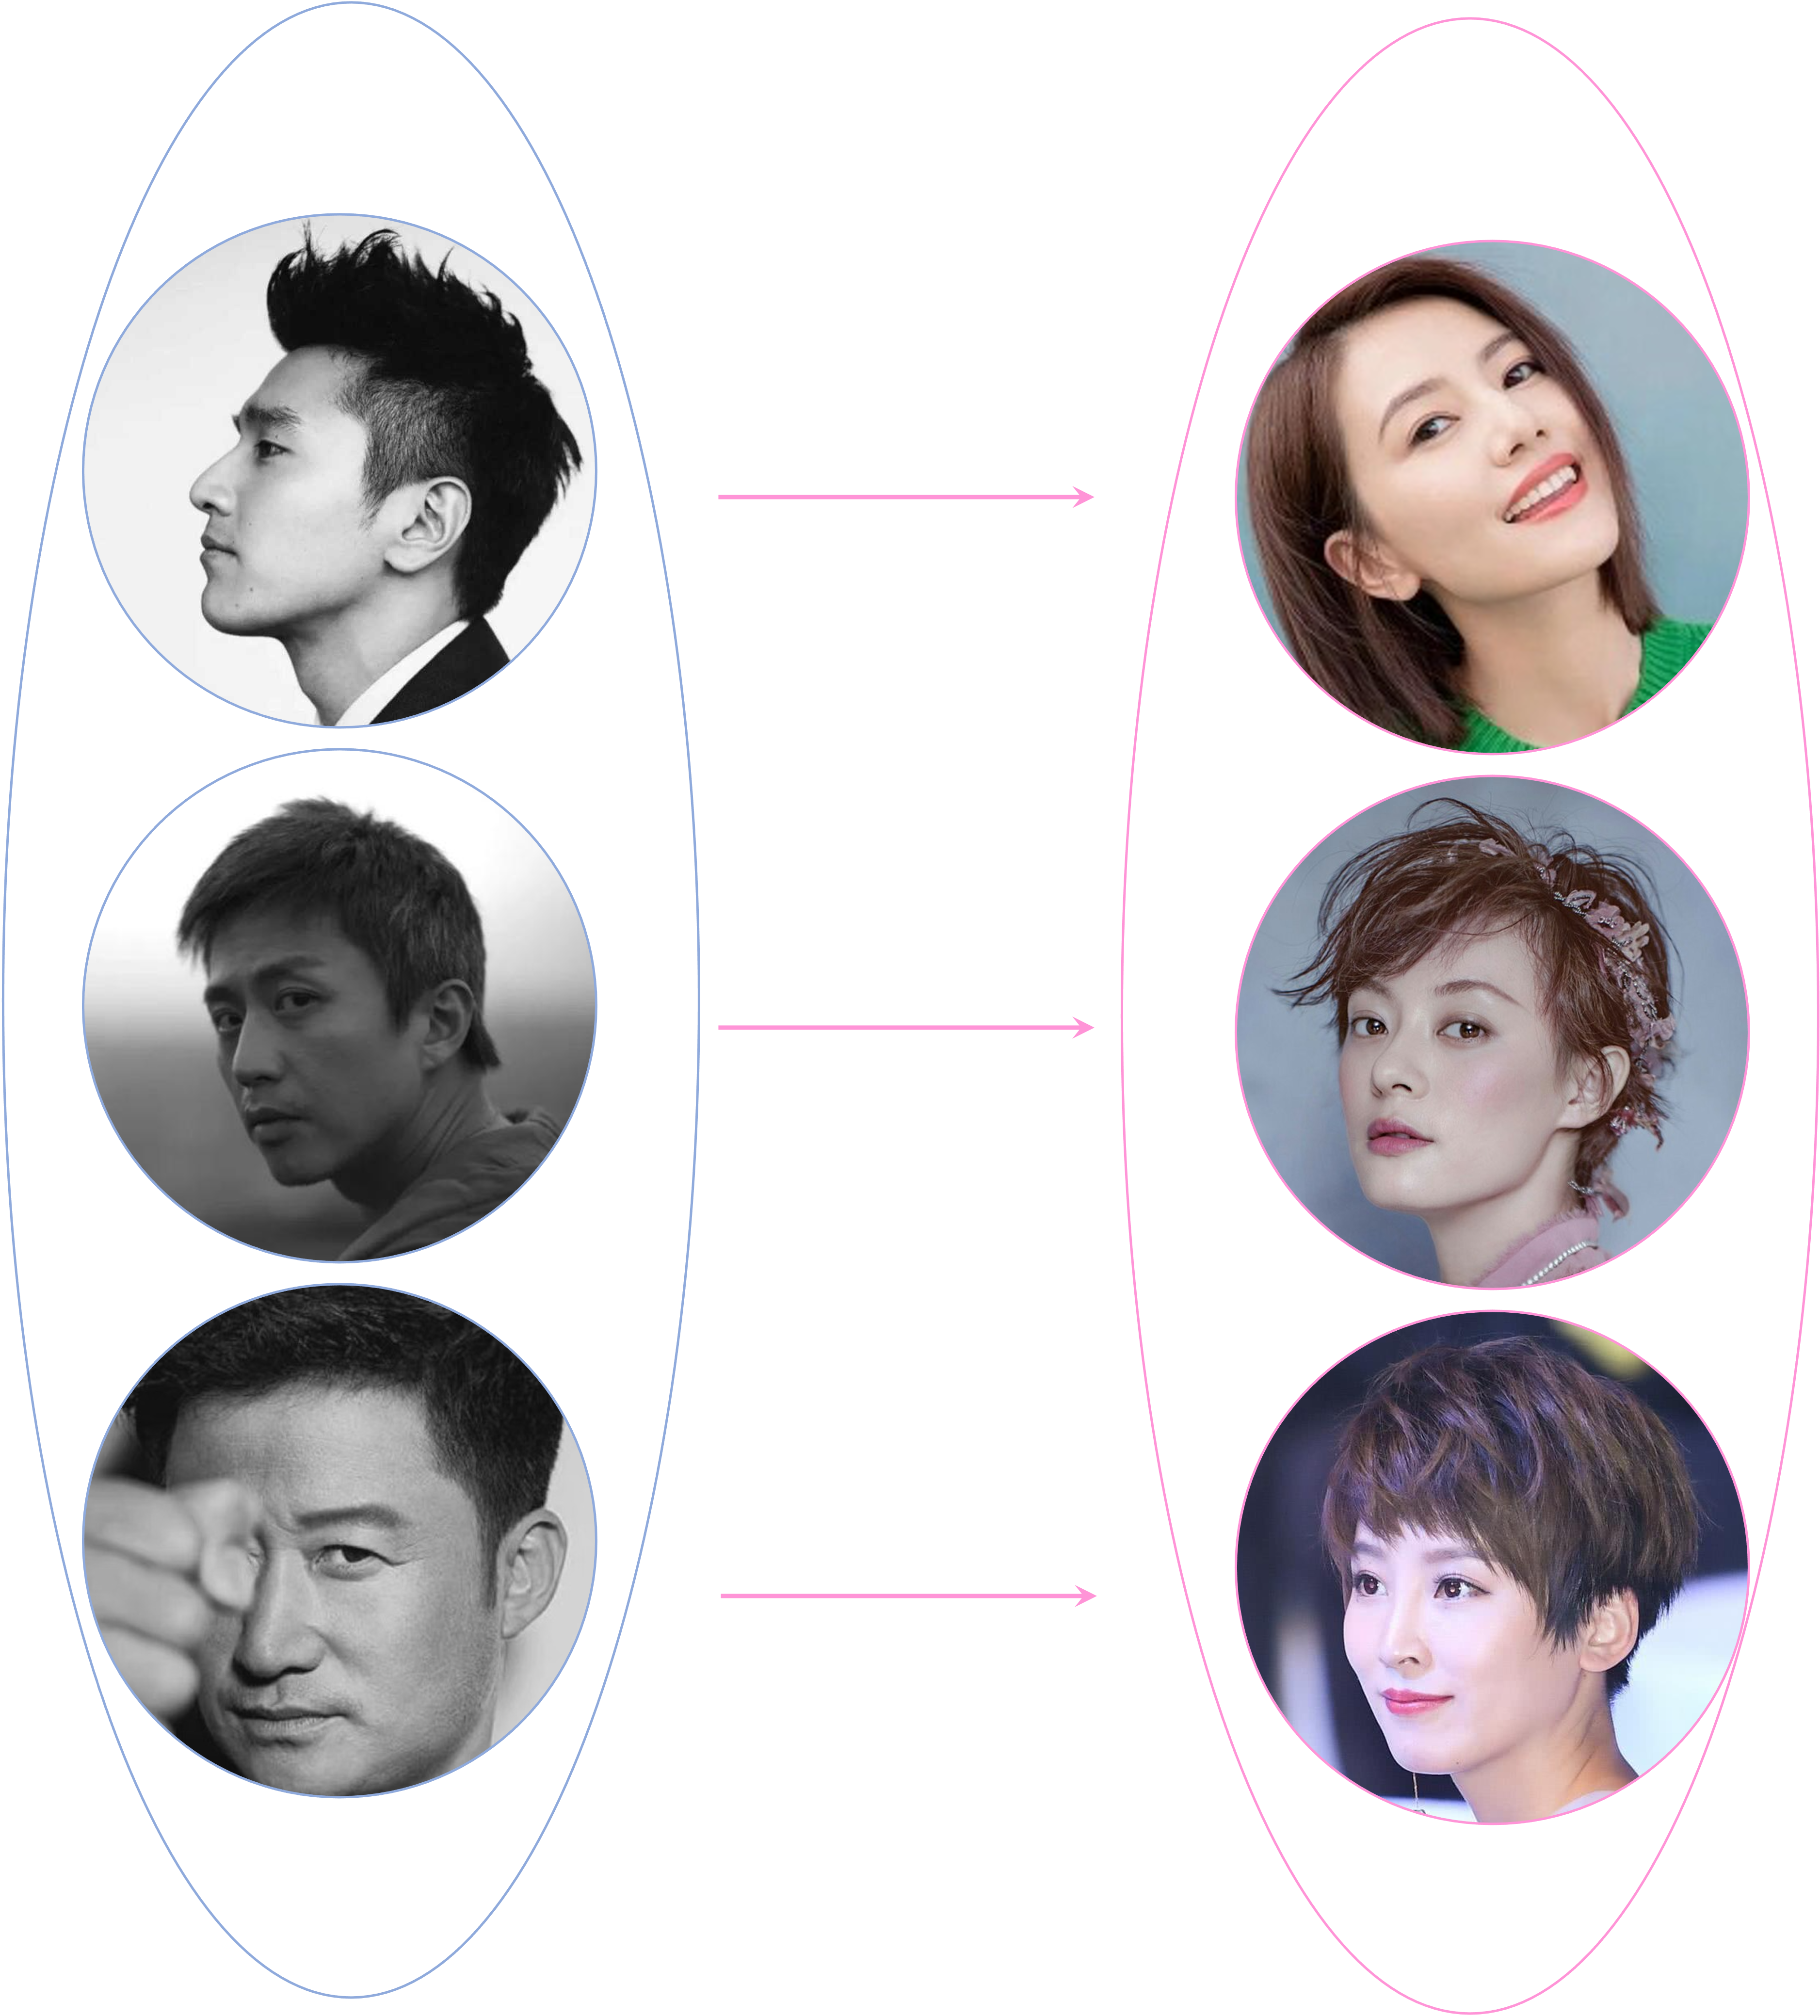
\includegraphics[width=0.5\textwidth]{husband-wife}
\caption{娱乐圈中的夫妻关系}
\end{figure}


赵又廷$\mapsto$高圆圆,邓超$\mapsto$ 孙俪, etc这些映射也是一对一的。因此必定也可以写作一个函数,之前已经确定了一个函数$f$,可以称之为找老公函数,那么这里就是它的\gls{inverse}。我们可以计作$f^{-1}$。当然如果不拘泥于这种写法的话,其实符号是可以任意选择的。比如$y=zlg(x)$ vs $y=zlp(x)$。只不过虽然这里两个函数的自变量都是$x$,但是取值的范围是完全不同的, 在$zlg$函数中,$x$的定义域是女生集合;但是在他的反函数$zlp$中,$x$的定义域是男生集合,恰好是原函数$zlg$中的值域。

\subsection*{能形成反函数的要求}
\label{subsec:Requirements}
由于反函数将原函数的值域作为自己的定义域。对于原函数,我们能确保,$x$只能对应一个$y$。但是对调之后这种关系可能不存在的了,如下面的函数
$h: x\mapsto (2x-3)^2-4$。当$x=1$或者$x=2$时,都对应着同样的$y=-3$。因此$h^{-1}(-3)$则陷入了和小李子一样的困境。不能满足one-one的要求,该函数则没有反函数。

\begin{SummBox}
能形成反函数,要求一个$x$有且只有一个$y$与之对应,与此同时,一个$y$值也只对应着一个$x$。
\end{SummBox}

\subsection*{确定反函数}
\label{subsec:Find Inverse}
对于上面的函数$y=h(x)=(2x-3)^2-4$,当我们把定义域稍作修改,从$x\in \mathcal{R}$ 改编成为$x>\frac{3}{2}$时,会满足了反函数存在的要求,因此就会有反函数存在了。那么如何确定这个反函数呢?

之前我们讨论过了,反函数交换了自变量和因变量。因此原函数的$x$现在成为了反函数中的$y$。原函数的$y$现在成为了反函数中的$x$。
比如$h(2)=-3$,那么$h^{-1}(-3)=2$。所以求算反函数只需要将表达式中的$x$,$y$对调一下就行了。
\[x=h(y)=(2y-3)^2-4\]
但是,我们希望得到的是$y=h^{-1}(x)$。因此需要再做一下整理化简:
\begin{align*}
x=h(y) &= (2y-3)^2-4\\
 x+4   &=(2y-3)^2\\
  2y-3 &=\sqrt {x+4} \quad \text{neglect negative value}\\
  y    &=\frac{\sqrt{x+4}+3}{2}\\
  y=h^{-1}(x) &=\frac{\sqrt{x+4}+3}{2}
\end{align*}

再陈述一下反函数$y=h^{-1}(x)$的定义域,$x>-4$就可以了

\begin{TaskBox}
$x>-4$是从哪里推导的?
\end{TaskBox}

\subsubsection*{反函数的图像特征}
\label{subsec:Graphic Charcteristic}
由于原函数和反函数的对应关系,最终会形成关于直线$y=x$对称的特征,并且如果原函数和反函数图像有交点的话,交点也只能在$y=x$图像上,思考一下为什么。

如下图所示,红线和蓝线就是两个互为反函数的图像。
\begin{figure}[H]
\centering
\includegraphics[width=0.8\textwidth]{inverse} %todo 原函数和反函数的图像
\caption{原函数和反函数的图像}
\end{figure}
\clearpage

\section{复合函数}
\label{sec:Composite Function}
\gls{comp}是将两个函数合并起来的函数。
比如:
\[f(x)=3x+2 \qquad g(x)=x^2+2x+4\]
那么: $fg(x)$则表示,将$x$首先带入到$g$函数中,然后再将得到的结果$g(x)$,代入到$f$函数中。等价于$f(g(x))=3\cdot g(x)+2$。

因此最后$fg(x)=3\cdot(x^2+2x+4)+2=3x^2+6x+14$。
在求算过程中需要注意,由于第一步要进行$g$函数的运算,因此$x$必须满足$g$的定义域;然后$g(x)$作为函数$f$的自变量,因此要满足$f$的定义域。这个点往往会被忽略掉。
\clearpage


\section{函数图像的变形}
\label{sec:Transformation of graphs}
当对一个函数进行简单的变形之后,也会对其图像产生一些变化。这些变化主要分为三大类。

\subsection*{平移}
\label{subsec:Translation}
对于一个函数$y=f(x)$而言,如果在原函数的基础上,改写为$y=f(x)+a$,构成一个新函数,那么这个新函数的图像会和原来的函数形状一模一样。只不过会从原函数的图像向\emph{上}\gls{py}$a$个单位(如果$a>0$)。向\emph{下}平移$a$个单位(如果$a<0$)。

原因如下:
假设$A$点的坐标为$(x_0,y_0)$,且满足$y_0=f(x_0)$,那么$A$点在原函数$y=f(x)$的图像上;假设$A'$点的横坐标与$A$点横坐标一致,且在$y=f(x)+a$上,那么$A'$点的坐标必定为$(x_0,y_0+a)$。也就意味着,$A'$点在竖直方向上与$A$点相差$a$个单位,如下图所示:
\begin{figure}[H]
\centering
\includegraphics[width=0.8\textwidth]{upshift.png}
\caption{图像在竖直方向上的平移}
\end{figure}

因此在一个函数表达式的最后加上或者减去某个数字带来的平行移动被我们称之为\emph{上加下减}。

但是接下来的概念会让很多人摸不着头脑,和之前相反。在水平方向上发生移动的规则被我们总结为\emph{左加右减}。也就是,如果$y=f(x+a)$这样的表达式会使新函数的图像出现在原函数的左边。

我们再重复刚才的一遍过程:
假设$A$点的坐标为$(x_0,y_0)$,且满足$y_0=f(x_0)$,那么$A$点在原函数$y=f(x)$的图像上;假设$A'$点的纵坐标与$A$点\emph{纵}坐标一致,且在$y=f(x+a)$上,那么此时,$A'$的横坐标求算要根据$y_0=f(x_0)$进行反推。由于$A'$是在新函数$y=f(x+a)$上的,因此可以写出:
\begin{align*}
y_0 &= f(x_0) \qquad \text{这是}A\text{点满足的关系}\\
y_0 &= f(x+a) \qquad \text{这是}A'\text{点满足的关系}\\
\end{align*}
对比之后,不难发现,$A'$点的横坐标等于$x_0-a$。而不像上下平移那样。因此$A'(x_0-a,y_0)$出现在$A(x_0,y_0)$的左侧(如果$a>0$),同理,整个新函数的图像会是原函数的图像向左边平移$a$个单位得到的。

\begin{figure}[H]
\centering
\includegraphics[width=0.8\textwidth]{leftshift}
\caption{图像在水平方向上的平移}
\end{figure}

\begin{SummBox}
左加右减,上加下减

$y=f(x+a)$ vs $y=f(x)+a$
\end{SummBox}


\subsection*{翻折}
\label{subsec:Reflection}
在这一小节中,我们将处理$y=-f(x)$与$y=f(-x)$的图像变形,这种结果是统称为翻折。

再次利用$A$与$A'$点的对应关系,对于$y=-f(x)$函数。$A(x_0,y_0)$在原函数上,那么当$A'$与$A$有一样的横坐标时,其纵坐标必定为$-f(x_0)=-y_0$。因此$A'$点与$A$点的关系是,横坐标相同,纵坐标互为相反数,当这种关系放在任意点上的时候,就能够使新函数与原函数的图像关于$x$轴对称,如下图所示
\begin{figure}[H]
\centering
\includegraphics[width=0.8\textwidth]{x-reflect}
\caption{沿$x$轴翻折的图像}
\end{figure}

同理,如果是$y=f(-x)$,由于此时是对$x$进行变形,因此$A'$点与$A$的关系是横坐标互为相反数,纵坐标相同,因此新函数与原函数的图像关于$y$轴对称,如下图所示
\begin{figure}[H]
\centering
\includegraphics[width=0.8\textwidth]{y-reflect}
\caption{沿$y$轴翻折的图像}
\end{figure}

\begin{SummBox}
$-f(x)$会使图像沿着$x$轴翻折;

$f(-x)$会使图像沿着$y$轴翻折。
\end{SummBox}

\begin{TaskBox}
如果是$-f(-x)$,新图像会发生什么样的变化
\end{TaskBox}

\subsection*{拉伸}
\label{subsec:Stretch}
这是考试当中最后一个函数图像的变形。$y=a\cdot f(x)$和$y=f(a\cdot x)$

还是一样,先看容易的。对整体表达式$f(x)$乘以$a$的运算操作。召唤老朋友$A(x_0,y_0)$和$A'$。由于$A'$的横坐标和$A$的横坐标一致,因此其纵坐标为$a\cdot f(x_0)=a\cdot y_0$刚好是$A$点坐标的$a$倍。而这样的结果是使得函数图像拉长(如果$a>1$),使得函数图像压扁(如果$0<a<1$)。就像膨胀或者缩小的气球一样。
\begin{figure}[H]
\centering
\includegraphics[width=0.8\textwidth]{expandingballoon}
\caption{绘制在气球上的函数图像会被拉伸}
\end{figure}

当然,上面图是帮助理解,下面的这张图才是真正Stretch by a factor greater than 1 or less than 1的图像:
\begin{figure}[H]
\centering
\includegraphics[width=0.4\textwidth]{stretch-v}
\includegraphics[width=0.4\textwidth]{compress-v}
\caption{竖直方向上的拉伸与压缩} %有可能会报错
\end{figure}


第二种,在水平方向上的拉伸与压缩,要靠$y=f(ax)$进行实现。召唤老朋友$A(x_0,y_0)$和$A'$。由于$A'$点和$A$点的\emph{纵}坐标保持一致。于是得到:
\begin{align*}
y_0 &= f(x_0) \qquad \text{这是}A\text{点满足的关系}\\
y_0 &= f(a\cdot x) \qquad \text{这是}A'\text{点满足的关系}\\
\end{align*}

那么显然$A'$的横坐标只能是$\frac{x_0}{a}$。因此新的对应点$A'(\frac{x_0}{a}, y_0)$会与原始点保持纵坐标相同,横坐标被压缩(如果$a>1$)或者拉伸(如果$0<a<1$)。其结论还是和竖直方向上的结论相反。
\begin{figure}[H]
\centering
\includegraphics[width=0.4\textwidth]{stretch-h}
\includegraphics[width=0.4\textwidth]{compress-h}
\caption{水平方向上的拉伸与压缩} %有可能会报错
\end{figure}

\begin{SummBox}
$y=af(x)$会使图像在\emph{竖直}方向上进行拉伸,如果$a>1$,图像会被拉长$a$倍;如果$0<a<1$则会使图像压缩$\frac{1}{a}$倍;

$y=f(ax)$会使图像在\emph{水平}方向上进行拉伸,如果$a>1$,图像会被压缩$a$倍;如果$0<a<1$则会使图像拉长$\frac{1}{a}$倍;
\end{SummBox}


\subsection*{变形的结合}
\label{subsec:Combination of Transformation}
考试不会如此仁慈地只讨论一种变形,在表达式中常常会将多种变形结合在一起,重要的是能够确定执行那些操作,以及这些操作的量。

比如

1. $y=-3f(x)$ 

明显就是可以先操作$y=3f(x)$,也就是竖直方向上拉伸$3$倍,再执行关于$x$轴的翻折

2. $y=f(2x+4)$

方法1:\\
先进行平移的向左边移动$4$个单位得到$y=f(x+4)$;再进行水平方向上的压缩,$2$倍;

方法2:\\
先进行水平方向上的压缩,$2$倍得到$y=f(2x)$;注意,此时无需再向左边移动$4$个单位,而是仅仅移动$2$个单位。原因是:此时$x$作为整体,当向左平移$2$个单位的时候,表达式变成$y=f(2\boxed{(x+2)})=f(2x+4)$。因此如果使用先拉伸压缩,再平移量的方法,平移量会受到系数的影响。需要牢记。

在该\href{https://www.desmos.com/calculator/6yzdqimnlc}{Shift and Transformation}中有所有三种变形的情况,多调整一下滑块
体会一下这三种变动。





\chapter{坐标几何}
\label{ch:Coordinate Geometry}
坐标几何学是代数学和几何学两者共同孕育出来的儿子。
当笛卡尔发明了坐标轴系统之后,几何学中的平面上的点,可以用两个坐标轴的数值进行确定;几何学中的直线与线性函数的的图像就变成了同一个事物,可以用含有$x$,$y$的代数式进行表示。于是坐标几何学就诞生了。

也成为了现在\href{https://www.autodesk.com}{AutoCad},Blender,\href{https://www.geogebra.org}{Geogebra}这些软件的基石。

\section*{学习目标}
\begin{todolist}
 \item 根据已知信息求算直线的表达式
 \item 掌握表示直线的几种形式,包括\gls{xjs},\gls{dxs}以及\gls{ybs}
 \item 理解并运用\gls{bzfc}
 \item 利用代数运算求解直线和圆有关的问题
 \item 理解任意图形与其代数表达式的等价关系
 \item 利用图像的交点求算方程的解
\end{todolist}
\clearpage

\section{直线}
\label{sec:Straight Line}
直线是除了点之外,最简单的几何图形,直线的表达式必定可以用
\[
	y=mx+c
\]
进行表示的。而且由于两点确定一条直线,因此求算坐标系中直线的表达式仅需要提供两个点就可以了。\gls{slope}的求算通过:
\[
	m=\frac{y_2-y_1}{x_2-x_1}
\]

\gls{jj}则可以带入到任何一个点的横纵坐标,进而确定。

\begin{TaskBox}
Find the slope-intercept form a line passnig through the point $(2,5)$ and $(3,4)$.
\end{TaskBox}

\subsection*{点斜式}
\label{subsec:Point Slope Form}
如果给定的信息是斜率和一个点的坐标的话,其实我们有更加简洁的方式去定义这条线。比如在上一条Task当中,该直线的斜率为$-1$,如果再已知该直线通过一个点$(3,4)$的话,利用斜率的定义:
\begin{align}
 \notag m=-1 &=\frac{y-4}{x-3}\\ %编号和引用参考的问题
  y-4 &=-1(x-3)
\end{align}

将直线所通过的点的横纵坐标,以及该直线的斜率全部表述出来的形式被称之为\gls{dxs}。具有如下的形式:
\[
	y-y_0 = m(x-x_0)
\]
其中,$m$是斜率,$(x_0,y_0)$是直线当中某一个点的具体坐标。

\begin{TaskBox}
思考,$y=m(x)+c$ 如何修改为点斜式,使其通过的点为$y$轴截距
\end{TaskBox}


\subsection*{普通式}
\label{subsec:Standard Form of a line}
在之前的两种形式中,需要某一条直线具有特定的斜率。但是,当一条完全垂直于$x$轴的直线式,无论如何,都无法用上面的两种形式进行表示。因为这样的线是没有斜率的,或者说斜率是underfined。为了能够囊括所有的直线。我们把$x$,$y$都移动到同一侧,得到如下的直线的形式:
\[
	ax+by=c \qquad ax+by+c=0
\]
在这样的表达式中,斜率并没有直接体现出来。但是,这种表达式的好处在于,$x$和$y$之前的系数可以为0。包含了完全水平的直线$by=c$,或者完全垂直的直线$ax=c$,这两种额外的形式。

\begin{TaskBox}
将$y=-x+7$整理为普通式
\end{TaskBox}
\clearpage


\section{圆的标准方程}
\label{sec:Standard Equation of a Cricle}
回顾一下两点间的距离公式:
\[
	d=\sqrt{(x_2-x_1)^2+(y_2-y_1)^2}
\]

再回顾一下圆的定义:\\
到固定点的长度等于固定值的所有的点所形成的几何图形。该固定点称之为圆心,该固定值长度称之为\gls{radius}。

于是,在一个坐标系中,假设$(x,y)$是圆上任意一点,$(a,b)$为圆心,$r$为该圆的半径。那么$x$,$y$必定满足如下的方程
\[
	(x-a)^2+(y-b)^2=r^2
\]
形如这样的表达式的方程被称为\gls{bzfc}。在这种表达式下,圆心坐标和半径就被清楚地罗列出来了。

\begin{figure}[H]
\centering
\includegraphics[width=0.8\textwidth]{rainbow}
\caption{彩虹就是标准的圆形}
\end{figure}

打开该\href{https://www.desmos.com/calculator/nasxcwsa73}{Desmos}演示,查看一道美丽的正圆彩虹。

\begin{TaskBox}
为什么这里不称之为圆的函数,而只能叫做圆的方程?
\end{TaskBox}

\subsection*{圆的一般方程}
\label{subsec:Normal Equation of a circle}
当然,由于二次平方的展开,圆的标准方程也可以展开为普通方程:
\begin{align*}
	(x-a)^2+(y-b)^2 &=r^2\\
	x^2-2ax+a^2+y^2-2by+b^2 &=r^2\\
	x^2+y^2+Ax+By+C&=0
\end{align*}

所以这两者之间要能够互相转化。

\begin{TaskBox}
将$x^2+2x+y^2-4y-3=0$转变为圆的标准方程,并写出该圆的圆心坐标和半径。
\end{TaskBox}

\subsection*{点和圆的位置关系}
\label{subsec:Position of a Point with repsect to a Circle}
当一个点在圆内时,其到圆心的距离必定小于半径,因此沿用标准方程:
\[
	(x-h)^2+(y-k)<r^2
\]
就表示在圆内的所有点。

当一个点在圆外时,其到圆心的距离必定大于半径,继续沿用标准方程:
\[
	(x-h)^2+(y-k)>r^2
\]
就表示在圆外的所有点。
\clearpage


\section{直线与圆的联立}
\label{subsec:Line and Circle}
一条直线和圆会形成相交,相切,以及相离的位置关系。如下图所示:
\begin{figure}[H]
\centering
\includegraphics[width=0.8\textwidth]{lineCircle}
\caption{三种不同的圆和直线的关系}
\end{figure}

根据之前所学,由于直线和圆都具有代数表达式,因此将其对应的代数式进行联立得到如下的方程组:
\[
\left\{\begin{matrix}
y=mx+c\\
(x-a)^2+(y-b)^2=r^2
\end{matrix}\right.
\]
该表达式的解就是对应图像的交点。而解决该方程组的固定做法是:

\noindent1.利用$y$和$x$的线性关系,只保留一个变量\\
2.将圆的方程转变为关于$x$或者$y$的一元二次方程\\
3.求解该方程,并将结果带入到线性函数中。确定坐标。

\begin{TaskBox}
证明直线$y=-x+2\sqrt 2$与$x^2+y^2=4$相切,求算其切点
\end{TaskBox}
\clearpage


\chapter{弧度制}
\label{ch:Circular Measure}
现在你们要学习高级一点的角度表示方法了。就像小时候采用$1,2,3$这样的数字系统,到了高中之后采用$x,y,z$这样的代数系统。描述角度新的方法就是\gls{radians}
\begin{figure}[H]
\centering
\includegraphics[width=0.8\textwidth]{calc-radian}
\caption{TI-nspire当中角度度量的选择}
\end{figure}


\section*{学习目标}
\begin{todolist}
 \item 理解角度制和弧度制作为衡量一个角大小的测度系统
 \item 记忆和运用弧度制的定义和相关公式
 \item 对一个角的弧度制和角度制结果实现互相转化
 \item 利用弧度制求算扇形的弧长以及面积,解决其他相关问题
\end{todolist}
\clearpage


\section{弧度}
\label{sec:Radian}
我们之前定义$1$\si{\degree}的角是通过:将一个\gls{pangle}做180等分,每一份的角就是$1$\si{\degree}。因此在这种角度制的体系下,角的大小是携带有``\si{\degree}''这样的单位的。

而现在新的体系下,我们将角放入到扇形当中,用扇形的弧长和半径之比作为该角的大小。
\begin{figure}[H]
\centering
\includegraphics[width=0.8\textwidth]{DegRad} 
\caption{度数制系统和弧度制系统}
\end{figure}

因此我们定义一个角的弧度制的定义是:
\[
	\theta=\frac{\ell}{r}
\]

\subsection*{弧度制与度数制的转换关系}
\label{subsec: Convertion between Radians and Degrees}
根据定义,一个$180$\si{\degree}的角,安置在扇形中,其弧长为$\frac{1}{2}\cdot 2\pi r$。因此平角的弧度为$\frac{\frac{1}{2}\cdot 2\pi r}{r}=\pi$。这就是我们对弧度制和度数制的基本转换关系:
\[
	180\si{\degree} = \pi \text{ rad} \approx 3.141592 \text{ rad}
\]
因此任意任意角度$n$\si{\degree}都可以转化为对应的弧度$\theta$。转化公式如下:

\begin{align*}
	\theta &=\frac{\frac{n \si{\degree}}{360\si{\degree}}\cdot 2\pi r}{r} \\
			&=\frac{n \si{\degree}}{360\si{\degree}}\cdot 2\pi\\
			&=\frac{n \si{\degree}}{180\si{\degree}}\cdot \pi\\
			&=n\si{\degree} \cdot \frac{\pi}{180\si{\degree}}
\end{align*}

那么,如果将弧度制的角转变为度数制的角的话,则是一个相反的逆过程:
\[
	n\si{\degree} =\theta \cdot \frac{180\si{\degree}}{\pi}
\]

由此,稍微记牢一下常见的特殊角对应的角度制和弧度制数值。
\begin{table}[H]
\centering
\begin{tblr}{
	colspec={|l|[2pt,dotted]c|c|c|c|c|c|c|c|c|c|},
	hspan=0.7\textwidth
	}
\hline
Deg & 0\si{\degree} & 30\si{\degree} & 45\si{\degree} & 60\si{\degree} & 90\si{\degree} & 120\si{\degree} & 150\si{\degree} & 180\si{\degree} & 270\si{\degree} & 360\si{\degree} \\ 
\hline 
Rad & 0 & $\quad$ & $\quad$ & $\quad$ & $\quad$ &$\quad$ & $\quad$& $\pi$&$\quad$  & $2\pi$\\ 
\hline
\end{tblr}
\end{table}


\begin{TaskBox}
完成表格当中空余的部分
\tcblower 
思考这些表格中的$\pi$是不是弧度制的单位?或者说弧度制有没有单位?
\end{TaskBox}
\clearpage


\section{扇形性质}
\label{sec:Property of Sector}
对于一个扇形,当已知该扇形的圆心角(以弧度制记)和半径之后,其弧长的求算公式为:
\[
	\ell =r\cdot \theta
\]
而对于其面积,求算公式为:
\begin{align*}
	A &= \frac{\theta}{2\pi} \cdot \pi r^2 \\
		&=\frac{1}{2} r^2\theta\\
		&=\frac{1}{2}r \cdot \ell
\end{align*}
而如果是扇形的弦长的话,其长度的求算公式则为:
\[
	\text{chord length} =2r\cdot \sin \left(\frac{\theta}{2}\right)
\]

如下图所示,所有的求算结果都标记出来的
\begin{figure}[H]
\centering
\includegraphics[width=0.8\textwidth]{sector}
\caption{扇形中的各种求算}
\end{figure}


\clearpage


\chapter{三角学}
\label{ch:Trigonometry}
还是一样,和IGCSE阶段相比,在Alevel阶段我们将了解更多关于三角比的以及三角函数的内容

\section*{学习目标}
\begin{todolist}
	\item 牢记并应用特殊角的正弦值,余弦值,正切值。以及相关变化
	\item 牢记并运用三角恒等式
	\item 求算给定区间区间内的含有三角比的方程
	\item 理解单位圆的作用
	\item 绘制$\sin$,$\cos$,$\tan$的函数图像,包括改变振幅,周期,初相位等变化
	\item 理解反三角函数可以用来求算角的大小
\end{todolist}
\clearpage

\section{三角比}
\label{sec:Trigonometric Ratio}
回顾一下三角比的定义 SOH CAH TOA\footnote{Opposite, Adjacement, Hypotenuse的缩写,sine,cosine和tangent的缩写}。

\subsection*{特殊角的三角比}
\label{subsec:Special Angle}
结合两个特殊三角形。可以完成以下的表格
\begin{figure}[H]
\centering
\includegraphics[width=0.8\textwidth]{SpecialTriangle}
\caption{两个特殊三角形以及边长}
\end{figure}

\begin{table}[H]
\centering
\begin{tblr}{|l|c|c|c|}
\hline
$\theta$ & $\frac{\pi}{6}$ & $\frac{\pi}{4}$ & $\frac{\pi}{3}$\\
\hline
$\sin\theta$ &$\frac{1}{2}$& & \\
\hline
$\cos\theta$ & & $\frac{\sqrt2}{2}$& \\
\hline
$\tan\theta$ & $\frac{\sqrt3}{3}$ & & \\
\hline
\end{tblr}
\end{table}

\begin{TaskBox}
完成上方表格当中剩余的空白处
\end{TaskBox}


\subsection*{单位圆}
\label{subsec:Unit Circle}
当我们引入半径为$1$,圆心在原点的圆的时候,构造任意的半径旋转的角度$\theta$就可以用旋转点的\emph{横}
/\emph{纵}坐标来代替该角度$\theta$的正余弦值,以及求算正切值。如下图:

\begin{figure}[H]
\centering
\includegraphics[width=0.8\textwidth]{unitcircle}
\caption{单位圆用点的坐标表示一个角度的$\sin$,$\cos$值}
\end{figure}

\begin{TaskBox}
补齐单位圆上剩余的特殊点的坐标,以及确定对应角度的正弦,余弦,正切值。
\end{TaskBox}

\subsection*{三角恒等式}
\label{subsec:Trig Identity}
根据单位圆上或者其他的证明,有以下的恒等关系始终存在,这些恒等关系需要牢记并进行运用
\begin{align}
\sin^2\theta+\cos^2\theta &= 1\\
\sin(\frac{\pi}{2}-\theta) &= \cos \theta \\
\tan \theta =\frac{\sin \theta}{\cos \theta}
\end{align}

\begin{TaskBox}
已知某角度$\theta$的$\tan$值为3;求算$\sin \theta$ 和$\cos \theta$。
\end{TaskBox}
\clearpage


\section{三角函数}
\label{sec:Unit Circle and Trigonometric Function}
由于单位圆的存在,我们在理解角度上的时候,再也不需要拘泥于度数制的限制,$\theta$角可以取任意的值,并且,由于负值的时候,仅需要把角度进行顺时针旋转即可。因此以角度$\theta$作为自变量$x$,以其三角比的值作为因变量$y$。构建如下的三种函数关系$y=\sin x$, $y=\cos x$, $y=\tan x$。逐一进行研究

\subsection*{正弦函数}
\label{subsec:Sine function}
我们将采用描点法绘制三种函数的图像,首先,结合单位圆,完成以下的表格:

\begin{table}[H] %这个表格的长宽设计的不太合理。
\centering
\begin{tblr}{
	colspec={|l|[2pt]c|c|c|c|c|c|c|c|c|},
	hspan=even, %设置一样长度
	vspan=even,
	}
\hline 
$x$(in rad) & 0 & $\frac{\pi}{6}$ & $\frac{\pi}{4}$ & $\frac{\pi}{3}$ & $\frac{\pi}{2}$ &$\frac{2\pi}{3}$ & $\frac{3\pi}{4}$&$\frac{5\pi}{6}$ &$\pi$\\
\hline
$y=\sin x$ &$\quad$ &$\quad$ &$\quad$ &$\quad$ &$\quad$ &$\quad$ &$\quad$ &$\quad$ \\
\hline
$x$(in rad)& $\frac{7\pi}{6}$ & $\frac{5\pi}{4}$ & $\frac{4\pi}{3}$& $\frac{3\pi}{2}$ & $\frac{10\pi}{6}$& $\frac{7\pi}{4}$& $\frac{11\pi}{6}$ &$2\pi$\\
\hline
$y=\sin x$ &$\quad$ &$\quad$ &$\quad$ &$\quad$ &$\quad$ &$\quad$ &$\quad$ &$\quad$ \\
\hline
\end{tblr}
\end{table}

\begin{TaskBox}
完成以上的表格
\tcblower
在下方的函数图像中选择对应的点
\end{TaskBox}

\begin{figure}[H]
\centering
\includegraphics[width=\textwidth]{sinefunc}
\caption{标准正弦函数图}
\end{figure}

因此就形成正弦函数的图像。请关注以下的几个点:
\begin{itemize}
	\item 函数最大值和最小值出现的地方
	\item 函数值为0的地方
	\item 该函数的周期性
	\item 该函数的对称性
\end{itemize}

\subsection*{余弦函数}
\label{subsec:Cosine Function}
一样的过程,再重复一遍。

\begin{table}[H]
\centering
\begin{tblr}{
	colspec={|l|[2pt]c|c|c|c|c|c|c|c|c|},
	hspan=even, %设置一样长度
	vspan=even,
	}
\hline 
$x$(in rad) & 0 & $\frac{\pi}{6}$ & $\frac{\pi}{4}$ & $\frac{\pi}{3}$ & $\frac{\pi}{2}$ &$\frac{2\pi}{3}$ & $\frac{3\pi}{4}$&$\frac{5\pi}{6}$ &$\pi$\\
\hline
$y=\cos x$ &$\quad$ &$\quad$ &$\quad$ &$\quad$ &$\quad$ &$\quad$ &$\quad$ &$\quad$ \\
\hline
$x$(in rad)& $\frac{7\pi}{6}$ & $\frac{5\pi}{4}$ & $\frac{4\pi}{3}$& $\frac{3\pi}{2}$ & $\frac{10\pi}{6}$& $\frac{7\pi}{4}$& $\frac{11\pi}{6}$ &$2\pi$\\
\hline
$y=\cos x$ &$\quad$ &$\quad$ &$\quad$ &$\quad$ &$\quad$ &$\quad$ &$\quad$ &$\quad$ \\
\hline
\end{tblr}
\end{table}

绘制的函数图如下:
\begin{figure}[H]
\centering
\includegraphics[width=\textwidth]{cosinefunc}
\caption{标准余弦函数图}
\end{figure}

\begin{TaskBox}
根据描点,绘制$y=cos(x)$的函数图像,并且绘制小于0,以及大于$2\pi$时的图像。
\end{TaskBox}

与正弦函数一样,请描述这个图像的一下几个方面:
\begin{itemize}
	\item 函数最大值和最小值出现的地方
	\item 函数值为0的地方
	\item 该函数的周期性
	\item 该函数的对称性
\end{itemize}


\subsection*{正切函数}
\label{subsec:Tangent Function}
根据$\tan x =\frac{\sin x}{\cos x}$。完成以下的表格的绘制:

\begin{table}[H]
\centering
\begin{tblr}{
	colspec={|l|[2pt]c|c|c|c|c|c|c|c|c|},
	hspan=even, %设置一样长度
	vspan=even,
	}
\hline 
$x$(in rad) & 0 & $\frac{\pi}{6}$ & $\frac{\pi}{4}$ & $\frac{\pi}{3}$ & $\frac{\pi}{2}$ & $-\frac{\pi}{6}$ & -$\frac{\pi}{4}$ & -$\frac{\pi}{3}$ & -$\frac{\pi}{2}$\\
\hline
$y=\tan x$ &$\quad$ &$\quad$ &$\quad$ &$\quad$ &$\quad$ &$\quad$ &$\quad$ &$\quad$
\hline
\end{tblr}
\end{table}

因此该函数的图像如下图:
\begin{figure}[H]
\centering
\includegraphics[width=\textwidth]{tangfunc}
\caption{标准正切函数}
\end{figure}

\noindent 有两个点是额外值得关注的,\\
第一个是$y=\tan x$的周期此时不是$2\pi$。应该变成了多少?\\
第二个是\gls{asymptote}。由于$x$不能取得$\frac{\pi}{2}$以及其整倍数值,因此函数的图像不可能与$x=\frac{\pi}{2}$相交,只能无限地靠近该竖直直线,因此是有渐近线的。这是正切函数独有的

\begin{SummBox}
三种基础的三角函数图像分别如下图:
\begin{figure}[H]
\centering
\includegraphics[width=0.3\textwidth]{sinefunc-2}
\includegraphics[width=0.3\textwidth]{cosinefunc-2}
\includegraphics[width=0.3\textwidth]{tangfunc-2}
\end{figure}
需要牢记特殊点(5个)。
\end{SummBox}


\subsection*{非标准三角函数}
\label{subsec:Nonstandard Trigonometric Function}
回顾一下之前我们所说的函数的变形。这一小节的内容就是\emph{上加下减,左加右减}以及\emph{拉伸压缩}的具体应用。

因此,我们需要解决如下的几种变形,以及这三者之间的结合。最终实现绘制$y=A\sin (\omega x+\varphi)+C$的图像。

\subsubsection*{水平相位}
$y=\sin (x+\varphi)$会产生水平方向的移动。利用左加右减即可。
\begin{TaskBox}
在下图$y=\sin x$的函数图像中,绘制$y=\sin(x+\frac{\pi}{6})$ 以及 $y=\sin(x-\frac{\pi}{4})$的图像。
\begin{figure}[H]
\centering
\includegraphics[width=0.8\textwidth]{sinefunc-2}
\end{figure}

\end{TaskBox}


\subsubsection*{中间值的移动}
$y=\sin x +C$会产生竖直方向的移动。利用上加下减即可。
\begin{TaskBox}
在下图$y=\sin x$的函数图像中,绘制$y=\sin x+1$ 以及 $y=\sin x-2$的图像。
\begin{figure}[H]
\centering
\includegraphics[width=0.8\textwidth]{sinefunc-2}
\end{figure}
\end{TaskBox}

\subsubsection*{最值的拉伸与翻折}
$y=A\sin x$ 会使的图像发生拉伸变形\\
当$A>1$时,竖直方向上的拉长,会使得函数的最值从$\pm 1$变成 $A\cdot \pm 1=\pm A$;\\
当$0<A<1$时,则是将函数压扁。\\
如果$A$是负值,只需要在拉伸或者压缩之后再沿着$x$轴进行翻折即可。
、
\begin{TaskBox}
在下图$y=\sin x$的函数图像中,绘制$y=-3\sin x$ 以及 $y=\frac{1}{2}\sin x$的图像。
\begin{figure}[H]
\centering
\includegraphics[width=0.8\textwidth]{sinefunc-2}
\end{figure}
\end{TaskBox}

\subsubsection*{周期的变化}
$y=\sin(\omega x)$会产生水平方向的拉伸或者压缩。因此:\\
当$\omega>1$时,将整个图像做压缩,周期会变成$\frac{2\pi}{\omega}$\\
当$0<\omega<1$时,将整个图像做拉伸,周期会变成$\frac{2\pi}{\omega}$\\

\begin{TaskBox}
在下图$y=\sin x$的函数图像中,绘制$y=\sin (4x)$ 以及 $y=\sin (\frac{1}{2}x)$的图像。
\begin{figure}[H]
\centering
\includegraphics[width=0.8\textwidth]{sinefunc-2}
\end{figure}
\end{TaskBox}
\clearpage

\section{反三角}
\label{sec:Inverse Trig}
既然角度有对应的三角比值,那么根据三角比值也能反推角度。此时我们只需要利用\gls{inverse trig}

\subsection*{反三角函数的定义}
举例:$\sin \frac{\pi}{6}= \frac{1}{2}$。因此当已知一个角的sine值为$\frac{1}{2}$时,该角度可以通过$\sin^{-1} (\frac{1}{2})$或者$\arcsin \left( \frac{1}{2}\right)$确定
如下图所示
\begin{figure}[H]
\centering
\includegraphics[width=0.7\textwidth]{ioscalc}
\caption{iPhone上如何调出这个反三角函功能?}
\end{figure}

\subsection*{求解$\sin x=a$的结果}
利用刚才所说:
$x=\sin^{-1} a=\theta$。但是,如果我们将$x$的范围限制在$0\le x\le 2\pi$的话。这样的解会有两个,可以利用单位圆进行确定。
\begin{figure}[H]
\centering
\includegraphics[width=0.5\textwidth]{sina}
\caption{利用单位圆求解$\sin x=a$}
\end{figure}

因此,在一个周期的图像内,一般而言有两个角度的正弦值,可以等于同样的结果,两者之和为$\pi$ 或者 180\si{\degree}。 比如$\sin \frac{\pi}{6}=\sin \frac{5\pi}{6}=\frac{1}{2}$。


\subsection*{求解$\cos x=a$的结果}
和刚才一样。$x=\cos^{-1} a=\theta$。但是,如果我们将x的范围限制在$0\le x\le 2\pi$的话。这样的解也会有两个。
\begin{figure}[H]
\centering
\includegraphics[width=0.5\textwidth]{cosa}
\caption{利用单位圆求解$\cos x=a$}
\end{figure}
因此,在一个周期的图像内,一般而言有两个角度的余弦值,可以等于同样的值,两者之和为$2\pi$ 或者 $360$\si{\degree}。比如$\cos \frac{\pi}{3}=\cos \frac{5\pi}{3}=\frac{1}{2}$。


\subsection*{求解$\tan x=a$的结果}
和刚才一样。$x=\tan^{-1} a=\theta$。但是,如果我们将$x$的范围限制在$0\le x\le 2\pi$的话。这样的解也会有两个。

\begin{figure}[H]
\centering
\includegraphics[width=0.5\textwidth]{tana}
\caption{利用单位圆求解$\tan x=a$}
\end{figure}
因此,在两个周期的图像内,一般而言有两个角度的正切值,可以等于同样的值,两者之差为$\pi$ 或者 $180$\si{\degree}。比如$\tan \frac{\pi}{4}=\tan \frac{5\pi}{4}=1$。

\begin{SummBox}
1.如果两个角$\alpha$和$\beta$,满足$\alpha+\beta=\pi$,那么$\sin \alpha=\sin \beta$;\\
2.如果两个角$\alpha$和$\beta$,满足$\alpha+\beta=2\pi$,那么$\cos \alpha=\cos \beta$;\\
3.如果两个角$\alpha$和$\beta$,满足$\alpha-\beta=\pi$,那么$\tan \alpha=\tan \beta$;
\end{SummBox}

\begin{TaskBox}
以上的总结内容仅针对于$[0,2\pi)$,但是由于周期性的存在,两角相等的结果还有其他的结论。尝试推导,当$-\pi\le x\le \pi$时,$\alpha$和$\beta$需要满足什么条件才可以使其正弦值相等。
\end{TaskBox}

\clearpage

\section{含有三角函数的方程}
\label{sec:Equation with Trig}
现在开始处理含有的三角比的方程。
\begin{ExampleBox}
$3\sin(2x)+1 =0$ for $-\pi\le x\le \pi$\\

Solution:
\begin{align*}
\sin (2x) &= -\frac{1}{3}\\
		2x &=\sin^{-1}\left(-\frac{1}{3}\right)\\
		   &=-0.340 \quad \text{or} \quad  =\pi-(-0.340)\\
 		x  &= -0.170 \quad \text{or} \quad -1.400
\end{align*}

参考如下图:
\begin{figure}[H]
\centering
\includegraphics[width=0.5\textwidth]{solvetrig}
\caption{利用正弦图像确定$2x$两个值的对应关系}
\end{figure}
\end{ExampleBox}

再看一个例子:
\begin{ExampleBox}
$3 \sin^2\theta - 5 \cos\theta - 1 = 0$ for $0\si{\degree}\le \theta\le 360\si{\degree}$\\
\tcblower
Solution:

首先,要尽可能地将方程当中只包含一个三角比,在这里需要利用三角恒等式$\sin^2\theta +\cos^2\theta =1$进行化简,整理得到:
\begin{align*}
3(1-\cos^2\theta) -5\cos\theta -1 &= 0\\
-3\cos^2\theta -5\cos\theta +2 &=0\\
3\cos^2\theta +5\cos\theta -2 &=0\\
(3\cos\theta -1)(\cos\theta +2) &=0\\
\cos \theta =\frac{1}{3} &\text{ or } \cos \theta =-2 \quad \text{impossible, thus ignored}\\
\theta &=\cos^{-1}(\frac{1}{3})\\
\theta &=70.53\si{\degree} \text{ or } 360\si{\degree}-70.53\\
		&=70.53\si{\degree} \text{ or }  289.47\si{\degree}
\end{align*}
如图像所示:
\begin{figure}[H]
\centering
\includegraphics[width=0.5\textwidth]{solvetrig-2}
\caption{利用余弦函数的图像确定$\theta$两个值的对应关系}
\end{figure}
\end{ExampleBox}


\chapter{级数}
\label{ch:Series}

\section*{学习目标}
\begin{todolist}
	\item 绘制\gls{pascaltri}
	\item 掌握\gls{factorial}的求算
	\item 掌握\gls{combi}的求算
	\item 牢记并运用$(a+b)^n$的展开式结果
	\item 确定\gls{dcsl},\gls{commondiff},\gls{generalterm}和$n$项和公式,并用于解决问题
	\item 确定\gls{dbsl},\gls{commonratio},\gls{generalterm}和$n$项和公式,并用于解决问题
	\item 明确等比数列\gls{converge}的条件,以及无穷级数之和
\end{todolist}
\clearpage

\section{组合数}
\label{sec:Combination}
学习这一张需要先把多项式乘法的基础打好

\subsection*{杨辉三角}
\label{subsec:Pascal's Triangle}
打开$(a+b)^2$得到$\boxed{1}a^2+\boxed{2}ab+\boxed{1}b^2$。打开$(a+b)^3$得到$\boxed{1}a^3+\boxed{3}a^2b+\boxed{3}ab^2+\boxed{1}b^3$。如果持续打开这样的结果,把每一项的系数写下来会得到这样的排布特征:
\begin{figure}[H]
\centering
\includegraphics[width=0.6\textwidth]{pacal's triangle}
\caption{杨辉三角、帕斯卡三角的前$5$排,最上方的单独的数字$1$算做第$0$排。}
\end{figure}

\begin{SummBox}
\noindent 杨辉三角的第$n$排会有$n+1$个数字;\\
杨辉三角的每一排数字都是关于中轴线对称;\\
每一排的最左边和最右边数字都是$1$;\\
\textbf{每一排的数字都是通过上一排与之相邻的两个数字相加而产生的。}
\end{SummBox}

\subsection*{阶乘}
\label{subsec:Factorial}
定义$n!$为这样的运算:
\[
	n!=n\times (n-1)\times(n-2)\times(n-3)\times \ldots \times 2\times 1 
\]
把这种运算称之为\gls{factorial},其中根据阶乘的性质推导,我们定义$0!=1$


\subsection*{组合}
定义Combination的运算如下:
\[
	nCr={n\choose r}=\frac{n!}{(n-r)!\times r!}=\frac{n\times(n-1)\times \cdots \times(n+1-r)}{r\times (r-1)\times \cdots \times 2\times 1}
\]
其计算结果代表\emph{从$n$个物体当中,挑选$r$个物体,且无需考虑物体取出的顺序,总共可行的挑选方案个数}

\begin{TaskBox}
求算${5\choose 3}$的结果,并描述一个场景以该结果做为答案。
\end{TaskBox}

组合数还具有如下的几个常见性质:
\begin{align*}
{n\choose 0} &= {n\choose n}=1\\
{n\choose r} &= {n\choose n-r}\\
{n\choose 0}+{n\choose 1} &+{n\choose 2}+\cdots +{n\choose n}=2^n
\end{align*}
这些性质都可以通过定义去证明,尝试一下吧。
\clearpage


\section{二项展开式}
\label{sec:Binomial Expansion}
形如$(\Box+\triangle)^n$的表达式被称之为\gls{binomial}。当我们对这样的表达式进行打开的时候,可以利用杨辉三角作为系数加快自己的展开过程。

\begin{ExampleBox}
展开$(x+1)^5$
\tcblower
杨辉三角的第五排是$1,5,10,10,5,1$作为系数,并且进行降次排列得到\\
$(x+1)^5=1x^5+5x^4\times1+10x^3\times 1^2+10x^2\times 1^3+5x\times1^4+1\times 1^5$
\end{ExampleBox}

有没有发现:${5\choose 3}=10$ 刚好就是杨辉三角的第\emph{五}排,第\emph{四}个数字。所以如果需要展开一个更为复杂的二项式,比如$(a+b)^{100}$。则无需再绘制$100$行的杨辉三角了,可以直接用组合数来进行替代。因此$(a+b)^{100}={100\choose 0}a^{100}b^0+{100\choose 1}a^{99}b^1+{100\choose 2}a^{98}b^2+\cdots + {100\choose 99}a^1b^{99}+ {100\choose 100}a^0 b^{100}$

这样就可以得到最重要的二项展开式定理:
\begin{align*}
	(a+b)^n &={n\choose 0}a^{n}b^0+{n\choose 1}a^{n-1}b^1+\cdots + {n\choose n-1}a^1b^{n-1}+ {n\choose n}a^0 b^{n}\\
	        &=\sum_{k=0}^{n}{n\choose k}a^{n-k}b^k
\end{align*}
\clearpage

\section{等差数列}
\label{sec:Arithmetic Progression}
数列是有顺序的数字排列,比如杨辉三角的每一行都可以当成是一个含有$n+1$个数字的数列;当一个数列的后一项与前一项相差为恒定值的时候,这种数列被称之为\gls{dcsl}

比如:
\begin{align*}
1\quad 3\quad 5\quad 7 \  \ldots \\
10\quad 7 \quad 4\quad 1 \ \ldots \\
\sqrt 2 \quad 2\sqrt2 \quad 3\sqrt2 \ \ldots
\end{align*}

\subsection*{公差与通项公式}
\label{subsec:Common Difference and General Term}
在一个等差数列中,后一项与前一项之差为$u_{n+1}-u_{n}$或者是$u_{n}-u_{n-1}$,一般计作$d$,称之为公差。是可正可负,也可以为0的。

因此描述任意一项的数值的公式——\gls{generalterm}就可以如下的关系表示:
\[
	u_n=a+(n-1)\cdot d
\]
其中,\\
$u_n$表示数列当中的第$n$项\\
$a$是该等差数列的第一项\\
$d$是公差

\begin{TaskBox}
尝试写出三个等差数列的通项公式
\end{TaskBox}


\subsection*{等差数列的求和公式}
\label{Sum of Arithmetic}
数学王子\href{https://en.wikipedia.org/wiki/Carl_Friedrich_Gauss#Algebra}{高斯}在7岁的时候就研究出了等差数列的求和公式:
\begin{align*}
	S_n &= \frac{u_1+u_n}{2}\cdot n\\
	    &=na+\frac{1}{2}n(n-1)d
\end{align*}

\begin{TaskBox}
不准使用计算器,求算$1+2+3+\cdots +99 +100$。
\end{TaskBox}
\clearpage


\section{等比数列}
\label{sec:Geometric Progression}
当后一项与前一项的比值恒定时,具有这种特征的数列被称之为\gls{dbsl}。

比如:
\begin{align*}
1\quad 3\quad 9\quad 27 \  \ldots \\
1024\quad 512 \quad 256\quad 128 \ \ldots \\
\sqrt 2 \quad 2 \quad 2\sqrt2 \ \ldots
\end{align*}

\subsection*{公比与通项公式}
\label{subsec:Common Ratio and General Term}
等比数列中,后一项与前一项之比$\frac{u_{n+1}}{u_n}$或者$\frac{u_{n}}{u_{n_1}}$称之为公比,计作$r$。

因此求算等比数列的\gls{generalterm}的公式为:
\[
	u_n=a\cdot r^{(n-1)}
\]

\begin{TaskBox}
试写出以上三个等比数列的公比和通项公式
\end{TaskBox}


\subsection*{求和公式}
等比数列的求和公式推导难度并不大,仅需要把每一个元素都乘上公比,进行\href{https://www.cuemath.com/algebra/sum-of-a-gp/}{错位相消即可}。
最终得到:
\[
	S_n=\frac{a(1-r^n)}{1-r}
\]
该公式是当公比$r\neq1$时采用的,如果$r=1$,则意味着该等比数列是个固定值数列,每一项都和第一项相等$u_n=u_1=a$。因此$S_n=n\cdot a$即可。

\subsection*{等比数列的收敛性}
\label{subsec:Convergence of GP}
当公比小于1时,等比数列越来越小,而其前$n$项和会越来越逼近于一个恒定值,这种特性叫做\gls{converge}。是研究数列的一个重要性质。

\begin{TaskBox}
查看\href{https://www.bilibili.com/video/BV1eJ411z78q}{cigar666}的视频,并描述当公比分为为$\frac{1}{4}$,$\frac{1}{5}$时。等比数列的求和会逼近哪一个值?
\end{TaskBox}

实际上,这个问题从通项公式就可以回答了。
\begin{align*}
S_n &= \frac{a(1-r^n)}{1-r}\\
 	&=\frac{a}{1-r} \cdot (1-r^n)
\end{align*}

前面的部分$\frac{a}{1-r}$为恒定值。而当$|r|<1$时,由于指数的运算的性质,当$n$是一个非常大数字时,$r^n\to 0$。因此此时我们计作无穷多项和Sum to Infinity
\[
	S_{\infty} = \frac{a}{1-r}  \quad \text{when } |r|<1
\]
\chapter{微分}
\label{ch:Differentiation}
进入到这章的学习的话,你已经开始进入数学的中等内容

\section*{学习目标}
\begin{todolist}
	\item 理解导数的作为曲线某一点的切线的斜率
	\item 掌握一阶导数和二阶导数的标记手段
	\item 掌握求算导数的一些法则,包括常数相乘,函数加减
	\item 利用\gls{chainrule}求算复合函数的导数
	\item 利用微分求算切线斜率,\gls{tangent}表达式,\gls{normal}表达式
	\item 利用微分求算函数的递增递减性质
	\item 利用微分求算相关变化率
	\item 利用微分求算\gls{stationary},并确定性质
\end{todolist}
\clearpage

\section{导数的来源和求算}
\label{sec:Derivative}
对于任意的函数图像,在某点处做切线,切线的斜率就是\gls{derivative}。
其标记手段为:
\[
	\frac{\mathrm{d} y}{\mathrm{d} x} \quad f'(x) \quad \frac{\mathrm{d} f}{\mathrm{d} x}
\]

\subsection*{$x^n$的导数}
\label{subsec:Derivative for Power}
对于幂次函数$x^n$。其导数为:
\[
	\frac{\mathrm{d}}{\mathrm{d} x}x^n = nx^{n-1}
\]

\subsection*{导数的求算法则}
\label{subsec:Operation Rules with derivative}
考试当中的函数必定不是这么简单的。需要了解一下的方法
\subsubsection*{加减以及数乘法则}
一般会通过多个函数进行一些运算。因此有如下的求导法则:
\begin{align*}
	\frac{\mathrm{d} (f\pm g) }{\mathrm{d} x} &=\frac{\mathrm{d} f}{\mathrm{d} x} \pm \frac{\mathrm{d} g}{\mathrm{d} x}\\
	\frac{\mathrm{d} C\cdot f}{\mathrm{d} x} &=C \cdot \frac{\mathrm{d} f}{\mathrm{d} x}
\end{align*}

\begin{ExampleBox}
Find the derivative of $y=3x^5-4x^2+8x+9$
\tcblower
将该函数分解为四个部分$3x^5$,$-4x^2$,$8x$,$9$。该函数的导数可以认为是这四部分的导数之和(差)
\begin{align*}
\frac{\mathrm{d} x^5}{\mathrm{d} x} &= 5\cdot x^4\\
\frac{\mathrm{d} 3x^5}{\mathrm{d} x}&= 3\times 5\cdot x^4
\end{align*}
同理可得到其他部分的导数为$-8x$,$8$,$0$。因此
\[
	\frac{\mathrm{d} y}{\mathrm{d} x}=15x^4-8x+8
\]
\end{ExampleBox}

\subsubsection*{链式法则}
\gls{chainrule}是最为重要的求导法则,用来求算复合函数的导数,利用了differential的传递性。其形式如下:
\[
	\frac{\mathrm{d} y}{\mathrm{d} x} =\frac{\mathrm{d} y}{\mathrm{d} u}\times \frac{\mathrm{d} u}{\mathrm{d} x}  
\]
但是运用该法则较难的地方是明确中间变量$u$。能够识别目标函数是有哪两层函数混合而来的。
可以查看此\href{https://www.bilibili.com/video/BV1qW411N7FU}{3B1B}的微积分视频当中的\href{https://www.bilibili.com/video/BV1qW411N7FU?p=4}{直观理解链式法则}。辅助自己记忆。

\begin{ExampleBox}
Find the derivative of $y=(x+x^3)^3$
\tcblower
Let $u=(x+x^3)$, then $y=u^3$.\\
First $\frac{\mathrm{d} y}{\mathrm{d} u} = 3\cdot u^2$\\
Second $\frac{\mathrm{d} u}{\mathrm{d} x} = 1+3x^2$\\
Finally 
\begin{align*}
\frac{\mathrm{d} y}{\mathrm{d} x} &=\frac{\mathrm{d} y}{\mathrm{d} u}\times \frac{\mathrm{d} u}{\mathrm{d} x}\\
		&=3u^2\times (1+3x^2)\\
		&=3(x+x^3)^2(1+3x^2)
\end{align*} 
\end{ExampleBox}

\begin{TaskBox}
尝试将$y=(x+x^3)^3$利用二项式展开,再进行求导。将求导后的结果与$3(x+x^3)^2(1+3x^2)$展开的结果进行比对,检验这两种方案求算的导数是否一致
\end{TaskBox}
\clearpage

\section{切线和法线}
\label{sec:Tangent Line}
由于之前已经说过,导数就代表切线的斜率,因此求导之后,就可以表示这些切线的表达式了。

\subsection*{切线}
对于某一个函数$y=f(x)$,其函数图像上存在一点为$(a,f(a))$。因此通过这个点绘制的切线,可以使用\gls{dxs}进行表示。可以写作$y-f(a)=m(x-a)$。因此还差该切线的斜率$m$就好。而根据导数的定义,$m=f'(a)$
因此,切线的表达式最后必定可以写成如下形式:
\[
	y-f(a)=f'(a) (x-a) \quad \text{or}\quad y-y_0=\frac{\mathrm{d} y}{\mathrm{d} x}\bigg |_{x_0} \cdot  (x-x_0)
\]
因此这种类型的题目只需要确定,切点的\emph{横纵}坐标$(a,f(a))$,或者$(x_0,y_0)$,以及\emph{导数},带入到点斜式当中即可。

\begin{ExampleBox}
Find the tangent of curve $y=2(3x-1)^{-\frac{1}{3}}$ at $x=\frac{2}{3}$.\\
\mbox{}\hfill Adapted from $2018$ winter paper$13$
\tcblower
首先确定切点的坐标 为$\left(\frac{2}{3},2\right)$\\
然后确定导数表达式
\[
	\frac{\mathrm{d} y}{\mathrm{d} x}=2\times -\frac{1}{3}(3x-1)^{-\frac{1}{3}-1}\times 3
\]
将切点的横坐标$-\frac{1}{3}$带入即可得到导数值为$-2$。\\
最后用点斜式进行切线的表示即可
\[
	y-2=-2 \times \left(x-\frac{1}{3}\right)
\]

如下图
\begin{figure}[H]
\centering
\includegraphics[width=0.8\textwidth]{tangentline}
\caption{原函数与切线图像}
\end{figure}
\end{ExampleBox}


\subsection*{法线}
\gls{normal}也是一个常考的考点,法线和切线都通过切点,并且互相\emph{垂直}。因此两条线的斜率互为负倒数。因此同样利用点斜式的方式,经过$(a, f(a))$的法线
\[
	y-f(a)=-\frac{1}{f'(a)}\cdot (x-a)
\]

如下图所示:
\begin{figure}[H]
\centering
\includegraphics[width=0.8\textwidth]{normalline}
\caption{函数图像中的经过同一个点的切线与法线}
\end{figure}

\begin{TaskBox}
求算上图中紫色的法线的表达式。
\end{TaskBox}
\clearpage


\section{导数的应用}
\label{sec:Application of derivative}
微分求导是一门及其实用的学科,是数学分析的究极杀器之一。

\subsection*{函数的增减性}
不难发现,当一个函数的递增的时候,绘制的切线都是倾斜朝上的;而当函数递减的时候,绘制的切线都是倾斜朝下的。因此导数的正负性和函数的\gls{mono}是息息相关的。

\begin{SummBox}
如果$\frac{\mathrm{d} y}{\mathrm{d} x} > 0$,原函数递增\\
如果$\frac{\mathrm{d} y}{\mathrm{d} x} < 0$,原函数递减
\end{SummBox}

\subsection*{函数图像驻点}
在上一小节中,我们没有讨论当导数为$0$,也就是切线为水平直线的时候的情况,因为这些地方被称之为\gls{stationary}。是研究一个函数图像较为重要的控制点。

\begin{definition}
Stationary Point is anywhere in the curve where the derivative of it, $\frac{\mathrm{d} y}{\mathrm{d} x}$, is \emph{zero}。 
\end{definition}

\subsection*{二阶导数}
由于一般求导之后的结果$\frac{\mathrm{d} y}{\mathrm{d} x}$也是一个关于$x$的函数,因此该函数可以继续求导,再求导一次之后的结果称之为二阶导数。计作
\[
	\frac{\mathrm{d}^2 y}{\mathrm{d} x^2} \qquad f''(x)
\]

\begin{ExampleBox}
Find the second order derivative of $y=3x^5-4x^2+8x+9$.
\tcblower
首先求算一阶导数 $\frac{\mathrm{d} y}{\mathrm{d} x}$为:
\[
	\frac{\mathrm{d} y}{\mathrm{d} x}=15x^4-8x^2+8+0
\]
再求算二阶导数为:
\[
	\frac{\mathrm{d}^2 y}{\mathrm{d} x^2}=4\times 15x^3-2\times 8x+0
\]
\end{ExampleBox}


\subsection*{驻点的极值}
分辨一下这两个不同类型的驻点。
\begin{figure}[H]
\centering
\includegraphics[width=0.45\textwidth]{maximum}
\includegraphics[width=0.45\textwidth]{minimum}
\caption{极大值和极小值点}
\end{figure}

函数在这两个点上都是一阶导数为$0$的,但是一个为极大值,另一个是极小值。原因是在极大值左侧,一阶导数都是正的,在极大值的右侧,一阶导数都是负值。也就是说一阶导数在递减,回顾一下,如果一阶导数\emph{递减}的话,其实就是等价于二阶导数为\emph{负值}。

同理可以推测,当驻点为极小值时,二阶导数为\emph{正值}。


因此确定一个函数的极大值极小值的过程如下
\begin{SummBox}
1.求算\fbox{$\frac{\mathrm{d} y}{\mathrm{d} x}=0$}的结果,\\
2.将$x$的值带入到其二阶导数$\frac{\mathrm{d}^2 y}{\mathrm{d} x^2}$中,\\
3.如果二阶导为\emph{正值};则函数在该点则为极小值点。如果二阶导数为\emph{负值},则函数在该点处为极大值点,\\
4.将$x$值带入到函数表达式中,即可得到$y$值。并说明是极大值还是极小值。
\end{SummBox}

\subsection*{相关变化率}
\label{subsec:Connected Rate of Change}

必定会有两个量随时间发生变化假设为$A$和$B$。在解决这一类问题时必定会利用到chain rule,因此可以直接写出

\[\frac{\mathrm{d} A}{\mathrm{d} t}=\frac{\mathrm{d} A}{\mathrm{d} B}\cdot \frac{\mathrm{d} B}{\mathrm{d} t}\]去题目当中找寻给定的rate of change,以及$A$和$B$之间的函数关系就可以了。

\begin{ExampleBox}
A curve is such that $\frac{\mathrm{d} y}{\mathrm{d} x}=2-8(3x+4)^{-\frac{1}{2}}$. A point $P$ moves along the curve in such a way that the $x$-coordinate is increasing at a constant rate of $0.3$ units per second. Find the rate of change of the $y$-coordinate in terms of $x$. \\
\makebox{}\hfill adapted from 2016 spring paper11
\tcblower
首先,明确一下题目中求算的是$y$坐标的变化率,计作$\frac{\mathrm{d} y}{\mathrm{d} t}$,给定的条件是$x$坐标的变化率$\frac{\mathrm{d} x}{\mathrm{d} t}=3$。因此利用导数求算的链式法则:
\[
	\frac{\mathrm{d} y}{\mathrm{d} t} = \frac{\mathrm{d} y}{\mathrm{d} x} \cdot \frac{\mathrm{d} x}{\mathrm{d} t}
\]
即可。
因此最后答案为$\frac{\mathrm{d} y}{\mathrm{d} t}=0.6-2.4(3x+4)^{-\frac{1}{2}}$
\end{ExampleBox}






\chapter{积分}
\label{ch:Integration}

\section*{学习目标}
\begin{todolist}
	\item 理解积分是微分(求导)的逆过程
	\item 积分$(ax+b)^n$
	\item 积分运算的法则,包括函数之和差,固定常数等
	\item 已知某函数的导数,通过积分求算其原函数表达式
	\item 求算定积分的结果
	\item 求算不当积分的结果
	\item 利用定积分求算函数包围的面积,包括两个函数之间包围的面积
	\item 利用定积分求算旋转体的体积
\end{todolist}
\clearpage


\section{积分的意义}
\label{sec:Meaning of Integration}
积分integration是微分differentiation的反向运算,因此有如果$f'(x)$是$f(x)$的导数的话,那么$\int f'(x)\mathrm{d} x=f(x)+C$,即对$f'(x)$求算不定积分,结果必定为含有$f(x)$的一系列函数。
\clearpage


\section{求算积分的运算法则}
\label{sec:Operation rules for integration}
和微分一样,考试中会使用某些函数加加减减进行积分的求算。因此有如下的一些运算法则。在这里不做证明,仅需利用即可

\subsection*{幂次函数的积分}
由于积分和求导之间互为逆运算的关系,因此,如果对幂次函数进行积分的话,其表达式为:
\[
	\int x^n \mathrm{d} x= \frac{1}{n+1} \cdot  x^{n+1} + C
\]

\subsection*{加减法以及固定倍数}
\begin{align*}
	\int kf(x)\mathrm{d} x &= k\cdot \int f(x)\mathrm{d} x\\
	\int f(x)\pm g(x) \mathrm{d} x &=\int f(x) \mathrm{d} x+ \int g(x) \mathrm{d} x
\end{align*}

\begin{ExampleBox}
Evaluate $\int (2x^3-5x+1) \mathrm{d} x$
\tcblower
分解为三个部分分别进行积分即可。\\
\begin{align*}
\int (2x^3-5x+1) \mathrm{d} x &= \int 2x^3 \mathrm{d} x -\int 5x \mathrm{d} x+\int 1 \mathrm{d} x\\
					&= 2\int x^3\mathrm{d} x -5 \int x\mathrm{d} x +x\\
					&=2\cdot \frac{1}{4}x^4-5\cdot\frac{1}{2}x^2+x+C\\
					&=\frac{1}{2}x^4-\frac{5}{2}x^2+x+C
\end{align*}

\end{ExampleBox}

\subsection*{求算$(ax+b)^n$的积分}
利用\gls{substitution}可以求算$\int (ax+b)^n \mathrm{d} x$这样的积分,结果为
\[\frac{1}{a\cdot (n+1)}\cdot (ax+b)^{n+1}+C\]

\begin{SummBox}
推导过程如下:
首先令$u=ax+b$,可知$\frac{\mathrm{d} u}{\mathrm{d} x}=a$,等价于$\mathrm{d} u= a\cdot \mathrm{d} x$\\
因此该定积分可以改写为:
\[
	\int (ax+b)^n \mathrm{d} x =\int u^n \cdot \frac{1}{a} \mathrm{d} u
\]
利用之前所讲的积分法则得到:
\[
	\frac{1}{a} \cdot \frac{1}{n+1}\cdot u^{n+1}+C
\]
将$u$替换回$ax+b$即可
\end{SummBox}

\subsection*{根据导数求算原函数}
A-Level考试中经常需要解决如下的问题:
\begin{ExampleBox}
A curve is such that $\frac{\mathrm{d} y}{\mathrm{d} x}=3x^2 + ax + b$. The curve has stationary points at $(-1, 2)$ and $(3, k)$. Findthe values of the constants $a$, $b$ and $k$.\\
\mbox{}\hfill Adapted from $2019$ spring paper13.
\tcblower
第一步,已知当$x=-1$和$x=3$时,原函数为stationary point。因此其\emph{导数}必定为$0$
\begin{align*}
 3\cdot(-1)^2+a\cdot (-1) +b &=0 \\
 3\cdot3^2+a\cdot3+b &=0
\end{align*}
联立方程得到$a=-6$,$b=-9$。因此\emph{导数}的具体表达式为$\frac{\mathrm{d} y}{\mathrm{d} x}=3x^2 -6x -9$\\

第二步,已知导数,可以通过积分进行\emph{原}函数的求算
\[
	\int 3x^2 -6x -9 \mathrm{d} x =x^3-3x^2-9x+C
\]

第三步,已知$(-1,2)$是在原函数图像当中的点,带入到\emph{原}函数表达式中,可以确定常数$C$的值:
\[
	2= (-1)^3-3\times (-1)^2-9\times(-1)+C
\]
得到$C=-3$,原函数为$y=x^{3}-3x^{2}-9x-3$\\

第四步,将$x=3$带入到函数表达式中,得到纵坐标为$-30$

\begin{figure}[H]
\centering
\includegraphics[width=0.8\textwidth]{s19-qp-13-Q8}
\caption{驻点为$(-1,2)$和$(3,-30)$的原函数图像}
\end{figure}
\end{ExampleBox}
\clearpage


\section{定积分}
\label{sec:Definite Integral}
之前讨论的内容是\gls{iinte}。学会求算不定积分之后,就能够求算\gls{dinte}。

\subsection*{定积分的求算}
首先会在不定积分的基础上增加上下限,其次计算结果为一个常数值。和\gls{iinte}的关系是:
\begin{equation}
\int_{a}^{b}f'(x)\mathrm{d} x=f(b)-f(a)
\tag{Fundamental Law of Calculus}
\label{eq:FTC}
\end{equation}
其中\ref{eq:FTC}也被称之为牛顿莱布尼兹公式。是微积分的基本定理。强调了微分与积分的之间互为逆运算的关系。


\subsection*{广义积分/反常积分}
当中在积分上下限中包含无穷,或者间断点,通常是$\int_{a}^{\infty}f'(x)\mathrm{d} x$或者是$\int_{0}^{b} f'(x)\mathrm{d} x$的类型,对于这类无法直接带入上下限,或者函数无定义的情况,采用极限的手段来求算这一类积分。一般会改写为
\[
	\lim_{b\to \infty} \int_{a}^{b} f'(x) \mathrm{d} x \qquad \lim_{a\to 0} \int_{a}^{b} f'(x) \mathrm{d} x
\]
利用极限的形式进行求算。
\begin{ExampleBox}
Evaluate$\int_{0}^{1}x^{-\frac{1}{2}} \mathrm{d} x$
\tcblower
首先明确这是一个反常积分,因为将下限值$x=0$带入到被积函数中是无意义的。

然后先求算不定积分 $\int x^{-\frac{1}{2}} \mathrm{d} x$得到\emph{反导函数}$f(x)=\frac{1}{-\frac{1}{2}+1}\cdot x^{\frac{1}{2}}=2\cdot x^{\frac{1}{2}}$\\

接下来改写为极限的形式:
\[
	\lim_{a\to 0} f(1)-f(a) =\lim_{a\to 0} 2-2\cdot \sqrt{a}=2
\]
\end{ExampleBox}
\clearpage


\section{定积分的运用}
\label{sec:Application of Definite Integral}
微分是非常实用的,积分也是非常实用的  \makebox{}\hfill adapted from鲁迅

\subsection*{定积分的几何含义}
$\int_{a}^{b} f(x) \mathrm{d} x$这样的表达式本质上代表着函数$y=f(x)$,$x=a$,$x=b$,以及 $x$轴包围起来的图形的面积,如果该面积都在$x$轴上方,则其值为正值;如果在$x$轴下方,结果为负值。(前提是下限$a$要小于上限$b$)

如下图所示:
\begin{figure}[H]
\centering
\includegraphics[width=0.8\textwidth]{geometricalmeaning}
\caption{定积分代表函数包围的面积}
\end{figure}




\subsection*{两个函数包围的面积}
求算由两个函数$f(x)$和$g(x)$包围的面积时
\begin{SummBox}
第一步需要找出积分上下限,或者两个函数的交点,$f(x)=g(x)$,确定出$x=a$和$x=b$作为积分上下限;\\
第二步,列出面积积分表达式$A=\int_{a}^{b} f(x)-g(x) \mathrm{d} x$(高的减去低的);\\
第三步求解定积分就可以了
\begin{figure}[H]
\centering
\includegraphics[width=0.8\textwidth]{verticalarea}
\caption{通过竖直方向的无限分割求算面积}
\end{figure}
\end{SummBox}

但是注意,有的情况下需要水平切割,因此微元是$\mathrm{d} y$,那么积分的上下限需要转换为$y$的最大最小值,且要变成$x_2(y)-x_1(y)$。面积就可以用
\[
	\int\limits_{y_{\text{min}}}^{y_{\text{max}}} x_2(y)-x_1(y) \mathrm{d} y
\]
如下图所示
\begin{figure}[H]
\centering
\includegraphics[width=0.8\textwidth]{horizontalarea}
\caption{微元的厚度应该改写为$\mathrm{d} y$}
\label{fig:水平切割}
\end{figure}

\begin{TaskBox}
已知\ref{fig:水平切割}中的两条函数表达式分别为$y=\sqrt x$ 和 $y=x^2$。请将该表达式标注在对应的函数图像范围内,并且标记两个函数的交点,尝试求算这两个函数包围的面积。
\end{TaskBox}

\subsection*{旋转体的体积}
求算某一个函数绕$x$轴旋转所形成的旋转体的体积,需要明白微元绕$x$轴转出来的结果是一个薄薄的disc或者washer。这个薄圆片的厚度是$\mathrm{d} x$,表面积为$\pi r^2$。所以只需要找出来半径$r$与$x$的表达式即可。因此最后求算定积分即可$\int_{a}^{b}\pi (f(x))^2 \mathrm{d} x$。
\begin{figure}[H]
\centering
\includegraphics[width=0.8\textwidth]{diskmethod}
\caption{Disk Method的微元体积都是薄片}
\end{figure}

\subsection*{复杂旋转体的体积求算}
如果是由两个函数包围形成的图形,旋转出来的旋转体是空心的的。因此微元的表面积是两个圆的面积之差,需要改写为$\pi\cdot (r_2^2-r_1^2)$。$r_2$是较大的半径,$r_1$是较小的半径,都是关于$x$的表达式。因此定积分的结果是是$\int_{a}^{b}\pi \left[(f(x))^2-(g(x))^2 \right]\mathrm{d} x$。
\begin{figure}[H]
\centering
\includegraphics[width=0.8\textwidth]{Washer Method}
\caption{WasherMethod的微元是空心的}
\end{figure}
可以点击该\href{https://www.geogebra.org/m/ysmcehhc}{Geogebra}活动动态观察旋转轴,上下限对旋转体体积的影响。


\chapter{力与平衡}
\label{Forces and equilibrium}
从本章开始是是Mechanics的内容。也就是牛顿大佬的物理学。A-Level郑重其事地把物理的内容放到数学里。真的是非常Orthodox。

\section*{学习目标}
\begin{todolist}
	\item 理解力的矢量性质,能够完成力的合成与分解
	\item 识别分析力,绘制受力分析图
	\item 掌握物体处于平衡状态时,受力为$0$
	\item 理解接触力可以分解为法向的支持力与水平方向的摩擦力
	\item 了解``光滑''模型以及限制
	\item 利用\gls{fricoeff}求算摩擦力
	\item 理解受限平衡的条件
\end{todolist}
\clearpage

\section{力的概念}
\label{sec:Force Concept}
\gls{force}是物体和物体之间的互相作用,简单理解为是一种推(排斥)或者拉(吸引)。

\subsection*{力的合成(矢量的加减法)}
\label{subsec:addition rule}
描述一个力,既需要描述大小,有需要描述力的方向,因此力就是一种\gls{vector}。既然力是矢量,那么就满足矢量的运算法则——三角形法则和平行四边形法则,如下图所示:
\begin{figure}[H]
\centering
\includegraphics[width=0.8\textwidth]{trianglerule}
\caption{两个力的叠加}
\end{figure}
这就是矢量的合成。因此有$\vec{F}=\vec{F_1}+\vec{F_2}$。而矢量的减法本质上还是加法,仅需要把$\vec{F_1}-\vec{F_2}$改写成$\vec{F_1} + (-\vec{F_2})$即可。

\begin{TaskBox}
思考$-\vec{F_2}$与$\vec{F_2}$之间的关系,并利用上图绘制$\vec{F_1}-\vec{F_2}$的结果。
\end{TaskBox}

\subsection*{力的分解}
两个力既然可以通过矢量的加减法合并为一个等效的作用力,那么必然一个力也可以通过逆向过程分解为两个或者多个的作用力。一般而言我们采用正交分解,也就是建立直角坐标系,通过三角函数来描述\gls{component}的大小,通过$x$,$y$轴正方向或者负方向来描述分量的大小
\begin{figure}[H]
\centering
\includegraphics[width=0.8\textwidth]{decomposition}
\caption{蓝色和绿色的作用力都是红色作用力的分量}
\end{figure}

\begin{TaskBox}
根据网格,求算合力$\vec{F}$的大小,并且求算该力与$x$轴正半轴的夹角。
\tcblower
Coplanar forces, of magnitudes $F$ \si{\newton}, $3F$ \si{\newton}, $G$ \si{\newton} and $50$ \si{\newton}, act at a point $P$, as shown in the diagram.\\
\makebox{}\hfill Adapted from 2017 winter qp41 Q6
\begin{figure}[H] 
\centering
\includegraphics[width=0.5\textwidth]{resultant force}
\end{figure}
Given that $F = 0$, $G = 75$ and $\alpha = 60$\si{\degree}, find the magnitude and direction of the resultant force.
\end{TaskBox}


\subsection*{重力}
由于万有引力的作用,任何物体在地球表面上都受到地球对该物体的吸引力,这种力被称之为\gls{weight},其大小与该物体自身的质量成正比。其求算公式如下
\[
	F_G=mg
\]
$g$为比例系数,数值(在9709中)为$10$ \si{\newton\per\kg}。当然,$g$也是\gls{acdueg},是后面一章所讨论的内容。

狭义上的重力可以拓展到任意星球上,比如阿姆斯特朗,奥尔德林等$16$人都上过月球,在月球上,地球的重力就比较小了,这些航天员会受到月球表面的重力。当然由于月球质量和半径的作用,导致这种重力与他们在地球上重力力相比,只有六分之一左右。
\begin{figure}[H]
\centering
\includegraphics[width=0.4\textwidth]{Aldrin}
\caption{这张经典的照片并不是Armstrong}
\end{figure}


\subsection*{法向接触力/支持力}
%图片的位置还需要再调整。
\gls{contact}能够分解为垂直于接触面的\gls{normalf}。和水平方向的摩擦力。任何物体放在桌子上静止不动的情况下,必定有一个桌子对这些物体提供的支持力。一般计作$R$,支持力可以认为是接触粒子之间互相的排斥力导致的。
\begin{figure}[H]
\centering
\includegraphics[width=0.5\textwidth]{vase}
\caption{谁对花瓶提供了支持力?}
\end{figure}

\begin{TaskBox}
尝试标记一下桌面对花瓶的支持力
\end{TaskBox}


\subsection*{摩擦力}
当物体由于接触面产生相对运动或者运动趋势\footnote{指宏观上物体不运动}的时候。\emph{粗糙}的接触面除了提供支持力之外,还能够产生摩擦力。该摩擦力的方向总是和接触面平行,并且与相对运动或者运动趋势的方向相反。 
\begin{figure}[H]
\centering
\includegraphics[width=0.5\textwidth]{inclinemodel}
\caption{物块在斜坡上静止,但是依旧有向下运动趋势}
\label{fig:inclinemodel}
\end{figure}

\subsection*{接触力}
由于支持力和摩擦力都是来自于接触面的作用力,因此用一个总的力$C$表示接触力。则有$\vec{C}=\vec{R}+\vec{F}$。并且由于摩擦力和支持力总是垂直的关系,因此
\[
	C=\sqrt{R^2+F^2}
\]

\begin{TaskBox}
尝试在上图中标记摩擦力和支持力的合力
\end{TaskBox}
\clearpage


\section{平衡状态}
\label{sec:Conditions for equilibrium}
我多么希望能够像力的平衡一样达到work-life balance啊。\\
\makebox{}\hfill 赵三金如是说

\subsection*{平衡的条件}
在\ref{fig:inclinemodel}中,如果\emph{三个力的矢量和为$0$的话},这个物块就能够保持\emph{平衡状态}。因此
\begin{definition}
When a particle is in equilibrium, the vector sum of the forces acting is zero, or equivalently, that the sum of the components in any direction is zero
\end{definition}

\subsection*{拉密定理}
\label{subsec:Lami's Theorem}
当一个物体受到三个作用力,并且作用中心都在一个点的时候,我们可以使用拉密定理\footnote{不是强制性学习内容}求算力的大小,或者两个力的夹角。拉密定理实际上是正弦定理的变形应用。
\begin{figure}[H]
\centering
\includegraphics[width=0.8\textwidth]{lami}
\caption{三个同一起点的矢量之和为$0$可以形成首尾相接}
\label{fig:lami}
\end{figure}

\[
	\frac{\vec{a}}{\sin \alpha}=\frac{\vec{b}}{\sin \beta}=\frac{\vec{c}}{\sin \gamma}
\]
其中,$\alpha$,$\beta$,$\gamma$分别是$\vec{a}$,$\vec{b}$,$\vec{c}$所对的角

\begin{TaskBox}
在\ref{fig:lami}中标记一下$\alpha$,$\beta$,$\gamma$。并用尝试用第二张图证明。
\end{TaskBox}


\subsection*{摩擦系数}
支持力和摩擦力都是产生于物体和物体接触面之间的作用力。这两种力是紧密关联的。当物体处于相对运动时,\emph{滑动}摩擦力和支持力成正比
\[
	F=\mu R
\]
其中的$\mu$被我们称之为\gls{fricoeff}。与接触面的材料性质有关系。

\begin{figure}[H]
\centering
\includegraphics[width=0.8\textwidth]{pushbox}
\caption{推箱子}
\end{figure}

但是也有一些时候,箱子可能推不动,尽管人已经施加了较大的作用力。这种情况下物体仍旧处于静止状态,因而这种摩擦力被称之为\emph{静}摩擦力。静摩擦力的上限值为滑动摩擦力了。因此
\[
	F_{\text{static}} \leqslant \mu R
\]

一般而言,正常接触面的摩擦系数在,$0.3$-$0.7$之间,而我们之前所讨论的``\emph{光滑}'',其实也就是说摩擦系数为$0$,即意味着不存在任何摩擦力。

\subsection*{受限平衡}
当看到以下或者类似的描述时:
\begin{center}
about to slip\\
on the point of moving
\end{center}
这个物体到底是不是处于静止平衡的状态?这个问题的回答是肯定的。因为并没有动,但是此时是静摩擦力达到上限值了,可以直接认为通过$\mu R$进行计算。
\chapter{运动学}
\label{ch:Kinematics in Straight Line}
运动学是整个物理学最早研究的现象。但是其实有的时候物体到底有没有动这都是并不明确的。比较著名的有悖论有飞矢不动悖论

\section*{学习目标}
\begin{todolist}
	\item 理解距离和速率的标量性质,位移、速度和加速度的矢量性质
	\item 绘制$d-t$图,$v-t$图以及从这些运动图像中求算其他物理量
	\item 利用\textbf{匀加速直线运动}的公式,解决问题
	\item 掌握位移,速度,加速度之间存在的求导和积分的关系,并利用微积分解决复杂运动学问题
\end{todolist}

\clearpage


\section{基础概念}
\label{sec:Basic Concepts}
因此从定量的角度进行研究的话,首先需要明确的是\gls{rframe}的概念。只有先指定\gls{rframe}之后才可以描述物体的运动状态。否则就是否定了运动的相对性


\subsection*{位置、距离和位移}
\label{subsec:Positiosn,Distantce,Displacement}
位置或者\gls{positionvec}是一个瞬时状态物理量。
但是\gls{distance}和\gls{displacement} 都是过程量,其中距离为标量,位移为矢量。一个物体的运动必须持续\textcolor{r1}{一段时间}才能够产生位移或者运动距离。

一个运动物体过程中的位置,距离和位移关系如下图所示:
\begin{figure}[H]
	\centering
	\includegraphics[width=0.8\textwidth]{movingpath}
	\caption{运动轨迹和分段位移}
\end{figure}
不过,我们肯定先从最简单的\gls{linearmotion}开始研究。


\subsection*{速度与速率}
\label{subsec:Velocity vs Speed}
\gls{speed}是标量,\gls{velocity}是矢量。这两者速度的定义通过\textcolor{r1}{位移除以时间}来求算,因此有\textcolor{r1}{一段时间的平均速度}的求算
\[
	v=\frac{\mathrm{d}elta x}{\mathrm{d}elta t}
\]
以及\textcolor{r1}{任意时刻的}\gls{insv}的求算
\[
	v=\frac{\mathrm{d} x(t)}{\mathrm{d} t}
\]
而瞬时速率仅仅是瞬时速度的大小而已,不需要陈述其方向。

先看一维方向的线性运动,比较简单。先规定\textcolor{r1}{正方向}。这样就可以用+/-表示方向了。如下图
\begin{figure}[H]
	\centering
	\includegraphics[width=0.8\textwidth]{direction}
	\caption{线性速度的矢量性可以通过正负号体现}
\end{figure}


\subsection*{加速度}
\label{subsec:Acceleration}
现在我们需要研究的物理量越来越少了,还剩下最后一个描述运动的物理量-\gls{acc}。在实际生活中,比如公交车启动的过程,任意时刻公交车的瞬时速度必然不可能保持一致,因此和推导速度的过程一致,定义出加速度的概念来研究速度变化的快慢。因此有点类似于一个套娃--\emph{速度的变化率}是加速度。
\[
	a= \frac{\mathrm{d}elta v}{\mathrm{d}elta t} =\frac{\mathrm{d} v}{\mathrm{d} t}
\]


\clearpage


\section{运动图像}
\label{sec:Graphs of motion}
之前有很重要的概念,就是位移,速度和加速度这是三个都是瞬时状态物理量,因此单纯用文字的方式很难描述一个运动过程的全部时刻的\emph{瞬时}位移,速度和加速度。但是,数学函数的表达式或者图像却可以做到这件事,因此,当我们把一段时间内\emph{每一个时刻}的位移,速度和加速度都采用坐标系的方式标注出来的话,我们就得到了非常经典的运动学图像了。

比如一个经典的静止的运动图像:

\begin{figure}[H] %pdfpages调用出问题。
\includegraphics[page=1,width=0.8\textwidth]{dva-t.pdf}
\caption{静止不动的物体}
\end{figure}

再比如一个简单的匀速直线运动的图像:

\begin{figure}[H]  %这个图片包不太行
\includegraphics[page=2,width=0.8\textwidth]{dva-t.pdf}
\caption{做匀速直线运动的物体}
\end{figure}

但是,先暂停一下,$x-t$,$v-t$,和$a-t$之间有没有什么关联性呢?但是必定是有的,根据之前所述。$v=\frac{\mathrm{d}elta x}{\mathrm{d}elta t}$或者瞬时速度$v=\frac{\mathrm{d} x}{\mathrm{d} t}$因此,根据$x-t$的斜率,不就可以求算出瞬时速度的大小了吗?同理可得,$v-t$图像上的斜率就是加速度$a$的大小。因此匀速直线运动的图像就形成了如上图所示的特征。

最后再看一下匀加速直线运动的图像:
\begin{figure}[H]
\includegraphics[page=3,width=0.8\textwidth]{dva-t.pdf}
\label{fig:uniform acc}
\caption{做匀加速直线运动的物体}
\end{figure}

\begin{TaskBox}
在\ref{fig:uniform acc}的$x-t$图像中,寻找速度为$0$的时刻,并指出在$v-t$图像中对应的时刻。
\end{TaskBox}

\subsection*{运动学中的微积分}
正如之前所说,利用微分,可以根据位移信息推断速度;再次利用微分,可以从速度当中推算加速度;这是正向思路,逆向思路也是行得通的。因为积分和微分是互为逆运算的关系。因此得知加速度$a$可以通过积分求算速度的变化量$\mathrm{d}elta v$,当提供初速度之后,就可确定每一个时刻的速度也就是$v-t$关系;那么再通过一次积分就可以求算位移了。

因此,无论是再复杂的运动,只需要提供$s$,$v$,$a$当中任意一个随时间的函数关系,就可以推导其他的物理量。运动学当中的微分和积分的关系可以概括如下:
\begin{figure}[H]
\centering
\includegraphics[width=0.8\textwidth]{sva.png}
\caption{一路顺边不停积分,反向求导}
\end{figure}

\begin{ExampleBox}
A particle $P$ moves in a straight line passing through a point $O$. At time $t$\si{\s}, the acceleration, $a$\si{\m \per \square \s} , of $P$ is given by $a = 6 − 0.24t$. The particle comes to instantaneous rest at time $t = 20$.\\
(i) Find the value of $t$ at which the particle is again at instantaneous rest.\\
(ii) Find the distance the particle travels between the times of instantaneous rest\\
\makebox{}\hfill adapted from 2018 spring qp42 Q6

\tcblower
(i) 由于给定了加速度,因此可以求算v-t关系
\begin{align*}
	 v(t) &= \int a \mathrm{d} t \\
	  &=6t-0.12t^2+C
\end{align*}
将$v=0,t=20$带入可得 $v(t)=-0.12t^2+6t-72$
因此解方程$-0.12t^2+6t-72=0$得到$t=20$ or $t=30$\\

(ii)由于求算了$v(t)$关系,因此继续积分可以求算位移
\begin{align*}
	s &= \int_{20}^{30} v(t) \mathrm{d} t\\
	&= \int_{20}^{30} (-0.12t^2+6t-72) \mathrm{d} t\\
	&=-0.04t^3+3t^2-72t\bigg|^{20}_5\\
	&=20
\end{align*}
\end{ExampleBox}
\clearpage

\section{匀加速直线运动}
\label{sec:Constant Acceleration in a Straight Line}
那么现在再处理匀加速直线运动,这种加速度恒定的运动就非常简单了。首先我们回顾一下匀加速直线运动的$v-t$图:
\begin{figure}[H]
\centering
\includegraphics[width=0.8\textwidth]{unimotion}
\caption{匀加速度直线运动的图像}
\end{figure}

对于这样简单的$v-t$图,我们的分析还是沿用微积分的思想:
\begin{SummBox}
1. $v-t$图的斜率就是\textbf{加速度}\\
2. $v-t$图的包围面积就是\textbf{位移}
\end{SummBox}

因此,我们可以推导如下的公式:
\begin{table}[H]
\centering
\begin{tabular}{p{0.2\textwidth}p{0.2\textwidth}p{0.2\textwidth}}
$a=\frac{v-u}{t}$      & $t=\frac{v-u}{a}$      & $v=u+at$                 \\ 
$s=ut+\frac{1}{2}at^2$ & $s=vt-\frac{1}{2}at^2$   & $s=\frac{u+v}{2}\cdot t$ \\ 
$s=\frac{v^2-u^2}{2a}$ & $a=\frac{v^2-u^2}{2s}$ &                           
\end{tabular}
\end{table}

本质上这些公式只不过是把五个运动有关的物理量联系在一起的公式,这五个量分别是初速度$u$,末速度$v$,过程中恒定的加速度$a$,运动时间$t$,以及运动过程中的位移$s$。

在运用这些公式的时候,一定要注意$a$和$v$的方向性,与规定的方向相同使用+,相反则用-。比如对于自由落体情景,取$a=g=9.81$\si{\m\per\square \s},认定向下为正方向。

但是对于竖直上抛场景,则令$a=g=-9.81$ \si{\m\per\square \s}。认定竖直向上为正方向。这里方向的规定并不是强制的,但是一定要再利用这些公式进行求算之前就需要规定好。且严格按照规定方向确定速度以及加速度的正负号。
对于竖直上抛场景,到\textcolor{r1}{轨迹最高点}处的时候可以认为\textcolor{r1}{瞬时速度为0},通常是一个隐含条件。即使题目中不进行陈述,也是可以直接用的。


%11章,动量
\chapter{动量}
\label{ch:Momentum}

动量动量,就是与运动有关的物理量
\makebox{}\hfill 赵三金如是说

\section*{学习目标}
\begin{todolist}
	\item 理解\gls{momentum}的定义和矢量性质,并求算动量的大小
	\item 了解\gls{impulse}的定义和动量的关系
	\item 掌握并运用\gls{cons momentum}
	\item 解决碰撞的问题,包括碰完之后的粘合
\end{todolist}
\clearpage


\section{动量与冲量}
\label{sec:Momentum and Impulse}
在学习复杂的内容之前,先学习要研究的对象。

\subsection*{动量}
\label{subsec:Momentum}
首先给出动量的定义:
\begin{definition}
A body of mass $m$\si{\kg} and moving with speed $v$ \si{\m\per\s} has momemtum given by $mv$.
\end{definition}

所以,动量就是很简单的,质量与速度的乘积,不过有两点值得注意\\
1.动量是\emph{状态量},意味着,在不同时刻,同一个物体的动量是可能发生变化的。\\
2.动量是\emph{矢量},动量的方向和物体运动的速度方向相同。\\
3.动量的单位是\si{\kg\m\per\s}

\subsection*{冲量}
冲量是物体受到的力与这个力作用的时间乘积,被定义为$\vec{F} \cdot t$ 或者$\int \vec{F} \d t$。 

\begin{TaskBox}
利用国际制单位系统,确定冲量的单位是\si{\N \s}
\tcblower
证明动量单位是\si{\kg\m\per\s}和冲量的单位\si{\N \s}是量纲一致的
\tcblower
两个物理量的量纲一致,这两个物理量会有什么联系?
\end{TaskBox}

\clearpage


\section{碰撞}
\label{sec:Collision}
本章的内容对碰撞和动量守恒的部分浅尝辄止,无需了解太深入的原理,只需要能够利用动量守恒解决碰撞的问题即可。如果想了解更多的话,可以研究ALevel物理

\subsection*{动量守恒}
\begin{theorem}
The total momentum before the impact will always be the same as the total momentum after the impact. Momentum is conserved in an impact given no external forces.
\end{theorem}

\subsection*{碰撞}
因此当两个物体发生碰撞的时候,刚好能够把这两个物体作为一整个系统,恰好能够满足在碰撞发生前和发生后这一段时间内,没有合外力的作用,因此满足动量守恒的要求。
所以对于如下图发生的碰撞,可以利用动量守恒的原理求算碰撞之后的速度分配问题。
\begin{figure}[H]
\centering
\includegraphics[width=0.8\textwidth]{collision}
\caption{两个发生单一方向碰撞的物体}
\end{figure}

可以写出如下的表达式:
\[
	m_1\overrightarrow{u_1} +m_2\overrightarrow{u_2} =m_1\overrightarrow{v_1} +m_2\overrightarrow{v_2} 
\]
只不过需要注意,动量是矢量,因此要考虑正负方向。


\begin{ExampleBox}
Two snooker balls are travelling towards one another in a straight line when they make a direct impact. Before the impact the first ball had speed $12$\si{\m\per\s} and the second ball had speed $8$\si{\m\per\s}. After the impact both balls have reversed their direction and each has speed $10$\si{\m\per\s} . It is claimed that the balls are not both real snooker balls because they have different masses. Find the ratio of the masses of the balls
\tcblower
理解题意,两个斯诺克台球对向而行,因此取速度较大的那个为正方向,在碰撞之后,两个球的都改变了方向,因此列出动量守恒定律

\begin{align*}
m_1\cdot (+12) + m_2\cdot (-8) &= m_1\cdot (-10) +m_2\cdot (+10)\\
m_1:m_2 &= 9:11
\end{align*}

\end{ExampleBox}
\subsection*{完全非弹性碰撞}
如果碰撞之后,两个物体粘合在一起,以共同的末速度进行运动。这一类的碰撞被我们称之为完全非弹性碰撞。如下图所示
\begin{figure}[H]
\centering
\includegraphics[width=0.8\textwidth]{inela collision}
\caption{碰撞完之后黏在一起}
\end{figure}
对于这样的碰撞,动量守恒的公式会更为简单:
\[
	m_1\overrightarrow{u_1} +m_2\overrightarrow{u_2} =\left( m_1+m_2\right)\overrightarrow{v}
\]
只不过再强调一遍,矢量是有方向的,左右两边都必须是矢量之和,因此对于线性的碰撞,必须明确正负方向,在计算中不能遗漏速度的\emph{正负号}


%12章

\chapter{牛顿运动定律}
\label{ch:Newton's Law of Motion}
在这一章中,将系统性地学习牛爵爷所带来的船新版本的物理经典力学的支柱内容。

\section*{学习目标}
\begin{todolist}
	\item 理解牛顿第一定律
	\item 理解牛顿第二定律
	\item 理解牛顿第三定律
	\item 求算竖直方向的运动
	\item 求算斜坡方向的运动
	\item 求算涉及连接的物体的运动和力
\end{todolist}
\clearpage

\section{牛顿运动学三大定律}
这三大定律是物理学开始正式成为一门严谨的自然科学的第一枪。
\subsection*{牛顿第一定律}
实际上,在\ref{sec:Conditions for equilibrium}中,我们就已经见到了牛顿第一定律了,只不过还不够完整。当时强调的平衡状态是静止,但是还有一种平衡状态是匀速直线运动。因此完整版的牛顿第一定律是:
\begin{theorem}
An object will remain at rest or in a state of uniform motion unless it is acted on by a resultant force.
\end{theorem}
通俗易懂来讲,就是物体如果受力平衡,那么物体要么保持静止的状态,要么保持匀速直线运动。因此这两个状态就称之为平衡状态,将受力和运动联系在一起。在考试中看到at rest,uniform motion等字眼一定要和Equilibrium联系到一起

\subsection*{牛顿第二定律}
牛顿第二定律可以认为是三大定律当中最为重要的定律,也被称之为加速度定律。其陈述如下:
\begin{theorem}
The resultant force acting on an object is directly proportional to the rate of change of the linear momentum of that object. The resultant force and the change in momentum are in the same direction.
\end{theorem}

而这里的rate of change of momentum其实就来源于之前我们所研究的内容,换成更简单的可理解的概念,其实就是力。因此牛顿第二定律的等效描述:
\begin{corollary}
一个物体的加速度与作用在该物体上的合外力成正比,与该物体的质量成反比。
\end{corollary}

写成公式则是:
\[
	F=ma \quad  \text{or} \quad a=\frac{F}{m}
\]
该定律直观性地告诉人们,作用在物体上的力能够使物体产生加速度,从而改变物体运动状态,因此动力学和运动学其实是不分家的。都是经典力学的重要组成部分。

\subsection*{牛顿第三定律}
牛顿第三定律也被称之为作用力与反作用力定律,并不是分析一个物体,而是两个物体之间的互相作用力。其表述如下:
\begin{theorem}
When two bodies interact, the forces they exert on each other are equal and opposite.
\end{theorem}
提炼核心信息为:大小相等,方向相反,作用在两个物体上。这个定律都已经有点哲学的味道了。
\clearpage

\section{重力与自由落体}
之前讲过重力的大小与质量成正比,当中用了$W=mg$这样的公式,$g$就是重力和质量的比值,因此当时说$g$的单位是\si{\N\per\kg}。但那并不是$g$的最常见的意义。
考虑一个物体在\emph{仅有}重力的作用的时候,结合一下牛顿第二定律,就可以知道,这个物体必定是加速下落的。而且轨迹一定为直线。那么现在这个下落的加速度的求算,就可以运用牛顿第二定律进行求算:
\[
	a=\frac{W}{m}=\frac{mg}{m}=g
\]
因此,$g$的另一重身份,就显露出来的,它是一个加速度!由于是因为重力导致的,而这也是砸在牛顿的苹果\footnote{苹果的说法是晚年的时候,牛顿的侄女宣扬的。并没有明确史料记载,很有可能是出于牛顿的教徒身份而进行的宣传}为什么会下落的原因因此称之为\gls{accdueg} 此时$g$的单位就变成了$10$ \si{\m\per\square\s}\footnote{仅在A-Level数学部分的$g=10$,$g$更精确的数值是$9.81$,再精确一点的说法是地球上海拔,经纬度的不同的地方,$g$值都略有微小变化}。

\subsection*{自由落体}
\label{subse:Free Fall}
在之前的公式中,不难发现,这个加速度和物体的质量没有关系,也就是说,理论上,任何物体都会以同样的重力加速度向下运动。因此无论在那个时刻都有一样的运动状态。最终会同时落地。而这样的推导在伽利略的比萨斜塔实验\footnote{伽利略很有可能没有做过比萨斜塔实验,是其弟子宣传。伽利略的证明方法是思想实验,推出矛盾}之前都一致保持着亚里士多德的``重的物体先落地''的错误观点。但是有没有发现,只要定量研究的方法确定出来,古希腊的先哲们的观点很多都会毫无根据,不够严谨。
\begin{figure}[H]
\centering
\includegraphics[width=0.8\textwidth]{feather}
\caption{保龄球和羽毛在慢动作下都是具有共同的速度}
\end{figure}

因此结合之前的匀加速直线运动的公式,对于一个\gls{freefall}的运动,初速度$u=0$,加速度$a=g$,自由落体运动的$v-t$图如下:
\begin{figure}[H]
\centering
\includegraphics[width=0.8\textwidth]{freefall}
\caption{自由落体的$v-t$图像}
\end{figure}

有如下的计算公式:
\begin{table}[H]
\centering
\begin{tabular}{p{0.2\textwidth}p{0.2\textwidth}p{0.2\textwidth}}
$v=gt$      & $t=\frac{v}{g}$      & $h=\frac{1}{2}gt^2$\\ 
$t=\sqrt{\frac{2h}{g}}$ & $v=\sqrt{2gh}$   & $h=\frac{v}{2}\cdot t$               
\end{tabular}
\end{table}

\subsection*{竖直上抛运动}
对于竖直上抛运动,无论在上升还是下降的过程中,加速度都是重力加速度。因此也是一种匀加速直线运动,只不过完整的上抛结束之后是下落,运动的速度会改变方向,因此要明确严格定义一下正方向。建议取向上为正方向,那么加速度$a=-g=-10$\si{\m\per\square \s}

竖直上抛运动的$v-t$图如下:
\begin{figure}[H]
\centering
\includegraphics[width=0.8\textwidth]{verticalmotion}
\caption{竖直上抛的过程中速度大小先减小到$0$,再反向增加。加速度都是$-g$}
\end{figure}


有如下的计算公式:
\begin{table}[H]
\centering
\begin{tabular}{p{0.2\textwidth}p{0.2\textwidth}}
$v=u-gt$      & $t=\frac{v-u}{-g}$ \\ 
$h_{max}=\frac{0^2-u^2}{-2g}$ & & $s=ut-\frac{1}{2}gt^2$ 
\end{tabular}
\end{table}
当然,还有一些其他的公式,考试中可以自己独立推导。
\clearpage


\section{斜坡模型}
\label{sec:Incline Model}
斜坡模型是经典的受力分析模型之一,考察力的正交分解,以及斜坡上摩擦力和支持力的关系。如果是静止在斜坡上或者沿着斜坡匀速下滑的物块的受力分析图如下:
\begin{figure}[H]
\centering
\includegraphics[width=0.8\textwidth]{inclinemodel}
\caption{再一次斜坡模型}
\end{figure}

这里需要建立以斜坡方向为$x$轴,垂直斜坡方向为$y$轴的坐标系。将重力分解到沿斜坡方向的分力与垂直斜坡方向的分力。在考虑受力平衡状态。如果恰好斜坡匀速下滑,根据牛顿第一定律可推导此时滑动摩擦力的大小就等同于重力的沿斜坡分量,支持力的大小就等同于重力垂直斜坡分量。有如下的关系
\[
	F=mg\sin \theta \hspace{2cm} R=mg\cos\theta
\]
所以再结合滑动摩擦力和支持力的关系:$f=\mu R$。即可反推处接触面之间的摩擦系数:
\[
	\mu =\tan \theta
\]

斜坡模型还有一些其他的变体和考察方式,但是基本思路都是绘制受力分析图,建立坐标系,分解重力以及其他的力,列出$x$方向上的力的关系和$y$方向上的力的关系,最后借用摩擦力和支持力的关系就可以求算加速度或者其他信息。

\begin{ExampleBox}
A particle of mass $13$ \si{\kg} is on a rough plane inclined at an angle of $\theta$ to the horizontal, where $\tan \theta =\frac{5}{12}$ . The coefficient of friction between the particle and the plane is $0.3$. A force of magnitude $T$\si{\N}, acting parallel to a line of greatest slope, moves the particle at a constant speed. Find the magnitdue of $T$\\
\makebox{}\hfill Adapted from 2019 summer qp 42 Q3
\tcblower
首先做一些准备工作,已知$\tan \theta$可以求算$\sin \theta=\frac{5}{13}$,$\cos \theta=\frac{12}{13}$\\
其次绘制受力分析图像
\begin{figure}[H]
\centering
\includegraphics[width=0.5\textwidth]{2019Q3}
\caption{斜坡模型受力分析图}
\end{figure}

第三步,建立坐标系,进行两个方向上的分析。可以列出如下的相关方程:
\begin{align*}
T-mg\sin\theta-F &=0\\
R-mg\cos\theta &=0
\end{align*}

再结合滑动摩擦力与支持力的关系$F=\mu R$,最终求得$T=mg(\sin\theta+\mu \cos\theta)=86$\si{\N}
\end{ExampleBox}

\section{连接的物体之间的作用}
\label{sec:Connected Particles}
当多个物体之间通过绳子,棒子,或者直接接触进行连接。这样的物体可以当成一个完整的系统进行处理。

\subsection*{杆连接}
如果两个物体之间是通过硬质杆进行的连接,那么杆对两个物体可以产生张力,或者推力,取决于杆子的是否被拉伸或者挤压。
\begin{figure}[H]
\centering
\includegraphics[width=0.8\textwidth]{rod}
\caption{杆当中既可以产生推力,也能有拉力}
\end{figure}

\subsection*{滑轮和绳链接}
对于用\emph{不可延长}的绳子连接的物体其处理方式是,绳子只能产生一样的拉力,而定滑轮则可以改变拉力的方向。所以绳子上的拉力不需要像杆一样,必须沿一条直线作用。第二点是由于绳子不可延长,因此绳的两端的运动状态必须保持大小一致
具有同样大小的速度,加速度还有位移(方向可以不同)。对两个物体分别做受力分析即可。

\begin{ExampleBox}
A smooth inclined plane of length $2.5$ \si{\m} is fixed with one end on the horizontal floor and the other end at a height of $0.7$ \si{\m} above the floor. Particles $P$ and $Q$, of masses $0.5$ \si{\kg} and $0.1$ \si{\kg} respectively, are attached to the ends of a light inextensible string which passes over a small smooth pulley fixed at the top of the plane. Particle $Q$ is held at rest on the floor vertically below the pulley. The string is taut and $P$ is at rest on the plane (see diagram). $Q$ is released and starts to move vertically upwards towards the pulley and $P$ moves down the plane.
\begin{figure}[H]
\centering
\includegraphics[width=0.5\textwidth]{inclinepulley}
\end{figure}
Find the tension in the string and the magnitude of the acceleration of the particles before $Q$ reaches the pulley.\\
\makebox{}\hfill Adapted from $2015$ winter qp $42$ $Q5$
\tcblower
对$Q$分析,受到向上的tension和向下的gravity\\
对$P$分析,受到向下的gravity,垂直于斜坡的Normal Contact Force,以及沿斜坡方向的tension(与作用在Q上的tension是一样大的,都来自与绳子)
如下图所示:
\begin{figure}[H]
\centering
\includegraphics[width=0.8\textwidth]{fbd-system}
\end{figure}
因此可以对两个物体$P$,$Q$分别进行受力分析,列出牛顿第二定律公式来。
\begin{align*}
m_Qg\cdot \sin\theta -T &=m_Q\cdot a\\
T-m_pg &=m_P\cdot a\\
\sin\theta &=\frac{5}{27}
\end{align*}
因此可以求算出 $a=\frac{2}{3}\si{\m\per\square\s} \qquad T=\frac{16}{15} \si{\N}$
\end{ExampleBox}





%第13章,功能
\chapter{功与能}
\label{Work and Energy}
微小至微观粒子的亲和,宏大到恒星的湮灭,能量与这些这些过程中息息相关。一个人的能量太过渺小。但是恒河沙数般的人类集合也能够带来伟大的改变。

\begin{TaskBox}
这句话当中的两处能量一处是物理意义上的,还有一处是文学意义上的。这两个的定义并不相同。思考一下两者的区别。
\end{TaskBox}

\section*{学习目标}
\begin{todolist}
 \item 理解力可以做功,并求算恒力做功
 \item 理解能量的概念,掌握动能和重力势能的求算
 \item 理解能量变化与外力做功的关系
 \item 掌握并使用能量守恒定理
 \item 理解功率的意义
 \item 求算包含阻力做功的情况
\end{todolist}
\clearpage


\section{做功}
\label{sec:Work done}

\gls{work}被定义为力与位移的点乘。单位为\si{\J}
\[
	W=\vec{F}\cdot \vec{s}=|\vec{F}||\vec{s}|\cdot \cos{\theta}
\]
如下图所示,在一个物体运动过程中,力所做出的功为
\begin{figure}[H]
\centering
\includegraphics[width=0.8\textwidth]{workdone}
\caption{在整个过程中,力的大小和方向是不变的}
\end{figure}

\begin{TaskBox}
根据做功的定义,尝试把\si{\J}表示为国际制基础单位。
\tcblower
思考一下,做功是一个标量还是矢量,是一个过程量还是一个状态量
\end{TaskBox}
\clearpage

\section{能量}
\label{sec:Energy}
一个物体或者系统所具有的能量可以理解为该物体能够对外界做功的能力大小。因此从这个角度上来说能量和做功是息息相关的。在A Level数学部分中能量章节中,掌握重力势能和动能就可以了

\subsection*{重力势能}
\label{subsec:Gravitational Potential Energy}
\gls{gpe}顾名思义就是与重力有关的能量,当一个物体处于更高的高度的时候,该物体会具有更多的重力势能;即使在同样的高度处,质量更大的物体重力势能更多。如下图所示
\begin{figure}[H]
\centering
\includegraphics[width=0.8\textwidth]{gpe} 
\caption{重力势能与高度和物体质量有关系}
\end{figure}

因此重力势能的定义公式为:
\[
	GPE=mgh_{_{relative}}
\]
这里的$h_{_{relative}}$是一个瞬时状态量,指求算重力势能的物体的质心到规定的\gls{reflevl}的高度,且如果低于\gls{reflevl}则认为重力势能为负值。这里的负号与速度或者加速度的符号含义不一致,不代表方向。仅代表该能量小于0。

\subsection*{动能}
\label{subsec:Kinetic Energy}
当物体处于运动状态的时候,该物体就具有了\gls{ke}。通过定性地分析,不难发现一个物体运动速度越快,动能必定越大;即使两个物体具有同样的速度,质量更大的物体,动能越大。所以动能的大小求算则被定义为:
\[
	KE=\frac{1}{2}mv^2
\]
\begin{figure}[H]
\centering
\includegraphics[width=0.8\textwidth]{ke}  %图像还没有找
\caption{动能的大小和质量以及速度有关}
\end{figure}
\clearpage

\section{能量守恒}
\begin{TaskBox}
 推导动能和重力势能的国际制单位
\end{TaskBox}
功和能量的单位是一样的,这两个物理量必定是互相相关联。

\subsection*{功能关系}
一个系统的能量如果发生的变化,必定是由于外力持续做功了。是非常著名的\textbf{work-energy principle},其描述如下:
\begin{theorem}
Increase in kinetic energy = total work done by all forces
\end{theorem}
写成公式的形式为:
\[
	\Delta KE = \sum Fs
\]
其中,有些力做正功,能够增加系统的动能,有些力做负功,会降低动能,我们所说的total work done是指这些正功与负功的全部累积。

\subsection*{机械能守恒定律}
\subsubsection*{保守力与势能}
\gls{consforce}做功与路径无关,并且,保守力做过的功会与系统的势能息息相关。

\begin{ExampleBox}
求算质量为$1$\si{\kg}的铁球,下落$5$ \si{\m}的过程中,重力做功,以及重力势能的变化量
\tcblower
(i) 重力竖直向下,下落的位移也是竖直向下的, 因此重力做正功,根据做功的求算
\begin{align*}
	W &= F\cdot s\\
	  &=mg \cdot h\\
	  &=1\times 10 \times 5\\
	  &=50 \si{\J}
\end{align*}

(ii) 假设下落开始的时候作为参考面,重力势能为0;末状态铁球的高度在$-5$ \si{\m}的地方。因此末状态的重力势能为:
\[
	GPE_f = mgh =1\times 10\times (-5) = -50\si{\J}
\]
所以,重力势能的变化量为:
\[
	\Delta GPE = GPE_f-GPE_i =-50-0 =-50\si{\J}
\]
\end{ExampleBox}
在上面的例子中,重力势能的求算和重力做功的求算公式几乎是一致的,但是细品一下,在重力做功求算中,$5$\si{\m}是一个过程量,是下落的位移;在重力势能的求算过程中$-5$\si{\m}是一个状态量,是下落过程末状态的高度。但是初状态的高度减去末状态的高度就是下落的位移。因此重力势能的变化量,与重力所做的功是大小相等的,但是方向相反。

因此对于重力势能和重力做功而言,始终有这样的关系:
\[
	W_{con} =-\Delta GPE
\]
而这个关系对于其他的势能也是成立的。只不过不要局限于重力势能。

\subsubsection*{机械能守恒的条件}
机械能就是物体的动能和势能之和。当一个系统中,做功的力是保守力的时候,我们可以把work-energy principle以及势能和保守力的关系联合在一起进行如下的推导:

\begin{align*}
  \Delta KE  &= \sum W =W_{con} = -\Delta PE\\
  \Delta KE  &=-\Delta PE\\
  \Delta KE +\Delta PE &=0\\
  KE_i+PE_i &= KE_f+PE_f
\end{align*}

因此,这就是机械能守恒定律:
\begin{theorem}
 When gravity (conservative force) is the only force which does work on a body, mechanical energy is conserved for the whole process
\end{theorem}


\begin{ExampleBox}
The diagram shows a wire $ABCD$ consisting of a straight part $AB$ of length $5$ \si{\m} and a part $BCD$ in the shape of a semicircle of radius $6$ \si{\m} and centre $O$. The diameter $BD$ of the semicircle is horizontal and $AB$ is vertical. A small ring is threaded onto the wire and slides along the wire. The ring starts from rest at $A$. The part $AB$ of the wire is rough, and the ring accelerates at a constant rate of $2.5$ \si{\m \per\square \s}  between $A$ and $B$.As it reaches $B$, the speed is $5$ \si{\m\per\s}.The part $BCD$ of the wire is smooth. The mass of the ring is $0.2$ \si{\kg}.
\begin{figure}[H]
\centering
\includegraphics[width=0.3\textwidth]{semicircle}
\end{figure}
Find the speed of the ring at $C$, where angle $BOC$ = $30$ \si{\degree}.\\
\makebox{}\hfill Adapted from $2017$ summer qp $42$ $Q2$

\tcblower
当珠子沿着BC段下滑时,由于光滑无摩擦,并且支持力不做功,只有重力做功,因此满足机械能守恒定律。\\
$PE \ loss = mgr\cdot \sin 30=0.6\times 10 \times 6 \times \sin 30=18\si{\J}$\\
$KE \ gain =\frac{1}{2}m(v_C^2-v_B^2)$\\
因为$PE \ loss=KE \ gain$, 所以求算出$v_C=9.22\si{\m\per\s}$
\end{ExampleBox}

\begin{figure}[H]
\centering
\includegraphics[width=0.8\textwidth]{conservation}
\caption{教授说相信守恒定律}
\end{figure}

\begin{TaskBox}
教授从静止释放小球可以安全存活,要怎么样作死才会使小球回来的时候打到下巴。这个时候的机械能还守恒吗?如果守恒的话该怎么样列表达式
\end{TaskBox}

\subsection*{能量守恒定律}
当然机械能守恒能够发生还是需要满足一定要求的,但是下面这种守恒则是完美地通用地适合于一切场景,它就是守恒律中的一颗明珠:标题已经剧透了。
\begin{theorem}
 Energy cannot be created or destroyed. It can only be converted from one form to another.
\end{theorem}

那我们之前不是说外力做功可以或者减少系统的能量吗?那不是和能量守恒定律相违背了吗?其实没有,因为外力做功也是需要消耗能量的。总体的能量依旧守恒,保持不变。比如推箱子
\begin{figure}[H]
\centering
\includegraphics[width=0.8\textwidth]{pushbox}
\caption{匀速前进的箱子}
\end{figure}
人的推力对箱子做了正功,但是这个正功的来源是人身体内的化学能。地面的摩擦力做了负功,但是这个减少的能量没有消失,而是转化成了热能。因此无论推箱子前还是推箱子后,人-箱子-地面构成的完整系统能量是守恒的。
\clearpage

\section{功率}
\gls{power}是描述物体做功快慢的物理量,单位为\si{\W}。因此,功率被定义为:
\begin{definition}
The rate of doing work\\
\[
	P=\frac{\text{work done by force}}{\text{time taken}}
\]
\end{definition}

\begin{TaskBox}
推导功率的SI基础单位
\tcblower
了解一下\href{https://mp.weixin.qq.com/s/tpszxZu7VZMLdc4Gpit49A}{瓦特}改良蒸汽机的历史,以及马力的定义
\end{TaskBox}

因此平均功率就是总功除以总的时间,而瞬时功率的求算则要通过 
\[
	P=\frac{\d W}{\d t}=F\cdot \frac{\d s}{\d t}=Fv
\]
进行求算。


\begin{ExampleBox}
A train of mass $240,000$ \si{\kg} travels up a slope inclined at an angle of $4$ \si{\degree} to the horizontal. There is a constant resistance of magnitude $18,000$ \si{\N} acting on the train. At an instant when the speed of the train is $15$ \si{\m\per\s} its deceleration is $0.2$ \si{\m\per\square\s} . Find the power of the engine of the train.\\
\makebox{}\hfill Adapted from $2018$ summer $qp42$ $Q2$

\tcblower
首先根据牛顿第二定律求算引擎提供的作用力
\begin{align*}
F_{engine}-mg\cdot\sin\theta - F_{resist} &=ma\\
F_{engine}-240000 \times 10 \times \sin 4-18000 &=240000\times (-0.2)
\end{align*}
得到 $F_{engine}=137,415.53$\si{\N}\\
然后利用瞬时功率的公式$P=Fv=137,415.53\times 15 =2,060,000$\si{\watt}
\end{ExampleBox}
\chapter{代数}
又回到最初的起点,呆呆地站在括号前\\
\makebox{}\hfill Adapted from 胡夏

\section*{学习目标}
\begin{todolist}
 \item 理解绝对值的含义,并绘制带有绝对值的函数图像
 \item 解决含有绝对值的方程或者不等式
 \item 计算多项式的除法(被除多项式不超过4次,除式为线性或者二次表达式),并能够识别商和余数
 \item 理解并运用多项式的余数理论和因式理论
 \item 分式表达式的化简运算
 \item 二项展开式$(1+x)^n$在$n$为负数或分数的情况下的运用
\end{todolist}
\clearpage

\section{绝对值}
一个数的\gls{abs},也被称之为modulus。符号为$|x|$,其含义是代表该数字到原点的距离。
如下图所示:
\begin{figure}[H]
\centering
\includegraphics[width=0.8\textwidth]{numbeline}
\caption{数轴以及数轴上的数字}
\end{figure}

\subsection*{绝对值的非负性}
由于绝对值的含义是代表一个长度,因此对任何数字取绝对值都必定大于或者等于$0$。因此,一个正数的绝对值必定是其自身;一个负数的的绝对值是其相反数。$0$的绝对值还是$0$,即可以认为是自身,也可以认为是其相反数。

\subsection*{含有绝对值的运算法则}
常规运算中加入绝对值,要确保最终结果的非负性。因此有如下的运算法则:

\[
\begin{matrix}
|a\times b| = |a| \times |b|  & \left|\frac{a}{b}\right| = \frac{|a|}{|b|}\\
|x^2| =|x|^2 =(-x)^2=x^2 & \sqrt{x^2} =|x|
\end{matrix}
\]

\subsection*{分类讨论的思想求算含有绝对值的方程}
由于一对相反数的绝对值都是同一个数字,因此在解决含有绝对的方程的时候,需要进行分类讨论。

\begin{ExampleBox}
 solve $\left(|x-3|\right)^2-|x-3|-6=0$
 \tcblower
 首先把$|x-3|$作为一个整体,$y$,方程可以改写为:
 \[
 	y^2-y-6=0
 \]
 因此采用因式分解的方式可以得到$(y-3)(y+2)=0$,所以$|x-3|=3$或者$|x-3|=-2$但是很明显不可能任何绝对值是负数,所以只能$|x-3|=3$。
 最后,进行分类讨论
 $x-3$如果是正数,那么$x-3=3$;如果$x-3$是负数,那么$x-3=-3$
 因此最后的结果为$x=6$ or $x=0$
\end{ExampleBox}

\subsection*{含有绝对值的不等式}
对于含有绝对值的不等式,所需要的处理仅仅是把分类讨论的结果改写为不等式即可。但是要结合多项式的意义,明确一下范围。
\begin{ExampleBox}
 solve $|x+3|>5$
 \tcblower
 如果是含有绝对值的方程$|x+3|=5$,那么很简单的分类讨论就结束$x=-8$ 或者 $x=2$。但是现在是不等式,需要结合一下绝对值的意义。\\
 $x+3$作为一个整体,绝对值小于$5$,意味着如果这个整体是正数,不能比$5$更大;如果是负数,不能比$-5$更小。因此实际上就可以等价地写成$-5<x+3<5$进行求解即可,因此最终结果为$-8<x<2$。在两根之内。\\

 第二种理解方案会更快,结合数轴图像$|x+3|=|x-(-3)|$代表$x$与$-3$这个两个数值点的距离。因此$-3$右移$5$和左移$5$分别得到$-8$与$2$。由于该距离小于5,因此在两个数值之间
 \begin{figure}[H]
 \centering
 \includegraphics[width=0.8\textwidth]{absineq}
 \caption{$|x+3|$也可以当做是$x$和$-3$之间的距离}
 \end{figure} 
\end{ExampleBox}


\begin{TaskBox}
Find the set of values of $x$ satisfying the inequality $2|2x-a|<|x+3a|$, where $a$ is a positive constant.\\
\makebox{}\hfill Adapted From $2018$ winter qp $31$ $Q1$
\end{TaskBox}

\subsection*{含有绝对值的线性函数图像}
对于$y=|mx+b|$或者$f(x)=|mx+b|$这样的含有绝对值的线性函数,当$y$值大于等于0的时候,绝对值就是自身,因此函数图像没有任何变化;只需要考虑当$y$值小于0的时候,需要取相反数,也就是$y=-[mx+b]$。结合\ref{subsec:Reflection}的内容便知,需要把低于$x$轴下方的图像绕着$x$轴翻折一下。
\begin{figure}[H]
\centering
\includegraphics[width=0.8\textwidth]{abs.png}
\caption{红色的虚线图像为普通线性函数,紫色的则是加了绝对值的线性函数}
\end{figure}

点击该\href{https://www.desmos.com/calculator/qkkzxj8wwr}{链接}尝试改变斜率和截距。观察图像变化

\begin{TaskBox}
尽管P3中不考察曲线图像的绝对值化,但还是尝试绘制一下$y=|x^2-5x+6|$的图像,说明其和$y=x^2-5x+6$的关联。加深自己对绝对值的理解
\end{TaskBox}
\clearpage

\section{多项式的运算}
多项式是代数的一颗瑰宝,一座高峰。

\subsection*{多项式的长除法}
形如$a_1x^n+a_2x^{n-1}+\cdots+a_nx+a_{n+1}$的表达式称之为\gls{polynomial}
在小学阶段所学习的竖式除法依旧可以用于多项式当中,称之为长除法。基本思路是将消去最高次项,直至到最后一项

\begin{ExampleBox}
Divide $4x^3-7x-1$ by $2x+1$
\tcblower
先列出长除的表达式:\\
\polylongdiv[stage=1,style=A]{4x^3-7x-1}{2x+1}\\
然后为了消去最高次项$4x^3$,除数$2x+1$必须和$2x^2$相乘:\\
\polylongdiv[stage=3,style=A]{4x^3-7x-1}{2x+1}\\
两项$0x^3$和$2x^3$相减得到$-2x^3$继续重复相消的过程\\
\polylongdiv[stage=9,style=A]{4x^3-7x-1}{2x+1}\\
最后到到常数(零次)项$-1$和$-3$相减得到$+2$。由于已经低于除数的次数(一次),因此长除法结束\\
\polylongdiv[stage=10,style=A]{4x^3-7x-1}{2x+1}\\

最后得到如下的结果:
\[
\fbox{$\frac{4x^3-7x-1}{2x+1}=(2x^2-x-3)+\frac{2}{2x+1}$}
\]
或者说
\[
	(4x^3-7x-1)= (2x^2-x-3)\cdot (2x+1) +2
\]
\end{ExampleBox}

\begin{TaskBox}
 利用长除法,重复计算一下 $4x^3-7x-1$除以$2x^2-x-3$得到的结果,陈述商和余数分别是什么。
\end{TaskBox}

\subsection*{余数理论}
在刚才的例子当中
\[
	\fbox{$4x^3-7x-1$}=\fbox{$2x+1$}\cdot\fbox{$2x^2-x+3$}+\fbox{$2$}
\]
本质上就是为了表达如下的关系:
\[
	\text{Dividend} = \text{Divisor} \cdot \text{Quotient}+\text{Remainder}
\]
这个关系对于任意的$x$都是成立的。因此当我选择特定的$x$的值的时候,比如在这里$x=-\frac{1}{2}$,看看发生了什么事情:
\[
	4\times \left(-\frac{1}{2}\right)^3-7\times\left(-\frac{1}{2} \right)-1 = \left(2\times -\frac{1}{2}+1\right)\cdot \text{Quotient} + \text{Remainder}
\]
所以无需经过复杂的长除,也无需求算Quotient的表达式,我们就能简单优雅的推导出:Remainder $= 2$这样的结论。

\begin{figure}[H]
\centering
\includegraphics[width=0.3\textwidth]{youya.jpeg}
\end{figure}
高不高级,速度不速度?

这就是多项式中非常重要的\gls{remaindertheo}。
\begin{theorem}[Remainder Thoerem]
When a polynomial $f(x)$ is divided by $(x-a)$, the remainder is always $f(a)$\\

When a polynomial $f(x)$ is divided by $(ax-b)$, the remainder is always $f\left(\frac{b}{a}\right)$
\end{theorem}

\subsection*{因式定理}
当多项式可以被另外一个低次表达式除尽的时候的时候,也就是形成了
\begin{center}
Dividend = Divisor $\cdot$ Quotient 
\end{center}
而没有余数,或者称余数为$0$的时候,Divisor就可以改口叫做Factor。因此\gls{factortheo}就是余数定理的特例情况,是当余数为$0$的时候。

\begin{theorem}[Factor Thoerem]
For a polynomial $f(x)$, if $f(a)=0$ then the remainder when when $f(x)$ is divided by $(x-a)$ is zero, making it a factor of the polynomial $f(x)$
\end{theorem}

\begin{TaskBox}
The polynomial $x^3-ax^2+2x+8$, where $a$ is a constant, is denoted by $p(x)$. It is given that $(x-a)$ is a factor of $p(x)$, determine the value of $a$ and factorize the polynomial completely.
\end{TaskBox}
\clearpage


\section{有理分式}
两个多项式相除的结果作为一个表达式,被我们称之为有理分式。比如 $\frac{11x^2+8x+10}{(4x+1)(x^2+3)}$ 尽管下方并没有完全打开括号,分母也必定是一个三次的多项式。并且这种分母的形式表明是两个分式的common denominator。

\subsection*{分式分解}
\gls{partialfrac}是考试当中必考的内容。分母是两个表达式之积,因此上面的有理分式可以化简为两个分式之和。
因此必定可以找到特定的系数$A$,$B$,$C$,能够使得:
\[
	\frac{11x^2+6x+10}{(4x+1)(x^2+3)}=\frac{A}{4x+1}+\frac{Bx+C}{x^2+3}
\]
始终成立。这样,一个分母为三次的多项式就降低为两个低次的有理式之和形式。使得后续的计算更为简单。不过需要记住的是,低次的有理分式之后也得确保分子比分母少一次;因此在第二项的时候不能写$\frac{B}{x^2+3}$
\begin{ExampleBox}
确定上方系数$A$,$B$,$C$
\tcblower
通分之后,确保分子一致即可:
\[A\cdot (x^2+3)+(Bx+C)\cdot (4x+1) \equiv 11x^2+6x+10\]
可以采用列方程组或者带入特定$x$值进行求解。
下略,最后结果为$A=3 \ B=2 \ C=1$
\end{ExampleBox}


考试当中的Partial Fraction一般会有如下的三种形式:牢记拆分能够帮助自己快速解决
\begin{SummBox}
 \begin{itemize}
 	\item 分母当中包含线性因式:\\$\frac{\ldots}{(ax+b)(\ldots)}=\frac{A}{ax+b}+\frac{\ldots}{\ldots}$
 	\item 分母当中包含线性因式的二次方:\\$\frac{\ldots}{(ax+b)^2(\ldots)}=\frac{A}{ax+b}+\frac{B}{(ax+b)^2}+\frac{\ldots}{\ldots}$
 	\item 分母当中包含二次因式:\\$\frac{\ldots}{(ax^2+bx+c)(\ldots)}=\frac{Ax+B}{ax^2+bx+c}+\frac{\ldots}{\ldots}$
 \end{itemize}
\end{SummBox}
\clearpage

\section{二项展开式在非正整数次幂的运用}
一切都要从二项展开式说起,牢记这个公式:
\[
	(a+b)^n={n\choose 0}a^n+{n\choose 1}a^{n-1}b^1+\cdots+{n\choose n-1}a^1b^{n-1}+{n\choose n}b^n
\]

可是,当$n$不是一个正整数的时候,比如$\sqrt{1+x}=(1+x)^{\frac{1}{2}}$甚至是负数的时候,比如$(1+x)^{-2}$,这个关系还能利用吗,想要利用的话需要解决 1)应该写多少项;2)负数和分数的组合数求算 这两个问题
\subsection*{非正整数的次幂}
如果$n$为正整数,那么二项展开式是有限的,共有$n+1$项。但是当$n$不满足这个条件的时候,这个基本框架还能能用的,但是此时已经要变成无穷多项。也就是变成一个无穷\gls{series}:
\begin{align*}
	(1+x)^\frac{1}{2} &=1+{\frac{1}{2}\choose 1}x^1+{\frac{1}{2}\choose 2}x^2+\ldots\\
	(1+x)^{-2} &=1+{-2\choose 1}x^1+{-2\choose 2}x^2+\ldots
\end{align*}

\subsection*{分数和负数的组合数}
在明确了这个之后,接下来要做的事情就是这些组合数的求算 ${\frac{1}{2} \choose 1}$ 和 ${-2 \choose 1}$等,尽管这些组合数不再有任何概率统计上的意义。但还是能依照组合数的定义求算出具体的数值的。
回顾一下正数的情况:${6\choose 4} = \frac{6\times 5\times 4\times 3}{4\times 3\times 2\times 1}$。分式的下方就是正整数$4$的阶乘;而分子上则是从$6$开始连续降$1$,并且确保依旧有$4$个数字;

所以,即使当${n\choose m}$当中$n$不是正整数的时候,依旧可以改写成
\[
	{n\choose m} = \frac{n\times {(n-1)}\times (n-2)\times \ldots \times (n+1-m)}{m\times {(m-1)}\times (m-2)\times \ldots \times1\qquad \qquad} %qquad 用来保持对齐的
\]

\begin{TaskBox}
求算${-2 \choose 2}$,${\frac{1}{2} \choose 3}$等结果
\end{TaskBox}

因此最后,二项展开式可以用于任何次幂的展开。比如:
\begin{align*}
(1+x)^\frac{1}{2} &=1+\frac{1}{2}x^1-\frac{1}{8}x^2+\frac{1}{16}x^3+\ldots\\
(1+x)^{-2} &=1+(-2)x^1+3x^2-4x^3+\ldots
\end{align*}


\subsection*{其他考量}
到此为止,这种展开的基本思路就是这样。但是还有几点值得研究一下。
\subsubsection*{$(1+bx)^n$的展开}
经过我们苦心孤诣地推导,我们得到了:
\[
	(1+\fbox{$x$})^n = 1+\frac{n}{1}\fbox{$x$}^1+\frac{n\times (n-1)}{2\times 1}\fbox{$x$}^2+\frac{n\times (n-1)\times (n-2)}{3\times2\times 1}\fbox{$x$}^3+\ldots
\]
那么,处理$(1+bx)^n$的时候,是不是只需要把\fbox{$bx$}作为一个整体就可以了。因此
\[
	(1+\fbox{$bx$})^n = 1+\frac{n}{1}\fbox{$bx$}^1+\frac{n\times (n-1)}{2\times 1}\fbox{$bx$}^2+\frac{n\times (n-1)\times (n-2)}{3\times2\times 1}\fbox{$bx$}^3+\ldots
\]

\subsubsection*{$(a+x)^n$的展开}
利用$(a+x)^n=a^n\cdot (1+\frac{x}{a})^n$。之后再进行展开:
\[
	a^n(1+\fbox{$\frac{x}{a}$})^n =a^n\left( 1+\frac{n}{1}\fbox{$\frac{x}{a}$}^1+\frac{n\times (n-1)}{2\times 1}\fbox{$\frac{x}{a}$}^2+\frac{n\times (n-1)\times (n-2)}{3\times2\times 1}\fbox{$\frac{x}{a}$}^3+\ldots\right)
\]

\subsubsection*{适用范围}
如果$(1+x)^{-2} =1-2x^1+3x^2-4x^3+\ldots$,
那么我们将这两个多项式函数输入到绘图软件中,会得到这样的结果:
\begin{figure}[H]
\centering
\includegraphics[width=0.8\textwidth]{expand}
\caption{二项展开图像和展开前的一致}
\end{figure}

\begin{TaskBox}
确定哪一个图像是$y=(1+x)^{-2}$的函数图像,哪一个是展开式多项式的图像
\end{TaskBox}

不难发现,展开式和原来的表达式确实很接近,可以点击该\href{https://www.desmos.com/calculator/huhb3kfnjz}{desmos}展开更多项查看。

但是还有一个问题,是展开式的图像仅针对特定的$x$范围是一致的。这个范围是$-1<x<1$或者说$|x|<1$。证明过程不做推导。感兴趣可以点击\href{https://tutorial.math.lamar.edu/classes/calcii/RatioTest.aspx}{Ratio Test}了解更多。

\begin{SummBox}
$(1+x)^n=1+\frac{n}{1}x^1+\frac{n\times(n-1)}{2!}x^2+\frac{n\times(n-1)\times(n-2)}{3!}x^n+\ldots$        when $|x|<1$
\end{SummBox}

这就是非常著名的牛顿广义二项式定理。

%第15章
\chapter{指对数}
\href{https://en.wikipedia.org/wiki/John_Napier}{John Napier}在其1614年的巨著《Mirifici logarithmorum canonis descriptio》当中详细地阐述了对数运算的定义,性质等。从此在数学运算当中再也没有任何大数字了,因为这个数字取完对数之后就以几何般的速度下降。
\begin{figure}[H]
\centering
\includegraphics[width=0.5\textwidth]{napier}
\caption{该书的影印版,拉丁原文}
\end{figure}

\section*{学习目标}
\begin{todolist}
 \item 理解对数运算的意义,与指数运算的关系
 \item 掌握并利用对数运算的法则
 \item 不要求掌握换底公式,但是我要求
 \item 绘制指数函数$e^x$以及对数函数$\ln x$的图像,描述两者的关系
 \item 利用对数,解决未知数在指数部分的方程或者不等式
 \item 利用对数做线性化,并根据斜率或者截距求算信息
\end{todolist}
\clearpage

\section{对数}
首先回顾一下指数的定义:
\[
	a^{\boxed{n}}=b
\]

其中$a$称之为为\gls{base},$n$称之为\gls{expo}。比如 $3^4=81$。那么既然可以计底数的$n$次方之后的结果,那么必定也能够逆向地求算\textbf{一个数是底数的多少次方}。这种运算被称之为\gls{log},计作:
\[
	n=\log_a b
\]
读作 n is the logarithm of b to base a
。

因此指数运算和对数运算,就像乘法和除法一样,互为对方的逆运算。$\log$只是为了告诉人们,这是求算次幂的运算,真正想要求算取对数的过程是非常复杂的,我做作为一个普通人,只能记得住常规的整数幂次的求算结果。

\begin{TaskBox}
完成以下常见底数的幂次运算和取对数运算
\begin{table}[H]
\centering
\begin{tblr}{
	colspec={|l|c|c|c|c|c|c|c|c|c|c|},
	}
\hline
exponents& 1 & 2 & 3 & 4 & 5 & 6  & 7 & 8 & 9 & 10\\
\hline
2   &   &	& 8	&	&	&	&	&	&	& 	\\
\hline
logarithm  &   & 4	& 	&	&	&	&	&	&	& 1024 \\
\hline
$\log_2$  	&   & 2	& 	&	&	&	&	&	&	& 10\\
\hline
\end{tblr}
\end{table}

\end{TaskBox}

\subsubsection*{对数运算的法则}
由于指数运算的性质,结合对数运算的逆运算性质,有以下的法则可以使用:\\

\begin{matrix}
$\log_a 1=0$  & $\log_a m+\log_a n =\log_a (m\times n)$ &$\log_a m-\log_a n =\log_a (\frac{m}{n})$\\

$\log_a {\frac{1}{n}} = -\log_a n$ & $\log_a {(m^n)}=n\times \log_a m$ & $\log_{a^n} b=\frac{1}{n}\log_a b$\\

$\log_{a^n} b^m=\frac{m}{n}\times \log_a b$ & $\log_a b=\frac{1}{\log_b a} & a^{\log_a^ m} = m$
\end{matrix}


\begin{ExampleBox}
证明对数运算中$\log_a m+\log_a n =\log_a (m\times n)$
\tcblower
假设 $\log_a m=\bigtriangleup $, $\log_a n=\square$。根据对数的定义。那么$m=a^{\bigtriangleup}, n=a^{\square}$\\
$LHS = \log_a m+\log_a n =\bigtriangleup+\square $\\
$RHS = \log_a (mn)=\log_a (a^{\bigtriangleup}\cdot a^{\square})=log_a (a^{\bigtriangleup+\square})=\bigtriangleup+\square$
所以左右侧相等。
\end{ExampleBox}

\begin{TaskBox}
证明运算法则其他的公式
\end{TaskBox}

\subsection*{不需要掌握的换底公式}
这是对数运算中非常重要的一个性质,但是在A-Level里面不需要掌握。不过还是建议各位了解。叫做\gls{changebase}
\[
	\log_a b=\frac{\log_c b}{\log_c a}
\]
这个公式及其重要,因为,我们可以将任意形式的对数,转变为固定的相同的底$c$。用两者的商来代表$\log_a b$。就有点像早期的三角函数表一样,人们只要研究特定的底数的结果,形成一张对数表,就无需再真正去计算任意对数结果,只需要查表就好了,再做除法就好了。

而有两个数字非常幸运,被选作对数表的基础底数,分别是$10$以及更为牛逼的\gls{Euler's number}——$e\approx 2.718281828459045\ldots$。如果是以$e$为底数,这样的对数一般记错$\ln b$,无需写作$\log_e b$。

\begin{figure}[H]
\centering
\includegraphics[width=0.8\textwidth]{logtable}
\caption{Briggs计算出以$10$为底,从$1$到$100$的对数表,精确到小数点后14位}
\end{figure}

从上表中不难发现,任何的大数字都可以通过取对数,变成较小的数字,而且不管数字再大也不怕。因而人们根据对数的这些运算性质发明了对数尺,作为一种计算器,方便地求算乘除法和次幂。
\begin{figure}[H]
\centering
\includegraphics[width=0.8\textwidth]{slide ruler}
\end{figure}

尝试通过移动对数尺上的\href{http://www.antiquark.com/sliderule/sim/n909es/virtual-n909-es.html}{划片}求算 $2.3 \times 3.4 $的\href{https://sliderulemuseum.com/SR_Course.htm}{结果}
\clearpage

\section{指数函数与对数函数}
基础的指数函数$y=a^x$的函数图像为:
\begin{figure}[H]
\centering
\includegraphics[width=0.8\textwidth]{expo.pdf}
\caption{递增式和递减式的指数函数图像}
\end{figure}

\subsection*{指数函数图像的变形}
不过稍作复杂一点,处理一下$y=A\cdot a^{kx} +C$这种复杂的指数图像。

\subsubsection*{$k$的拉伸/换底作用}
由于这里的$k$会使得指数图像进行水平方向上的拉伸或者压缩,详见\ref{subsec:Stretch}。当然,也可以利用指数运算的性质,将$a^{kx}=(a^k)^x$。也就是将$a^k$作为新的底。

\subsubsection*{$A$的拉伸/水平平移作用}
很明显$A$会使得图像进行竖直方向上的拉升或者压缩,但是由于指数的性质,现在我们将$A$改写为$a^{\left(\log_a A\right)}$。因此有:
\[
	A\cdot a^x =a^{\left(\log_a A\right)}\cdot a^x = a^{\left(x+\log_a A\right)}
\]
因此,等同于将函数图像沿着\emph{水平方向}进行平移,详见\ref{subsec:Translation}。这种性质是指数函数独有的。

同时,$y$-intercept也会从$(0,1)$变成$(0,A)$

\subsubsection*{$C$的平移/渐近线作用}
最后处理$C$,由于在完成指数运算和乘法之后再$+C$,因此会带来\emph{竖直}方向的移动。可以利用\emph{上加下减}的性质进行确认。不过最明显的还是指数图像的\gls{asymptote}。之前的基本渐近线都是$y=0$。无论进行水平还是竖直方向的拉伸都不会改变,但是当整体$+C$之后,渐近线就变成了$y=C$。因此只有这种变形会带来渐近线的改变。

同时$y$-intercept也会从$(0,A)$变成$(0,A+C)$

\begin{SummBox}
在此\href{https://www.desmos.com/calculator/qsbdrninpd}{desmos}中有这三个参数$A,k,C$的模拟演示,自己可以滑动验证
\begin{figure}[H]
\centering
\includegraphics[width=0.8\textwidth]{transformexpo}
\caption{注意指数函数图像的参数变化对截距和渐近线的影响}
\end{figure}
\end{SummBox}


\subsection*{对数函数的图像}
在本阶段中,只需要绘制基础的$y=\log_a x$的图像就足够了,掌握定义域,值域和渐进线就行。
由于指数函数和对数函数互为反函数的性质存在,因此完全符合\ref{subsec:Graphic Charcteristic}所提及的内容。函数图像关于$y=x$对称。如下图所示:
\begin{figure}[H]
\centering
\includegraphics[width=0.4\textwidth]{expolog-in}
\includegraphics[width=0.4\textwidth]{expolog-de}
\caption{只要确保底数一致,指对数函数图像完全对称}
\end{figure}

因此对于对数函数而言:
\begin{enumerate}[(1)]
\item 定义域为$[0,+\infty)$,或者说 $x>0$;
\item 值域为$(-\infty,+\infty)$,或者说 $y\in \mathcal{R}$;
\item 渐近线变成了$y$轴,或者说 $x=0$
\item 对数函数是一对一函数,有且仅有唯一函数值
\end{enumerate}
这些性质都是从对应的指数函数中推导出来的。
\clearpage

\section{解决含有指数或者对数方程}
在学完指对数的运算之后,再来求解一些含有指对数的方程。比如
\begin{ExampleBox}
solve the equation:$2=\ln (1-x) -\ln x$\\
\makebox{}\hfill adapted from $2017$ summer qp$31$ Q$3$
\tcblower
需要利用指数运算的各种性质去化简
\begin{align*}
 	 2 &= \ln \left(\frac{1-x}{x}\right)\\
 	 e^2 &= \frac{1-x}{x} \\
 	 e^2\cdot x &= 1-x\\
 	 (1+e^2) \cdot x &=1\\
 	  x &=\frac{1}{1+e^2}
\end{align*}
\end{ExampleBox}

或者再看一道例题:
\begin{ExampleBox}
solve for $3^{x+4}=5^{x+1}$
\tcblower
对于这样的函数需要两边同时取对数,底数是3是5都可以,甚至选择任意数字都可以,比如$e, 10, 2$这些
\begin{align*}
 \log_3 {\left(3^{x+4}\right)} &=\log_3 {\left(5^{x+1}\right)}\\
 x+4 &=(x+1)\cdot \log_3 5\\
 4-\log_3 5 &=(\log_3 5-1)\cdot x\\
 x &=\frac{4-\log_3 5}{\log_3 5-1}\\
   &=\frac{\log_3 {\frac{81}{5}}}{\log_3 {\frac{5}{3}}}\\
   &=\log_{\frac{5}{3}} {\frac{81}{5}}\\
   &\approx 5.452
\end{align*}
尝试用$\ln$或者$\log_5$解决此题
\end{ExampleBox}
\clearpage


\section{线性化}
对于生活中存在的指数关系,可以通过取对数的方式变形为对数的线性关系。
\[
	y=ab^x \qquad \text{or} \qquad y=ax^n
\]
对于这样的关系,两边同时取其自然对数,可以得到以下的结果:
\[
	\ln y=\ln a+ x\cdot \ln b \qquad \text{or} \qquad y=\ln a+ n\cdot \ln x
\]

这样的话,重新绘制散点图,但是以$\ln y$的值作为纵坐标,以$x$的值作为横坐标,就能得到直线图像,斜率为$\ln b$ 截距为$\ln a$这种过程就被称之为线性化。

如下图:
\begin{figure}[H]
\centering
\includegraphics[width=0.4\textwidth]{exporelation}
\includegraphics[width=0.4\textwidth]{linearrelation}
\caption{调整数值后得到线性关系}
\end{figure}

\begin{TaskBox}
对于第二个关系,应该以谁作为自变量?才能得到直线关系
\end{TaskBox}

做线性化一般发生在真实的科学研究中,探究的自变量和因变量之间呈现曲线关系的时候,多种函数都能拟合出曲线特征,但是直线式的函数关系就只有唯一的一种。因此可以用来检验研究人员的猜想是否正确。


%16章 
\chapter{进阶三角比}
\label{ch:Further Trig}

\section*{学习目标}
\begin{todolist}
 \item 理解正割,余割和余切的定义
 \item 从余弦,正弦,正切函数图像推导正割,余割和余切的函数图像
 \item 掌握并利用三角比其他恒等式
 \item 掌握并利用正弦,余弦,正切的和差角公式
 \item 掌握并利用二倍角公式
 \item 掌握并利用辅助角公式
\end{todolist}
\clearpage

\section{正割,余割与余切}
之前定义了正弦,余弦和正切比。现在将要拓展至另外三个比率。其实难度不大。
\begin{figure}[H]
\centering
\includegraphics[width=0.5\textwidth]{sec}
\caption{继续沿用锐角三角形中的对邻斜关系}
\end{figure}

\subsection*{正割}
于是\gls{sec}被定义为:
\[
	\sec \theta=\frac{\text{Hypotenuse}}{\text{Adjacent}}=\frac{1}{\cos \theta}
\]

\subsection*{余割}
\gls{csc}被定义为:
\[
	\csc \theta=\frac{\text{Hypotenuse}}{\text{Opposite}}=\frac{1}{\sin \theta}
\]

\subsection*{余切}
\gls{cot}被定义为:
\[
	\cot \theta=\frac{\text{Adjacent}}{\text{Opposite}}=\frac{1}{\tan \theta}
\]

因此这三个新的三角比的研究并没有比$\sin$,$\cos$,$\tan$更复杂。

\subsection*{函数图像的关系} %有点太长了
因此绘制$6$个三角函数的图像为:
\begin{figure}[H]
\centering
\includegraphics[width=\textwidth]{sixtrig}
\caption{常见的三角函数}
\end{figure}

\begin{TaskBox}
 明确这六张函数图像所对应的表达式:$y=\sin x$, $y=\cos x$,$y=\tan x$, $y=\sec x$, $y=\cot x$,$y=\cot x$。
\end{TaskBox}
\clearpage

\section{三角恒等式}
\label{sec:Trig Identity}
从三角函数的定义可以推导推导出很多的恒等式,归纳概括起来可以用这样的一张表进行描述:
\begin{figure}[H]
\centering
\includegraphics[width=\textwidth]{trighexa}
\caption{三角恒等式的六边形}
\end{figure}
这些解释如下:

\subsection*{倒数关系}
\begin{minipage}{0.7\linewidth}
在任意的斜对角线的上的三角比互为相反数:
\begin{align*}
	\cos x \cdot \sec x &= 1\\
	\sin x \cdot \csc x &= 1\\
	\tan x \cdot \cot x &= 1
\end{align*}
\end{minipage}
\hfill
\begin{minipage}{0.25\linewidth} %这里过大了
\includegraphics[width=\textwidth]{reci}
\end{minipage}

\subsection*{除法关系}
\begin{minipage}{0.7\linewidth}
如右图所示,在任意相连的箭头当中,第一个三角比总是等于另外两个相除:
\begin{align*}
	\tan x &= \frac{\sin x}{\cos x}\\
	\cot x &=\frac{\csc x}{\sec x}
\end{align*}
\end{minipage}
\hfill
\begin{minipage}{0.3\linewidth}
\includegraphics[width=\textwidth]{ratio}
\end{minipage}

\begin{TaskBox}
完成剩余的$4$个比例
\end{TaskBox}

\subsection*{互余相等}
\begin{minipage}{0.7\linewidth}
从左往右方向上,如果两个角的互余,则三角比相等。
\begin{align*}
	\sin x &= \cos \left(\frac{\pi}{2}-x\right)\\
	\tan x &= \cot \left(\frac{\pi}{2}-x\right)\\
	\sec x &= \csc \left(\frac{\pi}{2}-x\right)
\end{align*}
\end{minipage}
\hfill
\begin{minipage}{0.3\linewidth}
\includegraphics[width=\textwidth]{complementary}
\end{minipage}

\subsection*{平方和差与$1$的关系}
\begin{minipage}{0.7\linewidth}
按照图中绿色箭头的方式顶点上的两个平方等同于下方的平方:
\begin{align*}
	\sin^2 x+\cos^2 &=1^2 \\
	\tan^2 x+1^2 &=\sec^2 x \\
	1^2+ \cot^2 x &=\csc^2 x
\end{align*}
\end{minipage}
\hfill
\begin{minipage}{0.3\linewidth}
\includegraphics[width=\textwidth]{squaresum}
\end{minipage}
\clearpage

\section{三角比当中的公式}
这些公式都是考试中重点,但是不做推导,仅需记忆和利用。

\subsection*{和差角公式}
\begin{align*}
\sin \left( \alpha + \beta\right) &= \sin\alpha \cos\beta
+\cos \alpha \sin \beta\\
\sin \left( \alpha - \beta\right) &= \sin\alpha \cos\beta
-\cos \alpha \sin \beta\\
\cos \left( \alpha + \beta\right) &= \cos\alpha \cos\beta
-\sin \alpha \sin \beta\\
\cos \left( \alpha - \beta\right) &= \cos\alpha \cos\beta
+\sin \alpha \sin \beta\\
\tan \left( \alpha + \beta\right) &= \frac{\tan \alpha +\tan \beta}{1-\tan \alpha \tan \beta}\\
\tan \left( \alpha - \beta\right) &= \frac{\tan \alpha -\tan \beta}{1+\tan \alpha \tan \beta}
\end{align*}
可以查看\href{https://www.bilibili.com/video/BV1kN411Q7aP}{三角恒等变换的可视化}了解证明过程

\subsection*{二倍角公式}
\label{subsec:Double Angle Formula}
把和角公式当中替换为两个相等的角就得到了二倍角公式。
\begin{align*}
 \sin 2\alpha &= 2\sin \alpha \cos \alpha\\
 \cos 2\alpha &= \cos^2 \alpha -\sin^2 \alpha\\
 			  &=2\cos^2 \alpha-1\\
 			  &=1 - 2\sin^2 \alpha\\
 \tan 2\alpha &= \frac{2\tan \alpha}{1-\tan^2 \alpha}
\end{align*}


\begin{ExampleBox}
Prove the identity $\tan (45\si{\degree}+x)+\tan (45\si{\degree} -x)\equiv 2 \sec 2x$\\
\makebox{}\hfill Adapted From 2017 winter qp31 Q4
\tcblower
此题解决可以有多种做法,下方展示直接利用$\tan$的和差角公式进行
\begin{align*}
 LHS &= \frac{\tan 45^{\circ}+\tan x}{1-\tan 45^{\circ}\cdot \tan x}+\frac{\tan 45^{\circ}- \tan x}{1+\tan 45^{\circ}\cdot \tan x}\\
     &= \frac{1+\tan x}{1-\tan x}+\frac{1-\tan x}{1+\tan x}\\
     &= \frac{(1+\tan x)^2+(1-\tan x)^2}{1-\tan^2 x}\\
     &=\frac{2+2\tan^2 x}{1-\tan^2 x}\\
     &=2\cdot \frac{1+\tan^2 x}{1-\tan^2 x} \quad {\text{同时乘以$\cos^2 x$}}\\ 
     &=2\cdot \frac{\cos^2 x+\sin^2 x}{\cos^2 x-\sin^2 x}\\
     &=2 \cdot \frac{1}{\cos 2x} \quad \text{二倍角公式}\\
     &=2 \sec 2x\\
     &=RHS
\end{align*}
QED,证明完毕
\end{ExampleBox}


\subsection*{辅助角公式}
辅助角公式是正弦的和差的利用。是处理$a\sin\theta+b\cos\theta$的公式。
公式为:
\[
	a\sin\theta+b\cos\theta = R\cdot \sin(\theta+\phi)
\]
其中:
\begin{align*}
 R &= \sqrt{a^2+b^2}\\
 \phi &= \arctan \frac{b}{a}
\end{align*}

\begin{ExampleBox}
 证明的过程如下:
 \tcblower
 \begin{align*}
 a\sin\theta+b\cos\theta &= R\cdot \left( \frac{a}{R}\sin\theta + \frac{b}{R}\cos\theta \right)\\
 						&= R\cdot \left(\cos \phi \sin \theta +\sin \phi \cos \theta \right)\\
 						&=R\cdot \sin(\theta+\phi)
 \end{align*}
 $a$,$b$,$R$构成一个如下图的辅助三角形。$\phi$是$b$所对的角。
 \begin{figure}[H]
 \centering
 \includegraphics[width=0.8\textwidth]{auxitriangle}
 \caption{辅助三角形的确定}
 \end{figure}
 
\end{ExampleBox}



\chapter{进阶微分}

\section*{学习目标}
\begin{todolist}
 \item 掌握其他函数的导数,包括$e^x$,$\ln x$,$\sin x$,$\cos x$,$\tan x$,$\tan^{-1} x$;
 \item 掌握\gls{chainrule}求算复杂的导数;
 \item 利用\gls{product}和\gls{quotient};
 \item 求算\gls{parafunc}和\gls{impfunc}的一阶导数
\end{todolist}
\clearpage

\section{更多函数的导数}
在IGCSE阶段我们仅仅应付了幂次函数,但是数学当中的函数并不是这唯一的一个。接下来的任务要挑战更加复杂的函数表达式

\subsection*{导数的定义}
在ALevel考纲体系下,导数的定义这个非常重要的点被忽略了。实际上人人都应该掌握。
根据几何含义,一个函数的导数就是\textbf{某一个点处的切线斜率},因而采用割线逼近切线的方式进行求算。如下图所示
\begin{figure}[H]
\centering
\includegraphics[width=0.8\textwidth]{sec-tan}
\caption{导数的几何意义的来源}
\end{figure}

因此对于任何一个函数$y=f(x)$,其导数的表达式均可通过以下的表达式进行求算:
\[
	\fbox{$f'(x)=\lim\limits_{h\to 0} \frac{f(x+h)-f(x)}{(x+h)-x}$}
\]
这就是之前缺少的一块拼图。
这个表达式求算的就是两个点$\left( x,f(x)\right)$以及$\left( x+h, f(x+h)\right)$连成的直线的斜率\footnote{割线斜率}。当$h\to 0$越来越接近于$0$的时候,就变成了切线的斜率。也就是导数。所以,我们利用该表达式推导了后续其他函数的导数。关于导数的定义,可以参考该\href{https://www.bilibili.com/video/BV1c7411D74J}{视频}了解更多

\subsection*{常见初等函数的导数}
根据导数的定义,我们就再也不需要画切线了,直接通过代数方法求算常见函数的导数。得到以下的结果:\\
\[

\begin{matrix}
 \frac{\d}{\d x}e^x=e^x  & \frac{\d}{\d x}\ln x=\frac{1}{x}\\
 \frac{\d}{\d x}\sin x=\cos x & \frac{\d}{\d x} \cos x=\textcolor{r1}{-}\sin x  \\
 \frac{\d}{\d x}\tan^x=\sec^2 x &\frac{\d}{\d x}\tan^{-1}x=\frac{1}{1+x^2}
\end{matrix}

\]

那么,我们就来用代数表达式证明一下第一个指数函数的导数。
\begin{ExampleBox}
prove the derivative of $f(x)=e^x$ is still $e^x$.
\tcblower
\begin{align*}
  f'(x) &=\lim\limits_{h\to 0} \frac{f(x+h)-f(x)}{(x+h)-x}\\
        &=\lim\limits_{h\to 0}\frac{e^{x+h}-e^x}{x+h-x}\\
        &=\lim\limits_{h\to 0} e^x \cdot \fbox{$\frac{e^h-1}{h}$}\\
        &=e^x \cdot \fbox{$\lim\limits_{h\to 0}\frac{e^h-1}{h}$}\\
        &=e^x
\end{align*}
关于方框当中的部分,是来自于$e$的定义。可以查看\href{https://www.bilibili.com/video/BV15a4y1v74j}{赵三金的视频}1min 05s处。或者查看\href{https://www.bilibili.com/video/BV11x411e7FN}{3Blue1Brown的视频} 7min 44s处,了解更多
\end{ExampleBox}

在上面的$6$个基本函数的导数中,$y=\ln x$以及 $y=\tan^{-1} x$如果从基本定义出发的话,需要利用到$e=\lim\limits_{h\to 0} \left(1+h\right)^{\frac{1}{h}}$,$\tan^{-1} x-\tan^{-1}y =\tan^{-1}\left(\frac{x-y}{1+xy}\right)$以及其他\href{https://www.desmos.com/calculator/sjsgmj4htx}{等价无穷小}的概念。更快的证明方式是通过反函数的导数关系。

\clearpage

\section{导数的求算法则}
在数学世界里并不会处理简单的初等函数。而是这些初等函数通过各种运算构造出的复杂函数。于是就会有如下法则

\subsection*{加减法}
这个是最为简单的处理,如果两个函数直接相加相减,那么导数也直接相加相减就可以了,写成表达式的话的如下:
\[
	f(x)=u(x)\pm v(x)  \qquad f'(x)=u'(x)\pm v'(x)
\]

\subsection*{乘法法则}
这是一个比较重要的求算法则,用于求算,表达式如下:
\[
	f(x) = u(x)\cdot v(x) \qquad \fbox{$f'(x)=u'v + uv'$}
\]
可以查看\href{https://www.bilibili.com/video/BV1Sx411m7Zz}{直观理解链式法则和乘积法则}视频来了解

\subsection*{除法法则}
当两个函数进行相除构造出新的函数的时候,其求算是通过除法法则实现的。表达式和乘法法则有点像,但是也有区别,可以类比地去记忆
\[
	f(x) =\frac{u(x)}{v(x)} \qquad \fbox{$f'(x)=\frac{u'v-uv'}{v^2}$}
\]
比如$y=\tan x$的导数就可以利用除法法则证明
\begin{ExampleBox}
首先要利用\ref{sec:Trig Identity}当中$\tan =\frac{\sin}{\cos}$转变为正弦函数与余弦函数之商的形式,再利用除法法则进行求算

\begin{align*}
  f(x) &= \tan x =\frac{\sin x}{\cos x}=\frac{u}{v}\\
  f'(x)&= \frac{u'v-uv'}{v^2}\\
       &= \frac{\cos x\cdot \cos x- \sin x\cdot (-\sin x)}{\cos^2 x}\\
       &=\frac{\cos^2 x+\sin^2 x}{\cos^2 x}\\
       &=\frac{1}{\cos^2 x}\\
       &=\sec^2 x
\end{align*}
\gls{QED}
\end{ExampleBox}

\begin{TaskBox}
尝试着用导数的定义,推导除法法则:\\
$f'(x)=\lim\limits_{h\to 0}\frac{\frac{u(x)}{v(x+h)}-\frac{u(x)}{v(x)}}{h}$
\end{TaskBox}


\subsection*{链式法则}
链式法则可以说是求导法则当中最重要的一个法则了。利用的是微分的可传递性。为如下的形式:
\begin{align*}
 \frac{\d y}{\d x} &=\frac{\d y}{\d u} \cdot \frac{\d u}{\d x}\\
 \frac{\d }{\d x}f(g(x)) &= f'(\boxed{g(x)})\cdot g'(\boxed{x})
\end{align*}
虽然考试当中常考两层嵌套的函数,但是链式法则的强大之处在于无论是多少层嵌套的复合函数都是可以使用的。

\begin{ExampleBox}
利用链式法则求算$y=a^x$的导数
\tcblower
首先利用$a^x=\left(e^\ln a\right)^x$将该函数视作$y=e^u$与$u=a\cdot \ln a$的复合函数,先做好准备工作$\frac{\d y}{\d u}=e^u$, $\frac{\d u}{\d x}=\ln a$。最后再利用chain rule可以得到:
\[
\frac{\d y}{\d x} =\frac{\d y}{\d u}\cdot \frac{\d u}{\d x} =e^u\cdot \ln a =e^{x\ln a}\cdot \ln a =a^x \cdot \ln a 
\]
\end{ExampleBox}

在\href{https://www.bilibili.com/video/BV1Sx411m7Zz}{直观理解链式法则和乘积法则}这个视频中,可视化地分析了链式法则的基本原理。每一个导数都像一个链节,可以不停地传递下去。因此哪怕复合层数再多也不用怕,区分每一层,然后不停写下去就好了。

\begin{SummBox}
\begin{itemize}
\item 乘法法则:$\frac{\d y}{\d x}=u'v + uv'$
\item 除法法则:$\frac{\d y}{\d x}=\frac{u'v-uv'}{v^2}$
\item 链式法则:$\frac{\d y}{\d x}=\frac{\d y}{\d u}\times \frac{\d u}{\d \ldots}\times \cdots \times \frac{\d \ldots}{\d x}$
\item 请写出常见函数的导数:
\vspace{5 em}
\end{itemize}
\end{SummBox}
\clearpage

\section{参数函数和隐函数导数}
接下来是处理两类特殊的函数的导数。只要掌握固定的求算方法即可。
\subsection*{参数函数导数}
参数函数并没有直接给出因变量和自变量的直接关系,而是通过另外一个的变量,把自变量和因变量联系起来,比如$\begin{cases}
x=f(t)\\
y=g(t)
\end{cases}$通过这样方法定义的表达式就是一个参数函数,本质上$x$与$y$之间依旧满足一一对应的关系的。只不过需要借助一个新的参数$t$。

对于这样的函数,我们可以通过分别求算$\frac{\d x}{\d t}$和$\frac{\d y}{\d t}$。再将这两个导数做商,进而获得$\frac{\d y}{\d x}$的结果,用表达式就是:
\[
	\frac{\d y}{\d x}=\frac{\frac{\d y}{\d t}}{\frac{\d x}{\d t}}
\]
\begin{ExampleBox}
The position of a particle moving in the $xy$-plane is given by $x(t)=t^3-3t^2 , y(t)=12t-3t^2$. Find the expression for the tangent when $t=1$.
\tcblower
带入$t=1$可知此时该点处于$(-2,9)$。因此只需要找出导数,即可利用点斜式$y-9=m(x+2)$表示切线。

分别求算$\frac{\d x}{\d t}=3t^2-6t=-3$,$\frac{\d y}{\d t}=13-6t=6$。即可得到$\frac{\d y}{\d x}=-2$

因此最后切线为 $y-9=-2(x+2)$
可以参考\href{https://www.desmos.com/calculator/sbvuiwhorn}{该desmos}帮助理解。
\end{ExampleBox}

\subsection*{隐函数求导}
对于$x$,$y$出现在一起,且无法分离的函数。一般可以计作$f(x,y)=0$\footnote{把所有含有变量的项全部调整到等于号的左侧就可以得到这样的形式,不移动也没有关系}这样的函数称之为隐函数。处理这种类型的函数,只需要记住两个要点:
\begin{itemize}
	\item $y$是关于$x$的函数,因此$y=f(x)$。虽然写不出具体表达式;
	\item 微分是一种运算手段,因此对等式两边可以同时求算微分\textbf{Differentiating each term with respect to $x$},并且等式关系依旧成立。
\end{itemize}
这样就可以求算了。最后导数的表达式中会同时含有$x$和$y$,但这并不是不被允许的。

\begin{ExampleBox}
Find the derivative of $x^2+3y=6xy$
\tcblower
只要两边同时求导就好了。可以移项,把$6xy$移动到左边;也可以不移动。
\begin{align*}
 \frac{\d}{\d x} \left(x^2+3y\right) &= \frac{\d}{\d x} \left(6xy\right)\\
 2x+3\frac{\d y}{\d x} &=6\cdot \left(1\cdot y + x\cdot \frac{\d y}{\d x}\right)\\
 (3-6x)\frac{\d y}{\d x} &=6y-2x\\
 \frac{\d y}{\d x} &=\frac{6y-2x}{3-6x}
\end{align*}
\end{ExampleBox}

只不过,在这里,容易出错的地方是$\frac{\d xy}{\d x}$其结果要当做是$x\cdot f(x)$这样的两个函数相乘再求导。因此会利用product rule;在其他情况当中也可能需要利用chain rule进行求算。
\begin{TaskBox}
Find the derivative of the implicit function $x^{2}+x\cdot \tan\ y=3$.
\end{TaskBox}
\chapter{进阶积分}
Tout les effets dans la nature ne sont que resultats mathematiques d’un petit noinbre de lois imuables
\par
All the effects of Nature are only the mathematical consequences of a small number of immutable laws. \\
\makebox{}\hfill——Pierre Laplace

\section*{学习目标}
\begin{todolist}
 \item 利用换元法求算定积分或者不定积分
 \item 求算两层复合的积分,包括$e^{ax+b}$,$\frac{1}{ax+b}$,$\sin({ax+b})$,$\cos({ax+b})$,$\sec^2({ax+b})$,$\frac{1}{x^2+a^2}$
 \item 处理$\frac{k\cdot f'(x)}{f(x)}$这一类型利用$\ln$的积分
 \item 求算有理式的积分
 \item 利用三角恒等式化简,并求算积分
 \item 使用分部积分法求算积分
\end{todolist}
\clearpage

\section{换元法}

\subsection*{基本函数衍生函数的积分}
对于求算微分,有非常重要的链式法则,而这一章节处理积分,则有对应的\gls{u-sub}。比如对比一下这样的两个过程。
%%% 这个编译可能会有问题
\begin{ExampleBox}
\begin{multicols}{2}
求算$\frac{\d}{\d x}(ax+b)^n$


\begin{align*}
y &= u^n \quad u=(ax+b)\\
\frac{\d y}{\d x} &=\frac{\d y}{\d u} \cdot \frac{\d u}{\d x}\\
&=n\cdot u^{n-1} \cdot a\\
&=n \cdot (ax+b)^{n-1} \cdot a\\
&=a\cdot n (ax+b)^{n-1}
\end{align*}
\vfill\null
\columnbreak
求算 $\int (ax+b)^n \d x$


\begin{align*}
\int u^n \d u &= \frac{1}{n+1}\cdot u ^{n+1}\\
\text{Let } u &=(ax+b) \quad \text{Then }\frac{\d u}{\d x}=a\\
\int (ax+b)^n \d x&=\frac{1}{a}\int (ax+b)^n a\cdot \d x\\
&=\frac{1}{a} \int (ax+b)^n \d u\\
&=\frac{1}{a} \int u^n \d u\\
&=\frac{1}{a}\cdot \frac{1}{n+1} \cdot u^{n+1}+C\\
&=\frac{1}{a(n+1)}\cdot (ax+b)^{n+1}+C
\end{align*}
\end{multicols}
\end{ExampleBox}

因此这种积分方法被我们称之为换元法,是用于解决嵌套的复合函数的积分方案。核心过程在找出可以被当做整体$u$的部分,不过在ALevel的考试当中,都是简单的两层嵌套。下表把常见的考试当中的积分结果都罗列出来,可以自己尝试利用u-substitution进行重做和验证
\begin{table}[H]
\begin{tblr}{|c|c|}
Integrand & Result\\
\hline
$\int e^{ax+b} \d x$ & $\frac{1}{a} e^{ax+b}+C$\\
$\int \frac{1}{ax+b} \d x$ & $\frac{1}{a} \ln |ax+b|+C$\\
$\int \sin (ax+b)\d x$ & $-\frac{1}{a} \cos(ax+b)+C$\\
$\int \cos (ax+b) \d x$ & $\frac{1}{a}\sin(ax+b) +C$\\
$\int \sec^2(ax+b) \d x$ & $\frac{1}{a}\tan(ax+b) +C$\\
$\int (ax+b)^n \d x$ & $\frac{1}{a(n+1)}\cdot (ax+b)^{n+1}+C$\\
$\int \frac{1}{x^2+a^2} \d x$ & $\frac{1}{a}\tan^{-1}(\frac{x}{a})+C$\\
\end{tblr}
\end{table}

\begin{TaskBox}
思考一下,为什么第二个结果当中会有$|ax+b|$绝对值
\end{TaskBox}


\subsection*{更复杂的换元法}
因此换元法基本操作流程是:
\begin{enumerate}
	\item 识别嵌套函数的内层,将整体表示为$u$
	\item 明确$\d x$和$\d u$之间的联系
	\item 将integrand改写为关于$u$的表达式
	\item 将微分$\d x$通过等价变形,改写成$\d u$;
	\item 整体表达式当中不再包含任何$x$,而是关于$u$,且更简单的积分。
	\item 最后把$u$替换回$x$即可
\end{enumerate}

写成符号式的语言就是:
\[
	\int f(x) \d x =\frac{\d x}{\d u} \cdot \int f(g(u))  \d u \quad  \text{given that }x=g(u)
\]
不要看符号里$f(g(u))$的形式很复杂,实际上反而会更简单。

\begin{ExampleBox}
Use the substitution $u=2x+1$ to find $\int 4x\sqrt{2x+1} \d x$
\tcblower
\begin{align*}
 u=2x+1 &\Rightarrow x=\frac{u-1}{2}\\
        &\Rightarrow \frac{\d u}{\d x}=2\\
        &\Rightarrow \d x= \frac{1}{2} \d u\\
 \int 4x\sqrt{2x+1} \d x &=\int 4\cdot \frac{u-1}{2}\sqrt{u} \cdot \frac{1}{2} \d u\\
        &=(u-1)\sqrt u \d u\\
        &=u^{\frac{3}{2}} -u^{\frac{1}{2}} \d u\\
        &=\frac{1}{\frac{3}{2}+1}\cdot u^{\frac{5}{2}}-\frac{1}{\frac{1}{2}+1}\cdot u^{\frac{3}{2}}+C\\
        &=\frac{2}{5}(2x+1)^{\frac{5}{2}}-\frac{2}{3}(2x-1)^{\frac{3}{2}}+C
\end{align*}
\end{ExampleBox}
在考试当中,只需要按照顺序做下去,必定可以将最终表达式化简为更加简单,更加容易积分的形式,这也是使用换元法的原因。

\subsection*{定积分的换元法}
如果求算的是定积分,那么上方的表达式只需要改写为:
\[
	\int_a^b f(x) \d x =\frac{\d x}{\d u}\int_{u_a}^{u_b} f(g(u)) \d u
\]
就可以了,其中,被积表达式的上下限将会从$a$和$b$改变为对应$u_a$和$u_b$

\subsection*{处理含有$\frac{f'(x)}{f(x)}$的积分}
这个部分依旧属于换元法的应用范畴,首先给出结论:
\[
	\int k \frac{f'(x)}{f(x)}\d x =k\cdot \ln|f(x)|+C
\]

接下来是证明过程:
\begin{ExampleBox}
Let $u=f(x)$ thus $f'(x) =\frac{\d u}{\d x}$
\begin{align*}
 \int k \frac{f'(x)}{f(x)}\d x &=k\cdot \int \frac{1}{u}\cdot \frac{\d u}{\d x} \d x\\
 &=k\cdot \frac{1}{u} \d u\\
 &=k\cdot \ln |u|+C\\
 &=k\cdot \ln |f(x)|+C\\
\end{align*}
\end{ExampleBox}

所以,是不是掌握了换元法,很多复杂的积分都会变简单。只不过,比较麻烦的地方是需要能够识别出导数部分。
\clearpage

\section{有理式的积分}
在Pure Mathematics 3的开头部分,学习了有理式可以等价地写成多个低次有理式之和、差。这里的低次有理式一般是1次或者2次的。因此这些有理分式的积分将更为简单,其结果罗列如下:
\begin{align*}
  \int \frac{k}{ax+b} \d x &=\frac{k}{a} \ln |ax+b|+C\\
  \int \frac{k}{(ax+b)^2} \d x &= -\frac{k}{a}\cdot \frac{1}{ax+b}+C\\
\end{align*}
因此只要一个有理式,通过长除法以及其他方式,转变成Partial Fraction,再进行积分即可

\begin{ExampleBox}
 Let $f(x)=\frac{8x^2+9x+8}{(1-x)(2x+3)^2}$, evaluate $\int f(x) \d x$


 \makebox{}\hfill Adapted From 2017 winter qp32 Q8 
 \tcblower
 首先,可以根据之前所学,$f(x)$必定可以降次整理为$\frac{A}{1-x} + \frac{B}{(2x+3)} +\frac{C}{(2x+3)^2}$,通过展开,或者代入特殊值,可以确定$A=1,B=-2,C=5$。因此,再进行积分:
\begin{align*}
 \int f(x)\d x &=\int \frac{1}{1-x} -\frac{2}{2x+3} +\frac{5}{(2x+3)^2} \d x\\
               &=\int \frac{1}{1-x} \d x -\int \frac{2}{2x+3} \d x +\int \frac{5}{(2x+3)^2} \d x\\
               &=-\ln |1-x|-\ln |2x+3|-\frac{5}{2}\cdot\frac{1}{2x+3}+C\\
\end{align*}
\end{ExampleBox}
在考试中一般会将分母因式分解好,因此操作难度又小了一点。
\clearpage

\section{含有三角比的积分}
\subsection*{只含有一个三角比的积分}
本章是结合\ref{sec:Trig Identity}和\ref{subsec:Double Angle Formula},求算含有复杂的三角比的积分。
经常需要利用的恒等关系有:
\begin{align*}
\cos^2 x &\equiv \frac{1}{2}(\cos 2x +1)\\
\sin^2 x &\equiv \frac{1}{2}(1-\cos 2x)\\
\sec^2 x+1 &\equiv \tan^2 x\\
\end{align*}

\begin{ExampleBox}
 Find $\int \sin^4 x\d x$. 
\tcblower
 \begin{align*}
  \sin^4 x &=\left( \sin^2 x\right)^2 \\
           &=\frac{1}{4}\cdot (1-\cos 2x)^2\\
           &=\frac{1}{4}(1-2\cos 2x+\cos^2 2x)\\
           &=\frac{1}{4}-\frac{1}{2} \cos 2x +\frac{1}{4}\cdot \frac{\cos 4x+1}{2}\\
           &=\frac{3}{8}-\frac{1}{4}\cos 2x +\frac{1}{8} \cos 4x\\
 \end{align*}
所以,原来的积分就可以改写为如下的形式:
\begin{align*}
 \int \sin^4 x\d x &=\int \left( \frac{3}{8}-\frac{1}{4}\cos 2x +\frac{1}{8} \cos 4x\right) \d x\\
                  &= \frac{3}{8}x-\frac{1}{8}\sin 2x+\frac{1}{32}\sin 4x +C
\end{align*}
不要认为被积部分越短就越容易积分,应该是被积部分越接近初等函数的形式,积分起来就越容易。比如$\sin^4 x$ 和$\sin 4x$明显就是后面更接近基本形式,因此容易积分。
\end{ExampleBox}


\subsection*{处理$\cos^m x \cdot \sin^n x$的积分}
这一部分出题的频率并不高,并且最高次最多是3。因此只需要了解\textbf{递归}的思路即可。

核心表达式为:
\begin{align*}
  \int \cos^m x \cdot \sin^n x \d x &= \frac{1}{m+n}\cos^{m-1}x \sin^{n+1} x+\frac{m-1}{m+n}\cdot\int \cos^{m-2} x \sin^n x \d x\\
  &=-\frac{1}{m+n}\cos^{m+1}x \sin^{n-1} x+\frac{m-1}{m+n}\cdot\int \cos^{m} x \sin^{n-2} x \d x
\end{align*}
该公式的好处是,无论如何都可以逐渐地降低被积部分的$\cos$和$\sin$的次数,然后当被积部分出现了$\int \cos x \sin x \d x$的时候,就可以使用二倍角公式进行求算了。
\clearpage

\section{分部积分法}
\gls{bypart}是另外一个重要的求算积分的方法,核心本质是微分当中的乘法法则的逆向运用,主要是求算微分不是$\d x$而且其他表达式。其基本形式如下:
\[
  \int u\d v= uv-\int v\d u
\]
有些小可爱可能会有以为,好像变形了,又好像没变。因为后面依旧会有一个积分$\int v\d u$需要你去做。那么这种分部积分法的能被拿出来的讲的原因就只有一个,就是$\int v\d u$的求算必然比$\int u\d v$容易很多。

\begin{ExampleBox}
\begin{multicols}{2}
求算$\int \ln x \d x$


利用分部积分法,将$\ln x$视作$u$,将$x$视作$v$,因此改写为:
\begin{align*}
\int \ln x \d x &= \ln x \cdot x -\int x \d (\ln x)\\
                &= x\cdot \ln x -\int x \cdot \frac{1}{x}\d x\\
                &=x\cdot \ln x-\int 1 \d x\\
                &=x\cdot \ln x -x +C\\
\end{align*}

\vfill\null
\columnbreak
求算$\frac{\d}{\d x} x(\ln x - 1)$


利用乘积法则求算导数
\begin{align*}
\frac{\d}{\d x} x(\ln x - 1) &= 1\cdot (\ln x-1)+x\cdot (\frac{1}{x})\\
&=\ln x -1 +1\\
&=\ln x
\end{align*}
\end{multicols}
\end{ExampleBox}
所以说是乘积法则的逆向运用。选定函数作为$u$是有优先顺序的。一般而言记住如下的规则``LATE''
\[
  \text{Log}>\text{Algebra}>\text{Trig}>\text{Expo}
\]

\begin{TaskBox}
$\int \frac{\ln x}{\sqrt x}\d x = \int \ln x \cdot x^{-\frac{1}{2}} \d x$ 然后有两种处理方案:

一个是把$\ln x$作为$u$,将$\cdot x^{-\frac{1}{2}} \d x$作为$\d v$;\\
另外一个则是把 $x^{-\frac{1}{2}}$作为$u$,把$\ln x \d x$作为$\d v$。

思考一下,那个方法更容易得到最终结果。并且求算该积分
\end{TaskBox}




\chapter{方程的数值解}
不管白猫黑猫,能捉到老鼠的就是好猫\\
\makebox{}\hfill——邓小平

\section*{学习目标}
\begin{todolist}
 \item 了解解析解和\gls{numsolution}的区别
 \item 通过图像或者多项式的符号变化大致判断根的范围
 \item 了解二分法的思想
 \item 理解级数收敛的极限可以用于预估方程的解
 \item 通过简单的迭代$x_{n+1} = f(x_n)$求算指定精度的方程数值解
\end{todolist}
\clearpage

\section{高次多项式的根}
二次方程$ax^2+bx+c=0$存在解析解$x=\frac{-b\pm \sqrt{b^2-4ac}}{2a}$。但是一旦涉及到更高次的方程之后,配方或者其他的代数思路就没用了,所以当时的人们暂时没有想出解决三次方程的方法\footnote{1500-1515年,费罗找出了$x^3+px=q$,这样的三次方程的代数解法,记载于卡尔达诺的书本上,采用的例子是$x^3+6x=20$}。没有解析解,不代表某个特定的方程是求不出其数值解的。

\subsection*{图像法}
在IGCSE阶段我们就学习过图像的交点就是方程的解。例如下图
\begin{figure}[H]
\centering
\includegraphics[width=0.8\textwidth]{polysolution}
\caption{多项式函数和$x$轴的交点,就是对应方程的解}
\end{figure}
但是,非常缺憾的是,我们手工绘制的图像并不是非常精确的,因此得到的结果只能算作是一种\emph{预估}。那么怎么样才能让这个预估更加的精确一点?

\subsection*{变号与二分法逼近}
针对于任意连续函数,\gls{jiezhi}始终成立:
\begin{theorem}
The Intermediate Value Theorem states that if $f$ is a \emph{CONTINOUS} function whose domain contains the interval $[a, b]$, then it takes on any given value between $f(a)$ and $f(b)$ at some point within the interval.
\end{theorem}

那么当两个端点值分别为一正一负的情况时,介值定理就变成了\gls{bolzano},其定义如下:
\begin{theorem}
If a function is \emph{CONTINOUS} in the closed interval $[a,b]$ and $f(a)\cdot f(b)<0$. There should be at least one zero point in the interval.
\end{theorem}
因此,该解必定是在$[a,b]$之间的某个数

\begin{ExampleBox}
The equation $x^5-3x^3+x^2-4=0$ has one positive root. Verify by calculation that this root lies between $1$ and $2$.\\
\makebox{}\hfill Adapted from 2016 spring qp32 Q3
\tcblower
因为$1^5-3\times 1^3+1^2-4=-5$,$2^5-3\times 2^3+2^2-4=8$。两个端点值一正一负。因此正数解必定在$1$和$2$之间
\end{ExampleBox}
\clearpage


\section{迭代法}
\subsection*{二分法(了解)}
知道根所在的范围并不足够,于是,我们有一种暴力破解求算的方法——\gls{dichotomy}。既然博尔扎诺定理在连续函数上都能继续使用,那么我们便只要埋头缩小根的区间即可。因此该方法就是纯粹进行运算的暴力破解方法。
\begin{ExampleBox}
利用二分法缩小$x^5-3x^3+x^2-4=0$的根的区间
\tcblower
已知该正数解在$[1,2]$之间,利用二分法,该区间的中间点是$\frac{1+2}{2}=1.5$。检验$f(1.5)=-4.28125$。因此,可以缩小该区间到$[1.5,2]$之间;

然后重复该步骤,检验下一个中间值$f(1.75)=-\frac{617}{1024}$。因此再次缩小区间到$[1.75,2]$之间;如此循环下去
\end{ExampleBox}
\clearpage

\subsection*{数列迭代收敛}
\noindent\begin{minipage}{0.5\linewidth}
该方法的是考试的重点,核心原理是使一个数列$x_1,x_2,x_3,\ldots,x_n,x_{n+1}\ldots$\gls{converge}。并且后一项可以看成是前一项的函数$x_{n+1}=f(x_n)$。因此如果该数列的数值最后收敛于$L$的话,那么必定存在$L=f(L)$,该表达式能够使原方程成立。所以,最后要做的事情就是利用计算器的$ans$功能逼近该极限$L$。

重复执行一系列运算步骤,从前面的量依次求出后面的量的过程。这种思维方法叫做\gls{iteration}
\end{minipage}
\hfill
\begin{minipage}{0.3\linewidth}
\includegraphics[width=\textwidth]{casio}
\captionof{figure}{利用ans键}
\end{minipage}

\begin{ExampleBox}
The equation $x^5-3x^3+x^2-4=0$ has one positive root.\\
a). Prove That the equation can be arranged in the form:
\[
	x=\sqrt[3]{\left(3x+\frac{4}{x^2}-1\right)}
\]

b). Use an iterative formula based on this rearrangement to determine the postive root correct to 2 decimal places. Give the result of each iteration to 4 decimal places.\\
\makebox{}\hfill Adapted from 2016 spring qp32 Q3
\tcblower
a). 略

b). 因此采用迭代的方法的话,数列$\{x_n\}$必定满足如下的关系:
\[
	x_{n+1} =\sqrt[3]{\left(3x_n+\frac{4}{x_n^2}-1\right)}
\] 
而且,该数列$\{x_n\}$最后收敛的值$L$是方程的解。由于题目已知条件,该值$L$必定介于$[1,2]$之间,因此$x_1=1$或者$x_1=2$都可以,甚至为了减少计算次数,选择$[1,2]$区间上的任何数值,都能最后收敛于$L$。在这里选用$x_1=2$产生如下表格:
\begin{table}[H]
\centering
\begin{tabular}{l|c|c|}
\hline
\multicolumn{1}{|l|}{$x_1=2.0000$} & $x_{n+1} =\sqrt[3]{\left(3x_n+\frac{4}{x_n^2}-1\right)}$ & Converge to 2 d.p.? \\ \hline
                                   & $x_2=1.81712$                                            & No                  \\ \cline{2-3} 
                                   & $x_3=1.78242$                                            &                     \\ \cline{2-3} 
                                   & $x_4=1.77647$                                            &                     \\ \cline{2-3} 
                                   & $x_5=1.77548$                                            &                     \\ \cline{2-3} 
                                   & $x_6=1.77532$                                            & Yes                 \\ \cline{2-3} 
\end{tabular}%
\end{table}
从后面$x_5$可以看出该极限在$1.775$左右,因此如果保留到小数点后两位的话,可以把$1.78$作为该方程的解。
\end{ExampleBox}
以上这两种方法就是通过极限的思想,并不能直接求算方程的解,但是

\begin{TaskBox}
1. 如果从$1$开始,每次迭代的结果是什么?\\
2. 表格上从第几项开始就可以认为数据近似稳定了?\\
3. 图片上有一个小彩蛋。
\end{TaskBox}
\clearpage


\begin{SummBox}
1. 对于任何方程,如果是连续的,那么可以根据介值定理或者博尔扎诺定理确定方程的根所处的区间。要求是$f(a)\cdot f(b)<0$,在该区间的端点值发生了符号改变\\

2. 迭代法逼近数值解的过程是:
\begin{itemize}
	\item 重新排列表达式,将$f(x)=0$ 改写为 $x=g(x)$的形式;
	\item 将等价的函数当成是\textbf{数列}处理,改写为$x_{n+1}=g(x_n)$;
	\item 选择$f(x)=0$的根所在区间内的端点值(也可以是任意值)带入到数列表达式中,利用计算器的ans功能进行迭代
	\item 如果最后数据值趋于稳定,满足要求,则迭代结束;如果迭代之后结果波动非常剧烈,则是因为数列的表达式选择错误,需要从第一步开始重新调整表达式
\end{itemize}

\end{SummBox}




\chapter{矢量}
矢量是多维空间的数字化体现,虽然看不到四维空间,但是我们就是可以操作四维矢量

\section*{学习目标}
\begin{todolist}
 \item 识别并使用矢量的标记
 \item 计算矢量的加减法以及数乘,并与之几何关系对应
 \item 求算矢量的模
 \item 能够利用单位矢量(方向矢量),位移矢量和位置矢量解决问题
 \item 理解三维空间当中直线的矢量标记形式 $\mathbf{r}=\mathbf{a}+\lambda\mathbf{b}$,并解释几何意义
 \item 根据已知信息求算空间当中的直线
 \item 判断空间当中的两条直线的位置关系,包括平行,相交,或者异面
 \item 求算两条相交的空间直线的交点
 \item 求算垂足以及空间内点到直线的距离
 \item 掌握两个矢量的点乘,并且能够使用矢量的点积解决立体几何问题
\end{todolist}
\clearpage

\section{矢量的相关概念和基本运算}
\begin{definition}
Vectors have both \textbf{Magnitude} and \textbf{Direction}.
\end{definition}
表示矢量的可以通过图像的方式,绘制成一个有方向的线段,其长度为该矢量的大小,方向用箭头表示。符号可以计作$\vec{a}$或者$\overrightarrow{OA}$
如下图所示:
\begin{figure}[H]
\centering
\includegraphics[width=0.3\textwidth]{vector}
\includegraphics[width=0.3\textwidth]{3dvector}
\label{fig:vectors}
\caption{平面矢量的表示和正交分解}
\end{figure}

\subsection*{矢量的数乘}
如果$\vec{a}$代表一个矢量,那么$k\cdot \vec{a}$被称之为数值$k$乘以矢量$\vec{a}$。其意义是将矢量$\vec{a}$变成$k$倍。如果$k>0$,结果的矢量和$\vec{a}$的方向是一致的;如果$k<0$,结果的矢量和$\vec{a}$的方向是相反的。大小变成原有的$|k|$倍即可。

\subsection*{矢量的加减法}
在\ref{subsec:addition rule}中,我们已经提到过矢量的加减法可以通过三角形法则或者平行四边形法则得到。如下图所示
\begin{figure}[H]
\centering
\includegraphics[width=0.8\textwidth]{additonrule}
\caption{三角形法则和平行四边形法则求算矢量}
\end{figure}

三角形法则需要将两个矢量\textbf{头尾相接},而平行四边形法则需要将两个矢量放置在\textbf{同一起点}。但是结果都是一致的。如果做矢量的减法$\vec{a}-\vec{b}$的话,仅需要理解为$\vec{a}+(-\vec{b})$也就是加上和$\vec{b}$相反方向,大小一致的矢量即可。

\subsection*{矢量的正交分解}
\label{subsec:Decomposition of Vectors}
如果建立了坐标系,则可以对任意矢量进行正交分解。示意图可以参考\ref{fig:vectors}。
因此水平方向的分量Component计算公式为$a_x=a\cdot \cos\theta$;
同理,竖直方向的分量计算公式为$a_y=a\cdot \sin \theta$。
反过来也是一样的道理。对两个分量$a_x$和$a_y$进行合成,使用勾股定理,$a=\sqrt{a_x^2+a_y^2}$,$\theta=\arctan ( \frac{a_y}{a_x})$

\subsection*{矢量的坐标表示方案}
承接上一小节,将一个矢量放置在坐标轴当中,并且定义沿着$x$轴正方向的,长度为$1$的矢量为$\vec{i}$,沿着$y$轴正方向的,长度为$1$的矢量为$\vec{j}$,沿着$z$正轴方向的,长度为$1$的矢量为$\vec{k}$。因此\ref{fig:vectors}中,平面矢量$\overrightarrow{OA}$就可以认为是$3\vec{i}+4\vec{j}$的合成结果。那么用更简单的\gls{columnvec}的写法可以表示为$\overrightarrow{OA}=\icol{3\\4}$ 如果是三维矢量的话,$\overrightarrow{OA}=\icol{x\\y\\z}$。

\subsection*{矢量的模(大小)}
\label{subsec:Modulus}
矢量的\gls{modulus}就是指矢量的大小。之前提到过,绘制矢量的图像,该矢量的大小用长度进行表示。现在采用正交分解的方式,矢量的Modulus就可以使用距离公式进行确定:如果是二维平面就是:
\[
	|\overrightarrow{OA}| = \sqrt{x^2+y^2}
\]
如果是三维空间就是:
\[
	|\overrightarrow{OA}| = \sqrt{x^2+y^2+z^2}
\]


\subsection*{任意矢量的单位矢量}
\gls{unitvector}也可以称之为方向矢量,模永远都是$1$。所以,之前提到的$\vec{i}$,$\vec{j}$,$\vec{k}$都可以称之为单位矢量。那么对于任意矢量$\vec{a}$,求算单位矢量$\hat{a}$,仅需要用该矢量$\vec{a}$数乘特定比例$k$,使得单位矢量$\hat{a}$的模为$1$即可。因此该比例$k$就等同于单位矢量的模与初始矢量的模之比,因此
\[
	\hat{a}= \frac{1}{|\vec{a}|} \cdot \vec{a}
\]
\begin{ExampleBox}
求算\ref{fig:vectors}中,平面矢量$\overrightarrow{OP}$的单位矢量
\tcblower
$\overrightarrow{OP}=\icol{3\\4}$\\
$|\overrightarrow{OP}|=\sqrt{3^2+4^2}=5$\\
因此$\overrightarrow{OP}$的单位矢量为:$\frac{1}{5} \cdot \icol{3\\4}=\icol{\frac{3}{5}\\\frac{4}{5}}$
\end{ExampleBox}

\subsection*{矢量的点积}
\label{subsec:Scalar Product}
两个矢量是可以相乘的,分为\gls{dotproduct}和\gls{crossproduct},我们先研究\gls{dotproduct}为:
\[
	\vec{a}\cdot \vec{b}=|\vec{a}||\vec{b}|\cdot \cos{\theta}
\]

\begin{figure}[H]
\centering
\includegraphics[width=0.8\textwidth]{dotproduct}
\caption{矢量的点积求算}
\end{figure}

两个矢量最终点乘得到结果为\gls{scalar}。因此根据定义,可以得到以下的三个单位矢量互相点乘的计算结果
\begin{align*}
\vec{i}\cdot\vec{i}=|\vec{i}|\cdot|\vec{i}|\cos{0\si{\degree}} =1 \\
\vec{i}\cdot\vec{j}=|\vec{i}|\cdot|\vec{j}|\cos{90\si{\degree}} =0 \\
\vec{i}\cdot\vec{k}=|\vec{i}|\cdot|\vec{k}|\cos{90\si{\degree}} =0 \\
\vec{j}\cdot\vec{i}=|\vec{j}|\cdot|\vec{i}|\cos{90\si{\degree}} =0 \\
\vec{j}\cdot\vec{j}=|\vec{j}|\cdot|\vec{j}|\cos{0\si{\degree}} =1 \\
\vec{j}\cdot\vec{k}=|\vec{j}|\cdot|\vec{k}|\cos{90\si{\degree}} =0 \\
\vec{k}\cdot\vec{i}=|\vec{k}|\cdot|\vec{i}|\cos{90\si{\degree}} =0 \\
\vec{k}\cdot\vec{j}=|\vec{k}|\cdot|\vec{j}|\cos{90\si{\degree}} =0 \\
\vec{k}\cdot\vec{k}=|\vec{k}|\cdot|\vec{k}|\cos{0\si{\degree}} =1 \\
\end{align*}
因此当两个非0矢量\emph{互相垂直的时候}可以推导出这两个矢量的\emph{scalar product等于0}。这两个结论是完全等价的。

因此,如果是用列向量的方式表示两个矢量$\vec{a}=\icol{x_a\\y_a}$ 和 $\vec{b}=\icol{x_b\\y_b}$的话,求算两者的点积会比较简单。其结果为:
\[
	\vec{a}\cdot \vec{b} =\vec{b}\cdot \vec{a} =x_a x_b+y_ay_b
\]

\begin{TaskBox}
利用$\vec{a}=x_a \vec{i}+y_a \vec{j}$和$\vec{b}=x_b \vec{i}+y_b \vec{j}$再相乘尝试证明上述的结果
\end{TaskBox}

如果是三维空间的矢量$\vec{a}=\icol{x_a\\y_a\\z_a}$ 和 $\vec{b}=\icol{x_b\\y_b\\z_b}$,其点乘结果为:
\[
	\vec{a}\cdot \vec{b} = x_ax_b+y_ay_b+z_az_b
\]

\subsection*{矢量的夹角求算}
根据矢量的点乘定义,结合\ref{subsec:Modulus},在给定两个矢量的坐标表示形式的时候,可以利用$cos$值求算这两个矢量的夹角。
\[
	\cos <\vec{a},\vec{b}>=\frac{\vec{a}\cdot\vec{b}}{|\vec{a}|\cdot|\vec{b}|}
\]
在该表达式中,分子是点乘结果,分母是两个矢量的模的乘积,都是可以根据坐标进行求算的,因此经常用于求算两个矢量的夹角。

\begin{ExampleBox}
The direction vector of two lines are $-\mathbf{i}+\mathbf{j}+4\mathbf{k}$ and $2\mathbf{i}+\mathbf{j}-2\mathbf{k}$ respectively. Calculate the acute angle between the directions of the lines.\makebox{}\hfill Adapted from 2017 winter qp33 Q10
\tcblower
记这两个方向矢量分别为$\vec{a}=\icol{-1\\1\\4}$和$\vec{b}=\icol{2\\1\\-2}$。
$\vec{a}\cdot \vec{b}=-1\times2+1\times1+4\times -2=-9$, $|\vec{a}|=\sqrt{(-1)^2+1^2+4^2}=3\sqrt 2$,$|\vec{b}|=\sqrt{2^2+1^2+(-2)^2}=3$
所以两个方向矢量夹角的余弦值为$\frac{-9}{3\sqrt{2}\times 3}=-\frac{\sqrt2}{2}$,方向夹角为$135$\si{\degree}。但是此题求算锐角,因此为$45$\si{\degree}
\end{ExampleBox}
\clearpage


\subsection*{矢量的叉积}
\label{subsec:Cross Product}
两个矢量的\gls{crossproduct}被定义为:

\begin{figure}[H]
\includegraphics[scale=0.4\textwidth]{crossproduct}
\includegraphics[width=0.4\textwidth]{righthandrule}
\end{figure}

\[
	\vec{a}\times \vec{b}=|\vec{a}||\vec{b}|\cdot \sin{\theta}
\]
两个矢量最终叉乘得到结果为矢量,结果矢量垂直于矢量构成的平面,方向通过右手坐标系进行判断。将$\vec{a}$和$\vec{b}$放置到三维坐标系的$x$和$y$轴中,$z$轴方向就是结果的方向。

因此同理,对基本单位向量的运算得到的结果是:
\begin{flalign*}
\vec{i}\cdot\vec{i}=|\vec{i}|\cdot|\vec{i}|\sin{0\si{\degree}} =\vec{0} \\
\vec{i}\cdot\vec{j}=|\vec{i}|\cdot|\vec{j}|\sin{90\si{\degree}} =\vec{k} \\
\vec{i}\cdot\vec{k}=|\vec{i}|\cdot|\vec{k}|\sin{90\si{\degree}} =-\vec{j} \\

\vec{j}\cdot\vec{i}=|\vec{j}|\cdot|\vec{i}|\sin{90\si{\degree}} =-\vec{k} \\
\vec{j}\cdot\vec{j}=|\vec{j}|\cdot|\vec{j}|\sin{0\si{\degree}} =\vec{0} \\
\vec{j}\cdot\vec{k}=|\vec{j}|\cdot|\vec{k}|\sin{90\si{\degree}} =\vec{i} \\

\vec{k}\cdot\vec{i}=|\vec{k}|\cdot|\vec{i}|\sin{90\si{\degree}} =\vec{j} \\
\vec{k}\cdot\vec{j}=|\vec{k}|\cdot|\vec{j}|\sin{90\si{\degree}} =-\vec{i} \\
\vec{k}\cdot\vec{k}=|\vec{k}|\cdot|\vec{k}|\sin{0\si{\degree}} =\vec{0} \\
\end{flalign*}

这样,我们就定义了两个矢量$\vec{a}=\irow{x_a}{y_a}{z_a}$和$\vec{a}=\irow{x_b}{y_b}{z_b}$叉乘,在坐标系中的运算结果:
\[
	\vec{a}\times\vec{b} =\begin{pmatrix}
      \textbf{i} & \textbf{j} & \textbf{k}\\ 
      x_{a} &   y_{a} & z_{a} \\ 
      x_{b} &   y_{b} & z_{b}
   \end{pmatrix}
\]
\clearpage


\section{空间当中的直线}
利用矢量,现在可以表示空间当中的直线。

\subsection*{位置矢量}
假设$R$是空间当中的任意一点。$A(x,y,z)$通过三个坐标值确定$R$在空间当中的位置。以原点$O$作为起点,以$A$作为终点的矢量就被称之为$A$点的\gls{pos vec}

\subsection*{方向矢量}
从某一个点$A$出发,只需要再给我提供一个方向,就能够绘制一条直线了。该矢量就称之为方向矢量。可以计作$\overrightarrow{AB}$


\subsection*{直线的表示}
因此。如果直线上任何一点$R$的位置矢量,计作$\vec{r}$。必定等于从位置矢量$\vec{a}$出发的矢量+任意倍数的方向矢量进行表示,形式就是:
\[
	\textbf{r} = \textbf{a}+\lambda \textbf{b}
\]
如下图所示:
\begin{figure}[H]
\centering
\includegraphics[width=0.8\textwidth]{3Dline}
\label{fig:3Dline}
\caption{三维空间中的直线}
\end{figure}

该表达式本质上在描述直线上任意一点$R$的位置矢量,但是由于满足表达式的所有的点都在在直线$AB$上,因此也被称之为直线的矢量方程。

\begin{TaskBox}
\ref{fig:3Dline}中$A$点的坐标是$(3,2,5)$,$B$点的坐标是$(7,4,4)$。确定直线$AB$的矢量表达式
\tcblower
$\textbf{r} = \icol{3\\2\\5} +\lambda \icol{4\\2\\-1}$是其中的一种结果。实际上可以选择任意直线上的点作为位置矢量,以及方向矢量扩大任意倍数依旧是指向同一方向。因此该直线的表达式有无数多种。
$\textbf{r} = \icol{7\\4\\4} +\lambda \icol{4\\2\\-1}$

$\textbf{r} = \icol{7\\4\\4} +\lambda \icol{-4\\-2\\+1}$
等等都可以
\end{TaskBox}

\subsection*{两条空间内直线的位置关系}
在空间当中,两条直线可能存在的位置关系有:平行,相交,\gls{skew}这三种分类。其中,平行和相交都可以称之为两条直线共面coplanar。为了研究方便,我们规定这两条直线被记做$l_1$和$l_2$,其矢量表示法分别是$\mathbf{r}=\mathbf{a_1}+\lambda \mathbf{b_1}$和$\mathbf{r}=\mathbf{a_2}+\mu \mathbf{b_2}$

\subsubsection*{平行}
当两条直线方向相同时。且没有重合点的时候,两条直线就是垂直的。因此仅需要满足:
\begin{align*}
	\mathbf{b_1} &= c \mathbf{b_2} \qquad c \text{ is a constant}\\
	\mathbf{a_1} &\neq \mathbf{a_2}+\mu \mathbf{b_2}
\end{align*}

\subsubsection*{相交和异面}
空间中直线的相交和异面的关系是较难直接从二维图像当中看出来的。如下图所示:
\begin{figure}[H]
\includegraphics[width=0.4\textwidth]{skew1}
\includegraphics[width=0.6\textwidth]{skew2}
\end{figure}
所以,需要利用直线的矢量形式,如果存在一个点$R$既在直线$l_1$上,也在$l_2$上的话。那么就意味着$R$点坐标能够同时满足两条直线的表达式。但是要注意,方向矢量前的系数可以是不一致的。因此联立求解方程。
\[
	\mathbf{a_1}+\lambda \mathbf{b_1}=\mathbf{a_2}+\mu \mathbf{b_2}
\]

\begin{SummBox}
该方程只需要求解$\lambda$和$\mu$这两个未知数即可,但是却有三个方程(交点的三个坐标),因此,利用两个进行求解的时候,求算出$\lambda$和$\mu$的值之后,还需要带入到第三个方程中进行检验,如果能够成立,则证明两条线确实\textbf{相交};如果检验之后不成立,则证明两条线实际上是\textbf{异面}的关系
\end{SummBox}

\subsection*{点到直线的垂线}
这类型的题目没有在考纲当中没有明确写出来,但是考试还是要考察的,可恶!

不过基本思路并不难。重点就是找到直线上可以作为\textbf{垂足}的点。一旦垂足被确定了,就可以去利用距离公式求算该点到垂足的距离,借此作为点到直线的距离。

因此整体的思路就是利用直线的矢量方程表示垂足,利用垂足和方向矢量的垂直关系,也就是两个矢量的\textbf{点积为0}去求算参数$\lambda$。进而确定垂足的坐标。

\begin{ExampleBox}
With respect to the origin $O$, the vertices of a triangle $ABC$ have position vectors.
\[
	\overrightarrow{OA}= 2\mathbf{i}+5\mathbf{k}, \quad \overrightarrow{OB}= 3\mathbf{i}+2\mathbf{k}+3\mathbf{k}, \quad \overrightarrow{OC}= \mathbf{i}+\mathbf{j}+\mathbf{k} 
\]
Find the exact length of the perpendicular from $O$ to the line through $B$ and $C$.

\tcblower
首先,找出$BC$的直线表达式,利用位置矢量$\overrightarrow{OB}=\icol{3\\2\\3}$和方向矢量$\overrightarrow{CB}=\icol{2\\1\\2}$,因此直线$BC$的方程就是:
\[\mathbf{r}=\icol{3\\2\\3}+\lambda\cdot\icol{-2\\-1\\-2}\]
接下来第二步就是,寻找垂足$D$点的坐标。利用$\overrightarrow{OD}\cdot \overrightarrow{BC}=0$得到如下的表达式:
\[
	\icol{3-2\lambda\\2-\lambda\\3-2\lambda}\cdot\icol{-2\\-1\\-2}=0
\]
化简得到关于参数$\lambda$的方程:
\[
	(3-2\lambda)\cdot(-2)+(2-\lambda)\cdot(-1)+(3-2\lambda)\cdot(-2)=0
\]
求解之后得到$\lambda = \frac{14}{9}$。将其带入表达式当中获得垂足的坐标为$R(-\frac{1}{9},\frac{4}{9},-\frac{1}{9})$
所以$O$到直线的距离就是$OR=\sqrt{(-\frac{1}{9})^2+(\frac{4}{9})^2+(-\frac{1}{9})^2}=\frac{\sqrt2}{3}$。
\end{ExampleBox}
可以点击\href{https://www.geogebra.org/m/n7cqaqtd}{geogebra链接}进行AR观察






\chapter{微分方程}
微分方程是工程学的通行证,线性代数是计算机的奠基石

\section*{学习目标}
\begin{todolist}
	\item 根据文字陈述列出表示速率相关的微分方程
	\item 通过积分求算可分离变量的一阶微分方程的\gls{generalsolu}
	\item 根据\gls{initialcondition}求算微分方程的\gls{particularsolu}
	\item 利用微分方程解决生活中的具体问题
\end{todolist}
\clearpage

\section{微分方程的基本概念}
首先,看一下微分方程的定义:
\begin{definition}
表示一个未知的函数$y$,该函数的导数$\frac{\d y}{\d x}$,以及自变量$x$之间关系的方程
\end{definition}
也就是表达式中函数有导数$\frac{\d y}{\d x}$,$y$或者$x$的方程。这样的方程的\textbf{解}并不是一个特定值,而是$y$关于$x$的函数关系。

\subsection*{微分方程的阶}
在一个微分方程中,最高阶数的导数称之为该微分方程的阶数。比如
\[
	\frac{\d y}{\d x}=y \quad \frac{\d^2 y}{\d x^2} +\frac{\d y}{\d x}=y
\]
分别就是一阶微分方程和二阶微分方程

\subsection*{微分方程的通解}
\[
	\frac{\d y}{\d x}=y
\]
就是一个较为简单的微分方程,如果用文字性的语言就是:一个函数的导数和这个函数自身相等。那么$y=e^x$就从脑海当中浮现出来了。这样的函数关系显然满足$\frac{\d y}{\d x}=e^x=y$。因此它就是这个微分方程的解。问题解决了,但是没有完全解决,因为显然$y=5e^x$,$y=-3e^x$,$y=\sqrt{2} e^x$,甚至$y=0$也是满足要求的解。但是仔细观察,这些函数都可以$y=C\cdot e^x$这样的函数表达,其中$C$为一个待定的常数。因此这样的形式叫做微分方程的通解。

\subsection*{初始条件和特解}

\[
	\frac{\d y}{\d x}=y \quad y(0)=3
\]
$y(0)=3$给定了代求函数$y$上的点,这样的信息被我们称之为初始条件。仅需要将其带入到通解$y=C\cdot e^x$当中,就可以确定该待定系数$C=3$。同时满足微分方程的解就只剩下$y=3\cdot e^x$这样唯一的一个解,也被称之为该方程的特解。
\clearpage

\section{求解过程}
前面讲了这些基本概念,但是微分方程的求解还是没有涉及。现在开始处理\textbf{可分离的、一阶}微分方程。在A Level p3的考试当中,微分方程并不是特别复杂的。在这里的可分离的意思是$x$和$y$可以分开。
\begin{ExampleBox}
求解$\frac{\d y}{\d x}=y$
\tcblower
\begin{align*}
\frac{1}{y}\d y &= 1\d x\\
\int \frac{1}{y}\d y &= \int 1\d x\\
\ln |y| &= x+C_0\\
y &=e^{x+C_0}\\
&=e^x\cdot e^{C_0} \\
&=C\cdot e^x
\end{align*}
\end{ExampleBox}

\begin{TaskBox}
在上面的过程当中,稍微有一些跳步,比如$y$的正负的讨论。可以自己尝试一下,如果$y$是负数的情况,最终的通解形式应该是如何的。
\end{TaskBox}

因此。整理一下任何\textbf{可分离的,一阶}微分方程都是可以通过各种运算将导数分解为两个微分:
\[
	g(y) \d y =f(x) \d x
\]
的形式。其中,$g(y)$是关于$y$的函数,$f(x)$是关于$x$的函数/。下一步就是两边同时做积分,得到:
\[
	\int g(y) \d y =\int f(x) \d x
\]
因此最后结果为:
\[
	G(y) =F(x)+C
\]
到这一步基本上就算解决完毕了。只需要将$y$整理分离就行,这样就可以得到通解了。

\begin{TaskBox}
The variables $x$ and $\theta$ satisfy the differential equation
\[
	x\cos^2\theta \frac{\d x}{\d \theta} =2\tan\theta +1,
\]
for $0\leqslant \theta \leqslant \frac{1}{2}\pi$ and $x > 0$. It is given that $x=1$ when $\theta =\frac{1}{4}\pi$. Find the particular solution to the differential equation.
\makebox{}\hfill Adapted from 2018 summer qp32 Q6
\end{TaskBox}
\clearpage


\section{微分方程在实际场景的运用}
就像之前所说,微分方程是工程学的通行证,原因就是在实际情景中很多关系都可以通过微分关系进行描述,比较经典的有降温曲线,人口的\href{https://www.maa.org/press/periodicals/loci/joma/logistic-growth-model-background-logistic-modeling}{逻辑斯谛增长},化学元素的衰变等等都是通过最基本的微分方程发现的规律。

\subsection*{速率作为对时间的导数}
上面提及的场景中当中,第一步就是针对速率进行导数的确定,这里的速率也就是我们所说的``The
 rate of change of some variables'',因此就是某一个变量对时间的\textbf{导数}。比如人口的变化率可以计作$\frac{\d P}{\d t}$,温度的变化率可以计作$\frac{\d T}{\d t}$。这里的变量都是具有特定意义的,可以认为是与时间有关的函数。

\subsection*{应用类问题的基本思路}
这一类的问题是微分方程的常见考察方式,会在文字当中描述微分关系,然后再给定初始条件,进而求算最终的结果。整个流程可以分为以下几步:
\begin{SummBox}
\begin{itemize}
	\item 根据文字表述,列出变量的微分方程,如果文字当中有出现\textbf{propportional}这样的字眼,需要增加比例系数$k$,如果是下降的速率的话,微分方程当中等于号的右边必须加负号,来确保导数小于$0$
	\item 通过分离变量,再积分的方法求解微分方程的通解
	\item 带入给定的初始条件或者其他信息,确定该微分方程的特解,借此确定函数关系
	\item 一旦变量的与时间的关系确定之后,就可以求算其他的信息
\end{itemize}
\end{SummBox}

一条完整的例题进行讲解
\begin{ExampleBox}
In a certain chemical reaction, a compound A is formed from a compound B. The masses of A and B at time t after the start of the reaction are $x$ and $y$ respectively and the sum of the masses is equal to $50$ throughout the reaction. At any time the rate of increase of the mass of A is proportional to the mass of B at that time.

Explain why $\frac{\d y}{\d t}=k(50-x)$ , where $k$ is a constant.

It is given that $x = 0$ when $t = 0$, and $x = 25$ when $t = 10$.

Solve the differential equation and express $x$ in terms of $t$.
\makebox{}\hfill Adapted from 2017 summer qp33 Q8
\tcblower

Because as stated in the text ``the increase of mass is proportional to the mass of B at that time'', and the sum of masses of A and B is $50$. thus $\frac{\d x}{\d t} = k y$ and $y=50-x$

\begin{align*}
\frac{\d x}{\d t} &= k(50-x)\\
\frac{1}{50-x} \d x &= k\d t\\
\int \frac{1}{50-x} \d x &= \int k\d t\\
\ln |50-x| &= kt + C\\
50-x &=C\cdot e^{kt}\\
\end{align*}
plugging in $x=0$ when $t=0$ and $x=25$ when $t=10$:
\begin{cases}
50-0 = C\cdot e^{k\cdot 0}\\
50-25 = C\cdot e^{k\cdot 10}
\end{cases}
thus $C=50$ , $k=-0.0693$.

the amount of A is $x=50-50\cdot e^{-0.0693 t}$ 
\end{ExampleBox}


\chapter{复数}
谁说$\Delta < 0$就没有解,\gls{complex}十分生气地说。

\section*{学习目标}
\begin{todolist}
\item 理解复数的概念,以及相关定义。包括实部,虚部,模,\gls{arg},\gls{conj}等相关概念
\item 进行复数的加减乘除运算
\item 理解复数是可以充当某个多项式的非实数解,并且该复数的共轭复数也是多项式的解。
\item 利用\gls{arg diagram}表示复数,并且能够解释复数的模和幅角的几何意义
\item 理解复数的两种表示方法Cartesian Form和Polar Form。以及两者之间的联系
\item 从阿干特图的角度理解共轭复数,以及复数的加减乘除的几何含义
\item 掌握欧拉公式和棣莫弗公式
\item 以Polar Form的形式求算复数的乘除法,以及求算复数的平方根
\item 通过复数的方程或者不等式绘制复数的\gls{loci}
\end{todolist}
\clearpage

\section{复数的基本概念}
要引入复数的话,我们首先要学习虚数以及\gls{imag}单位的概念,因此就要回到最早的二次方程当中。
\[
	x^2=-1
\]
这样的一个方程,是没有\emph{实数解}的。因此任何实数,无论是正是负,其平方都是正数。所以这个方程就无解了。可是数学家作为一群坚信只要有问题就有答案的一群人(知乎,请结算广告费),强行把该方程的解记做$\mathbf{i}=\sqrt{-1}$。这个数不属于之前的实数范畴,是人为创造出来的数字。因此叫做Imaginary Number。一旦可以接受这个虚数单位的概念之后。负数就可以开根了。

\subsection*{复数作为根}
因此,对于$(x-3)^2=-4$这种没有实数解的二次方程,可以使用虚数进行求算。其结果为$x=3+\sqrt{4}\mathbf{i}$和$x=3-\sqrt{4}i$。而这样的数字就是这个章节的绝对主角——复数。

\begin{definition}
 $z=a+ib$ is called a complex number. $a$ is called the real part, and $b$ is called imaginary part.
\end{definition}
在这里要注意,只有$b$才是虚部,不包含$\mathbf{i}$,$\mathbf{i}$是虚数单位。

\subsection*{共轭复数}
如果两个复数\textbf{实部相同,虚部相反}。这两个复数就被称之为彼此的共轭复数。标记手段为$z=a+\mathbf{i}b, z^*=a-\mathbf{i}b$

\subsection*{复数的加减乘除运算}
既然复数也是一种数,就有基本的运算法则:

\subsubsection*{加法与减法}
两个复数相加相减,只需要把实部相加或者相减,作为结果的实部;把虚部相加减作为结果的虚部即可。
\begin{TaskBox}
 $z_1=3+2\mathbf{i}$, $z_2=5-4\mathbf{i}$,求算$z_1+z_2$ 和$z_2-z_1$
\end{TaskBox}

\subsubsection*{复数的乘法}
两个复数相乘,需要利用乘法的分配律打开括号进行合并化简。
\begin{ExampleBox}
 $z_1=3+2\mathbf{i}$, $z_2=5-4\mathbf{i}$,求算$z_1\cdot z_2$
\tcblower
 \begin{align*}
 	z_1\cdot z_2 &= (3+2\mathbf{i})\cdot (5-4\mathbf{i}) \\
 				 &= 3\times 5 +2\mathbf{i}\times 5-3\times 4\mathbf{i}-2\mathbf{i}\times 4\mathbf{i}\\
 				 &=15 +10\mathbf{i} -12\mathbf{i} -8i^2\\
 				 &=15+8 +(10-12)\mathbf{i}\\
 				 &=23-2\mathbf{i}
 \end{align*}
\end{ExampleBox}

所以,复数的乘法本质上就是将实部和虚部分别相乘再进行合并而已。

\begin{TaskBox}
 证明:共轭复数$z\cdot z^*$的最终结果是一个实数$a^2+b^2$
\end{TaskBox}

\subsubsection*{复数的除法}
既然两个复数相乘可以得到结果比如$(3+2\mathbf{i})\cdot (5-4\mathbf{i})=23-2\mathbf{i}$,那么理论上$(23+2\mathbf{i})\div(3+2\mathbf{i})$必然是可以求算的,且结果为$5-4\mathbf{i}$,因此也可以计作$\frac{23-2\mathbf{i}}{3+2\mathbf{i}}=5-4i$。How comes?
在这里采用的思想是利用之前的结论,就是因为分母不是一个实数,不太好直接相除,因此如果分子分母同时乘某一个数,分母可以成为实数的话,那不就好了。应用共轭复数的结论,就可以做复数的除法了,同时这个过程也被称之为分母实数化。
\begin{ExampleBox}
证明上述的除法
\tcblower
\begin{align*}
	\frac{23+2\mathbf{i}}{3+2\mathbf{i}} &= \frac{(23-2\mathbf{i})\cdot (3-2\mathbf{i})}{(3+2\mathbf{i})\cdot(3-2\mathbf{i})}\\
					   &=\frac{69-6\mathbf{i}-46\mathbf{i}+4\mathbf{i}^2}{3^2+2^2}\\
					   &=\frac{65-52\mathbf{i}}{13}\\
					   &=5-4\mathbf{i}
\end{align*}
证明完毕
\end{ExampleBox}
所以复数的除法,本质上还是复数的乘法,可以认为是利用了平方差公式,或者共轭复数的特性,将分母调整为单个实数。

\begin{TaskBox}
 对比一下$\frac{5-\sqrt 3}{2+\sqrt 3}$的分母有理化的过程。思考一下数学当中的类比思想
\end{TaskBox}

\subsection*{复数与多项式的解}
\label{subsec:polysolution}
多项式的基本定理之一:任意$n$次的多项式方程有$n$个解(包含复数和实数解)。如果存在一个复数解的话,那么其共轭复数也必定是这个多项式方程的解。所以在刚才的二次方程中就是一对共轭解。比如$x^3=-8$是一个三次方程,因此有三个解,分别为一个实数解$x_1=-2$,一对共轭复数解$x_2=1+\sqrt 3 \mathbf{i}, \ x_3=1-\sqrt 3 \mathbf{i}$。想知道后面两个解的求算过程吗?继续往下看\footnote{在\ref{subsec:De moivre}当中我们会继续讨论}。

\begin{TaskBox}
 尝试证明$1\pm \sqrt3 \mathbf{i}$是方程$x^3=-8$的解
 \tcblower
 尝试证明如果$z=a+\mathbf{i} b$是多项式$p(x)=a_1x^3+a_2x^2+a_3x+a_4=0$的一个解的话,其共轭复数$z^*=a-\mathbf{i} b$也能使多项式成立
\end{TaskBox}
\clearpage

\section{复平面与复数的表示}
既然描述一个复数需要实部和虚部这样的一对有序数对,Jean Argand也是利用类比的思想创造性地创造出这样的一个复数的平面,该平面也是符合笛卡尔的直角坐标系统的,不过两根轴分别是实轴和虚轴组成;而并不是像之前一样,两根轴都是实数数轴了。那么将任意一个复数的实部和虚部作为坐标,就可以在复平面当中确定出该复数所对应的唯一的\textbf{点}。这就是Argand Diagram。如下图所示:
\begin{figure}[H]
\centering
\includegraphics[width=0.8\textwidth]{agrand diagram}
\label{fig:argand 34}
\caption{复数z在复平面对应的点(位置矢量)}
\end{figure}

借此将复数赋予了几何含义——``复平面上的点,或者该点的位置矢量'';细细评估一下,和数轴上的点的概念非常类似。

因此也可以利用矢量形式写成$z=\vec{OA}=\icol{a\\b}$

\subsection*{复数的模与幅角}
复数的基本表示方案是$z=a+\mathbf{i} b$的形式,这种形式也被称之为Cartesian Form;当时当我们赋予了复数作为复平面上的位置矢量的时候,复数的\gls{modulus},计作$|z|$,其实也就是该对应矢量的模,因此可以用矢量相关概念做类似的推导。
\[
	|z|=|a+\mathbf{i} b|=\sqrt{a^2+b^2}
\]
一个复数的\gls{arg}就是该矢量与实轴的\emph{正}方向的夹角
\[
	\text{arg(z)}=\theta = \arctan \frac{b}{a}
\]
\begin{TaskBox}
求算\ref{fig:argand 34}当中,$A$对应复数的模和幅角
\end{TaskBox}

\subsection*{极坐标形式和欧拉公式}
而陈述一个复数的modulus和argument也能够帮助我们确定一个复数在复平面上的位置;可以计作$z=r\cdot (\cos \theta + \mathbf{i} \sin \theta)$。这种形式就是极坐标表示方案。

\subsubsection*{欧拉公式}
数学里的无冕之王,独眼巨人,勤奋的天才——欧拉,关于复数运算提出了非常著名欧拉公式:
\[
	e^{\mathbf{i} \theta} =\cos \theta +\mathbf{i} \sin\theta
\]
证明过程无需掌握,但是该公式是被誉为最美的数学公式之一。
\begin{figure}[H]
\centering
\includegraphics[width=0.8\textwidth]{EulerIden}
\end{figure}

因此在欧拉公式的加持下Polar Form可以改写为更简单的指数形式:
\[
	z=r\cdot (\cos \theta + \mathbf{i} \sin \theta)= r\cdot e^{\mathbf{i} \theta}
\]

\subsection*{复数加减的几何意义}
了解过几何含义之后,我们再重新看一下复数的加减法:如果有两个复数分别为$z_1=x_1 + \mathbf{i} y_1$ 和 $z_2=x_2 + \mathbf{i} y_2$,这两个复数之和$z_1+z_2=(x_1+x_2) +\mathbf{i}(y_1+y_2)$。将其改写为矢量形式$\icol{x_1\\y_1} + \icol{x_2\\y_2} =\icol{x_1+x_2 \\ y_1+y_2}$。再放入到复平面当中,如下图所示:
\begin{figure}[H]
\centering
\includegraphics[width=0.8\textwidth]{addition complex}
\caption{两个复数之和在复平面上的体现}
\end{figure}

因此复数的加减法的几何意义就是\textbf{对应的矢量进行加减}。

\subsection*{乘除法的几何意义}
利用欧拉公式描述两个复数$z_1=r_1\cdot e^{\mathbf{i} \theta_1}$和$z_2=r_2\cdot e^{\mathbf{i} \theta_2}$。将这两个复数相乘是可以使用指数运算法则的。
\[
	z_1\cdot z_2 = r_1e^{\mathbf{i} \theta_1} \cdot  r_2e^{\mathbf{i} \theta_2} = r_1r_2 \cdot e^{\mathbf{i}( \theta_1+\theta_2)}
\]
也就是说,两个复数相乘的最终结果,其模等于各自的\textbf{模的乘积},其幅角等于各自\textbf{幅角之和};因而,如果两个复数相除,其结果的模等于各自的模之商,其幅角等于两个幅角之差。这就是复数的乘法的几何含义。

\subsection*{棣莫弗公式与欧拉公式与开根}
\label{subsec:De moivre}
当我们计算一个复数的$n$次方的时候,棣莫弗公式De Moivre Formula就会非常高效了:
\[
	z^n=r^n \cdot \left[\cos(n\theta) +\mathbf{i} \sin(n\theta) \right],\quad  \text{given that }z=r\left[\cos\theta +\mathbf{i} \sin\theta \right]
\]

该表达式的证明完全可以来自于欧拉公式,或者乘法的几何意义,亦或者来自于\emph{数学归纳法}

棣莫弗公式一个重大运用就是推导$\cos$ 和 $\sin$的$n$倍角公式;这个在STEP里面是一个基本功底;第二个运用就是用于求算复数的开根;因为只需要把$n$次方改写为分数次幂就可以了。现在开始证明\ref{subsec:polysolution}中$x^3=-8$这个方程的求解。
\begin{ExampleBox}
 首先,将右边的$-8$改写为复数的形式$z=-8+0\mathbf{i}$,再改写成极坐标形式$r=8,\theta=\pi$,再改写为指数的形式$z=8\cdot e^{\pi\mathbf{i}}$。
 因此根据$x$和右边复数$z$的立方关系。易得:
 \[
 	x=\sqrt[3]{z} \text{ or } x=z^{\frac{1}{3}}
 \]
 所以,利用De Moivre Formula, $|x|=\sqrt[3]{8}=2, \text{arg} x =\frac{\pi}{3}$。所以这样的话,就得到了其中的一个解 $x=2 e^{\frac{\pi}{3} \mathbf{i}}$。将其转变为常见的Cartesian Form就是$x= 2\cos(\frac{\pi}{3})+2\sin(\frac{\pi}{3})\mathbf{i}=1+\sqrt{3}\mathbf{i}$。

 等等,是不是好像有哪里不对的地方。我们明明还有$x=-2$和$x=1-\sqrt{3}\mathbf{i}$这两个解。这里只计算出一个。原因很简单,$\theta =\text{arg} z=\pi$这是符合我们最简化的写法的,但是考虑到幅角的\emph{周期性},实际上求算复数开根的时候,完全可以在原有的基础上加上$2\pi$。因此第二个解就是$x= 2\cos(\frac{\pi+2\pi}{3})+2\sin(\frac{\pi+2\pi}{3})\mathbf{i}=2$。那么我们再继续加上$2\pi$,就得到了第三个解$x= 2\cos(\frac{\pi+4\pi}{3})+2\sin(\frac{\pi+4\pi}{3})\mathbf{i}=1-\sqrt{3}\mathbf{i}$。

 至此,该方程的三个解全部解出。再继续加$2\pi$会重复之前的结果。其根出现在一个模为$2$,间隔为$\frac{2\pi}{3}$的单位圆上。
 \begin{figure}[H]
 \centering
 \includegraphics[width=0.8\textwidth]{cubicroot}
 \end{figure}
 是不是非常的amazing啊。
\end{ExampleBox}
\clearpage


\section{复数的Locus}
现在,我们的自变量就可以从实数领域的$x$变成复数领域的$z$。当我们建立一些方程或者不等式的时候,把满足要求的所有复数$z$在复平面上体现出来,就会得到这些复数的轨迹图。这些轨迹图像往往都是有特定的几何含义的。让我们一一进行探讨。

\subsection*{轨迹圆}
形如:
\[
	|z-(a+b\mathbf{i})|=r \qquad |z-(a+b\mathbf{i})|\leqslant r
\]
表达式或者不等式,会形成一个以$(a+b\mathbf{i})$所代表的点为圆心,以$r$为半径的圆。

\begin{figure}[H]
\centering
\includegraphics[width=0.4\textwidth]{complex circle}
\end{figure}

\begin{TaskBox}
完成上图的loci表达式,明确半径和圆心所代表的复数;
考虑一下等于符号,和不等符号的对结果图像的联系和区别;
\end{TaskBox}

\subsection*{半直线}
形如:
\[
	arg(z-(a+b\mathbf{i}))=\theta
\]
的表达式,代表复平面的上经过$(a+b\mathbf{i})$,并且与$x$轴方向的水平夹角为$\theta$。

\begin{figure}[H]
\centering
\includegraphics[width=0.8\textwidth]{complexline}
\end{figure}

\subsection*{中垂线}
形如:
\[
	|z-(a_1+b_1\mathbf{i})| = |z-(a_2+b_2\mathbf{i})|
\]
的表达式,则是代表复平面上,到两个点$(a_1+b_1\mathbf{i})$和$(a_2+b_2\mathbf{i})$的距离相等的复数,因此这些满足要求的复数其实就构成了线段的\textbf{垂直平分线}

\begin{figure}[H]
\centering
\includegraphics[width=0.8\textwidth]{perpendicular}
\end{figure}


\chapter{数据统计}
有的人说统计学并不是真正的数学,因为它总是模棱两可。可是这种模棱两可往往又可以提供确定性的结论,真是矛盾又美丽的东西啊。 \makebox{}\hfill——沃兹基硕德

\section*{学习目标}
\begin{todolist}
 \item 选择特定的数据呈现方式,讨论每种方法呈现数据的优点与不足
 \item 阅读并绘制\gls{stem-leaf}以及两组数据的茎叶图
 \item 阅读并绘制\gls{boxwhisker}
 \item 阅读并绘制\gls{frequencytable}
 \item 阅读并绘制\gls{histogram}
 \item 阅读并绘制\gls{cumulative}
 \item 理解并求算用于描述中心趋势Central Tendency的三种统计值:mean,median,mode
 \item 理解并求算用于描述数据波动Variation的统计值:range,interquartile range,standard deviation
 \item 从数据本身,或者给定的求和$\sum x$,以及$\sum x^2$求算平均数和标准差;
 \item 理解数据coding对平均值和标准差的影响,能够通过coded data和original data的平均值和标准差互相求算
\end{todolist}
\clearpage


\section{呈现数据的方式}
记录数据只是统计学的第一步,接下来还需要对数据进行分析。在分析的过程当中,好的数据呈现方式能够让人更加快速直观地理解隐藏在数据背后的结论,优美的数据可视化info graphics能够保持信息的传递并且依旧可以呈现原始数据。
\begin{figure}[H]
\centering
\includegraphics[width=0.6\textwidth]{world-of-languages-large}
\end{figure}

\subsection*{茎叶图}
虽然茎叶图的名称当中带有一个图字,但是其本质上还是数据,只不过是按照特定的书写格式和排序方式给出所有的原始数据。
如下图所示:
\begin{figure}[H]
\centering
\includegraphics[width=0.4\textwidth]{stemleaf}
\label{fig:stem-and-leaf}
\caption{统计了一个班上身高的茎叶图}
\end{figure}

从茎叶图上可以获得原始数据,并不会发生\textbf{信息损失}:
\begin{table}[H]
\centering
\begin{tblr}{|l|l|l|l|l|l|l|l|l|l|}
\hline
157 & 159 & 160 & 160 & 164 &     &     & 165 & 168 &     \\ \hline
    &     & 169 &     &     & 170 & 173 &     &     & 174 \\ \hline
175 &     &     &     &     & 178 &     & 179 &     & 183 \\ \hline
184 &     &     &     &     &     &     & 196 &     &    \hline
\end{tblr}
\end{table}

\begin{TaskBox}
尝试根据茎叶图,将原始数据统计表填完
\end{TaskBox}

\subsection*{背对茎叶图}
如果将一个班按照性别区分,分别统计每个学生的身高,男生和女生的``茎''都可以是15,16,17,18,19等。因此可以使用back to back stem and leaf diagram,把两组的数据整合到一起。
\begin{figure}[H]
\centering
\includegraphics[width=0.4\textwidth]{backtoback}
\caption{背对茎叶图}
\end{figure}
\clearpage


\subsection*{盒须图}
\label{subsec:boxwhiskerplot}
在绘制盒须图之前,需要能够计算如下的五个数据值,最小值,\gls{lower quartile},中位数,\gls{upper quartile},最大值。
计算中位数的\textbf{位置序号}的公式为:
\[
	\frac{n+1}{2}
\]
比如从\ref{fig:stem-and-leaf}当中,有$39$个统计数据,因此中位数的序号就是$(39+1)/2=20$。也就是要找第$20$个数据,没毛病。

但是如果统计的总个数为\textcolor{r1}{偶数}的时候,再次利用公式求算定位会发现,中位数的序号在第$20.5$。遇到这种情况不要慌,只需要选择第$20$个和第$21$个数据值,计算一下两者的平均数就好了。

\subsubsection*{上下四分位数}
四分位数的概念和中位数是近似的,都是代表排序之后的位于特定位置的数据。顾名思义,上四分位数就是比$75\%$的数据更大的那个数据,下四分位数就是比$25\%$的数据更大的那个数据。数学符号上也可以计作$Q_3$和$Q_1$。

\subsubsection*{四分位距}
\gls{IQR}的求算非常简单,其公式就是:
\[
	IQR = Q_3-Q_1
\]
代表着中间一半的数据的波动范围。在\gls{onevariable}IQR也可以被用来来判断是否有\gls{outlier}的存在。
\clearpage


\subsection*{频率分布表}
\subsubsection*{离散频率分布表}
当数据有大量重复的时候,可以将该数据值和数据的次数放在一个表格当中,这样的表格就叫做频率(数)分布表。该表格对信息没有做任何的删减,是可以\textbf{恢复到原始统计数据的}。如下图所示
\begin{figure}[H]
\centering
\includegraphics[width=0.5\textwidth]{casio_freq}
\label{fig:casiofreq}
\caption{fx991当中的频率分布表}
\end{figure}
从这张表格当中,我们可以知道原始统计值为5,5,5,5,5,5,15,15,15,15,15,15,15,15,15,15,15,15,15,15,25,25,25,25,25,25,25,25,25,25,25,25,25,25,25,25,25,25,25,25。所以,采用频率表的好处是节省了大量的排序和数数字的工作\footnote{在python的pandas或者collection包当中自带count函数,直接做好类似的工作}。

\subsubsection*{区间频率分布表}
\label{subsubsec:freq distribution}
但是有的时候数据并没有那么完美地重复,比如一个班级的考试成绩,其实61分和62分并没有什么区别,都是处于刚刚飘过的\textbf{区间内}。同理91分和92分也没有区别,因为最后记录GPA的时候都是完美的$4.0$的满绩点。所以,在收集到原始数据之后,可以按照指定的区间进行划分,再将位于特定区间内的数据的总\textbf{频数}累加起来。形成和上面离散型频率分布表类似的表格。但是这种表格就会产生\textbf{数据压缩}。因为是没有办法根据这个表格得到一开始的原始数据的。
\begin{TaskBox}
一个班级40个学生的排序之后的全部成绩为23, 26, 27, 28, 29, 34, 34, 37, 40, 42, 44, 45, 46, 51, 54, 55, 55, 55, 56, 58, 61, 63, 65, 67, 71, 73, 77, 78, 81, 82, 85, 87, 87, 88, 89, 90, 93, 95, 98, 98
尝试以10分为一个区间,补充完下表
\begin{table}[H]
\centering
\begin{tabular}{|c|c|}
\hline
$x$                 & Frequency $f$ \\ \hline
$20\leqslant x< 30$ & 5             \\ \hline
                    &             \\ \hline
                    &             \\ \hline
                    &               \\ \hline
                    &               \\ \hline
                    &               \\ \hline
                    &               \\ \hline
                    &               \\ \hline
\end{tabular}
\end{table}
\end{TaskBox}
因此区间频率分布表本质上也是在做排序和数数的工作。其中每个区间的\gls{classwidth}可以相同(在上题当中都是$10$),也可以不相同。比如低于$60$分的都是不合格,可以将第一个区间写作$20\leqslant x< 60$。这样组距就是$40$了。当然,这一行的频数也会发生对应的增加。

\subsubsection*{累积频率分布表}
这张表格和区间频率分布密切相关,甚至表格形式都几乎一毛一样。但是数据值的含义略有不同。比如还是练习题当中的统计数据,做成累积频率分布表的时候,结果如下
\begin{table}[H]
\centering
\begin{tabular}{|c|c|}
\hline
$x$                 & Cumulative Frequency $\sum f$ \\ \hline
$x< 30$ & 5             \\ \hline
$x< 40$ & 8              \\ \hline
$x< 50$ & 13             \\ \hline
$x< 60$ & 20              \\ \hline
$x< 70$ & 24            \\ \hline
$x< 80$ & 28              \\ \hline
$x< 90$ & 35             \\ \hline
$x< 100$ & 40              \\ \hline
\end{tabular}
\end{table}

不难发现,累积的意思是,只要是小于指定数据的,都需要算进去,因此小于$40$的成绩有$8$个,其中必定包含了小于$30$的那$5$个数据。

\begin{TaskBox}
如何通过\textbf{累积频率分布表}反推区间频率分布表?
\end{TaskBox}
\clearpage

\subsection*{频率分布直方图}
俗话说的好,字不如表,表不如图。尽管表格当中尽可能包含了原始信息。但是不如图像来的那么直观。
因此可以将频率分布表转变为\gls{histogram}。

\subsubsection*{频率密度}
\gls{freqdensity}的定义是单位区间组距上的频率,因此只需要用区间的频率处于组距即可。

\subsubsection*{着手绘制吧}
横坐标的左右端点就是区间的左右端点,纵坐标选择该区间对应的频率密度。绘制一个条形统计图。如下图所示,就是该班的频率分布直方图。
\begin{figure}[H]
\centering
\includegraphics[width=0.8\textwidth]{histogram-matplotlib}
\label{fig:histogram-matplot}
\caption{成绩直方图}
\end{figure}

\begin{SummBox}
频率分布直方图当中,要看清楚纵坐标代表意义到底是频数,还是频率密度。如果是频率密度的话,一定要用\textbf{bar的面积}来计算频数。也就是对应的组距乘以频率密度。
\end{SummBox}
\clearpage

\subsection*{累积频率图}
\gls{cumulative}是根据之前的频率分布表得来的。最终图像为一条曲线。其横坐标依旧为统计变量的取值,纵坐标代表的意义是低于该值的频数,或者百分比。
\begin{TaskBox}
下图为成绩分布累积频率分布图,尝试用光滑曲线连接散点,并利用该曲线,预估整体成绩的中位数
\begin{figure}[H]
\centering
\includegraphics[width=0.8\textwidth]{cumulative}
\end{figure}
\end{TaskBox}
\clearpage

\section{单变量统计计算}
收集数据是第一步,呈现数据是第二步,接下来一个统计学家需要做的事情是用\textbf{定量化}的数字去给出数据最明显的特征。这里的经常考察的特征是两个——数据的\textbf{中心趋势Central Tendency}和\textbf{波动Variation}。

\subsection*{Central Tendency}
常用于衡量一组数据中心趋势的统计值有:\gls{mean},\gls{median},\gls{mode}这三个。

\subsubsection*{中位数}
一组数据排序之后,位于最中间的数据值,和中心趋势当中的中心不谋而合。

\subsubsection*{众数}
一组数据当中\textbf{出现次数最多的数}。因为通常数据是遵循\href{https://open.163.com/newview/movie/free?pid=M82IC6GQU&mid=M83JBLPM4}{中心极限定理},因此众数可以用作描述一组统计数据位于中心的数据。但是这个缺点也是显而易见的:
1.当数据各不相同的时候,不存在众数;
2.数据量比较小的时候,众数可能并不在中间。

\subsubsection*{Modal Class}
对于第一个问题。将数据按照\ref{subsubsec:freq distribution}进行区间划分,可以得到在某些区间内的频数,由此不给出众数的值,而是给出出现次数的数据范围。这样的范围就是modal class。

\subsubsection*{平均数}
在《论语·季氏》当中就提出:不患寡而患不均。这个均字就是平均的意思。也是共产主义社会希望达到的生产资料平均分配的一种体现。那么一组数据的平均数就很好理解了,把全部的统计值相加,再除以总共的数据量。即可得到平均数。其运算公式为:
\[
    \bar{x} = \frac{\sum x}{n}
\]

\subsubsection*{给定频率分布的平均数求算}
对于像\ref{fig:casiofreq}表格当中给定了数据出现频数的统计数据,此时重复的加法就可以变成乘法,因此只需要用每一个数据乘以出现的次数做累加即可。而总的数据个数要把所有的频数相加。公式为:
\[
    \bar{x} = \frac{\sum x\cdot f}{\sum f}
\]

\subsubsection*{区间频率分布的平均数的\textbf{估算}}
如果信息有所省略,用区间频率分布。那么仅需要做一件事,就是用\textbf{区间的中间值}作为重复出现的数据,计算估计的平均值。
\begin{ExampleBox}
1. 一个班级$40$个学生的排序之后的全部成绩为23, 26, 27, 28, 29, 34, 34, 37, 40, 42, 44, 45, 46, 51, 54, 55, 55, 55, 56, 58, 61, 63, 65, 67, 71, 73, 77, 78, 81, 82, 85, 87, 87, 88, 89, 90, 93, 95, 98, 98
求算该班的平均成绩。

2. 如果现在仅提供如\ref{fig:histogram-matplot}频率分布直方图,估计该班的平均成绩
\tcblower
1. 直接套用公式$\bar{x} = \frac{\sum x}{n} = \frac{23+26+\ldots+98+98}{40}=61.6745$

2.首先根据histogram得到对应区间以及频率密度,而后用区间跨度乘以密度得到频率。因此分别为$20\leqslant<30:5$,$30\leqslant<40:3$,$40\leqslant<50:5$,$50\leqslant<60:7$,$60\leqslant<70:4$,$70\leqslant<80:4$,$80\leqslant<90:7$,$90\leqslant<100:5$。第二步,将每个区间的数据全部用中间值替代。利用频率分布的求和公式$\bar{x} = \frac{\sum x\cdot f}{\sum f}=\frac{25\times 5 + 35\times 3+\ldots +95\times 5}{5+3+5+7+4+4+7+5}=61.75$

可以看到,这种方法并不是和真实的平均数一致,但是也非常接近。因此只能叫做\textbf{估算}
\end{ExampleBox}

\begin{TaskBox}
如果区间是间断的,比如计作$20\leqslant x \leqslant 29:5$, $30\leqslant x \leqslant 39:3$的话,需要进行怎样的调整,才能得到一个连续的区间?
\end{TaskBox}

\subsubsection*{对称的分布情况——有用的小结论}
如果绘制histogram,形成类似于下图的情况的话,那么我们可以非常肯定地说,平均数大概在对称轴所处的位置上。
\begin{figure}[H]
\centering
\includegraphics[width=0.5\textwidth]{symmetrical}
\caption{一种比较对称的数据分布}
\end{figure}

\begin{TaskBox}
尝试证明一下图中的结论,即对称式分布的数据,平均数在正中间,和中位数接近(相等)
\end{TaskBox}

\subsection*{Variation}
假设有两只基金,各买入$\$ 10000$,产生的每个月的收益如下:
\begin{table}[H]
\centering
\begin{tabular}{|l|l|l|l|l|l|l|l|l|l|l|l|l|}
\hline
  & Jan & Feb & Mar & Apr  & May  & Jun & Jul  & Aug & Sep & Oct & Nov & Dec \\ \hline
A & $75$  & $-68$ & $15$  & $3$    & $8$    & $97$  & $67$   & $58$  & $32$  & $-35$ & $-42$ & $-64$ \\ \hline
B & $147$   & $776$ & $893$ & $-586$ & $-792$ & $238$ & $-455$ & $21$  & $-72$ & $-87$ & $56$  & $7$ \\ \hline
\end{tabular}
\end{table}
这两只基金在一年的时间内产生的总收益是一样多的。也就是他们的平均月收益都是一样的。但是这两组收益数据具有完全不同的\textbf{波动情况}因此会受到不同种类投资者的选择。A类产品更加适合风险厌恶投资者(Risk Averse Investor),但是B类型的基金就更符合风险偏爱投资者的胃口(Risk Seeking Investor)。所以光给出中心趋势,并不能详尽地给出数据的其他情况,这里的其他情况当中最为重要的就是数据的波动情况。描述一组数据的波动情况可以使用Range, IQR 和 方差与标准差

\subsection*{Range 极差}
这是最简单的描述数据波动的计算值,是用一组数据当中的最大值减去最小值。有一丢丢的作用,但是很明显缺点太多,比如受异常值outlier的影响特别大;不同类型的数据之间比较意义不大, e.g.以\si{cm}为单位统计出的身高,以及以\si{m}作为单位统计出的身高,计算的极差各不相同。但理论上来说是同样的波动的情况。

\subsection*{IQR 四分位距}
为了解决outlier的问题,采用中间$1/2$数据的范围,也就是$Q_3-Q_1$作为用于描述数据波动的计算值,在\ref{subsec:boxwhiskerplot}中已经讨论过,但是这种方法依旧没有摆脱其他数据值的影响。所以也并不会是考试的当中的重点内容。

\subsection*{Variance/Standard Deviation 方差与标准差}
那么有没有什么统计结果可以克服以上的问题,终极的回答是方法与标准差这一对父子\footnote{因为需要先计算方差才能计算标准差,所以说是父子关系}。

\subsubsection*{方差 Var}
\gls{var}的定义公式为:
\[
    \sigma^2_x \text{ or } Var(x)= \frac{\sum(x-\bar{x})^2}{n}
\]
按照公式的理解,就是用统计值减去平均数,得到的就是每个数据和全体中间数据的偏差,然后再将其偏差进行平方化处理(目的是使低于平均数的值带来的负波动非负化),将这些偏差的平方进行累加求和,再除以数据量得到这一组数据的方差。

如果是给定数据频数分布的话,则使用如下的公式:
\[
    \sigma^2_x= \frac{\sum (x-\bar{x})^2\cdot f}{\sum f} 
\]

由于平均数的特殊性质,以上的公式都可以进行展开,化简,得到计算量更小的方差求算公式:
\[
     \sigma^2_x = \frac{\sum x^2}{n} -\bar{x}^2
\]

或者是有频数的时候的公式:
\[
     \sigma^2_x = \frac{\sum (x^2 \cdot f)}{\sum f} -\bar{x}^2
\]

\begin{TaskBox}
1. 尝试证明方差的定义公式展开之后等价于求算公式\\

2. Deep Thinking,如果不进行非负化的处理,直接将正负波动直接相加,最终结果会是多少,为什么?\\

3. 非负化之后的手段除了平方,还有取绝对值,如果用这个定义的话,会有什么优点和什么不足?
\end{TaskBox}


\subsection*{s.d. 标准差}
当求算完方差这个父亲之后,儿子\gls{sd}standard deviation也就出来了。仅需要将求算出的方差,进行开平方根就好了。而标准差在数值上和单位上更接近初始的统计数据,因此会经常被运用于后续的分析

标准差的求算公式:
\[
    \sigma_x= \sqrt {\frac{\sum x^2}{n} -\bar{x}^2}
\]


\subsection*{偏度和峰度}
因此到目前为止,对一个统计数据分布情况,我们可以用平均数来描述中心趋势,用标准差或者方差来描述波动情况,但是这样的精简还不足,后续还有值得讨论但是难度较大的偏度与峰度

\subsubsection*{skewness 偏度}
\gls{skewness}并不是考纲当中的所要求的的点,但是对培养数据的敏感度是非常有用的,不需要掌握求算偏度的\href{https://en.wikipedia.org/wiki/Skewness}{公式},只需要了解,当一组数据的平均数大于其中位数的时候,称这种分布为正偏positively skewed,或者叫做右偏right skewed。反之则成为负偏negatively skewed或者左偏left skewed。

图像如下:
\begin{figure}[H]
\centering
\includegraphics[width=0.4\textwidth]{posskew}
\includegraphics[width=0.4\textwidth]{negskew}
\end{figure}

因此在很多网友调研中,比如上海人均月薪是$¥10,338$这样的统计下,很多微博网友留言表示拖了后腿。其原因在于网友的月收入是positively skewed,收入极高的人频数少,拉高了整体的平均值。如果采用中位数统计的话,该数值会低于平均值。

\subsubsection*{kurtosis 峰度}
\gls{kurtosis}这个概念,可以留作装十三用。当你比别人了解更多的时候,成就感油然而生。同样地也不需要了解\href{https://en.wikipedia.org/wiki/Kurtosis}{公式},该数据值的大小可以用来描述数据分布的集中性程度,也就是中间峰有多高。BTW,\textbf{正态分布}的峰度为$3$。以正态分布的峰度作为基准,可以分为1. Mesokurtic 2. Leptokurtic 3. Platykurtic。感兴趣的可以搜索相关信息
\begin{figure}[H]
\centering
\includegraphics[width=0.9\textwidth]{Kurtosis}
\caption{三种不同峰度的分布图像}
\end{figure}

\begin{figure}[H]
\centering
\includegraphics[width=0.8\textwidth]{Kurtosis-interesting}
\caption{一个有趣的模拟图像}
\end{figure}
\clearpage


\section{统计数据值的操作}
先看一条简单的例题:
\begin{ExampleBox}
The ages, $x$ years, of $18$ people attending an evening class are summarized by the following totals:
\[ \sum x = 745  \qquad \sum x^2 =33,951 \]
Find the mean age and standard deviation of the ages in this group of people.

\makebox{}\hfill Adapted from 2004 qp62 Q6 

\tcblower
the mean $\bar{x}=\frac{\sum x}{n}=\frac{745}{18} = 41.38888\ldots \approx 41.4$

the standard deviation $\sigma = \sqrt{\frac{\sum x^2}{n}-\bar{x}^2}=\sqrt{\frac{33951}{18}-41.3888^2} \approx 13.2$
\end{ExampleBox}


好了,这就是在不给定全部数据而是给定数据之和的情况下求算平均数和标准差的基本过程。那么现在对数据进行coding。也就是做了一些调整,产生一组新数据。需要新数据的平均数,方差会和原来的有什么样的关联

\subsection*{数据加减固定值}
比如一个统计为$A$, 另一组统计$B=A+c$。意味着$B$数据组中的所有数据都是由$A$数据组当中的每一个值加c得到的。

\begin{SummBox}
对每个统计值加上或者减去固定数值,新的平均数也是在原来平均数的基础上加上或者减去对应数值,方差没有变动,标准差也没有变动。
\end{SummBox}

\begin{TaskBox}
点击\href{https://www.desmos.com/calculator/sdttllahos}{desmos链接},验证总结的结果

并尝试利用sum notation的方式证明。
\end{TaskBox}


\subsection*{数据值乘以指定倍数}
一组统计为$A$, 另一组统计$C=k\cdot A$。意味着$C$数据组中的所有数据都是由$A$数据组当中的每一个值乘以固定系数$k$得到的。对于这样的数据coding方式,结论是:

\begin{SummBox}
新的平均数也是在原来平均数的基础上乘以$k$,新的方差是原来的方差的$k^2$倍,新的标准差会是原来的$k$倍。
\end{SummBox}

当然,考试不会这么简单,都是具体的含有sum notation的表示方案。

\begin{ExampleBox}
Andy counts the number of emails, $x$, he receives each day and notes that, over a period of $n$ days, $\sum (x − 10) = 27$ and the mean number of emails is $11.5$. and $\sum (x-10)^2 =481$ Find the value of $n$ and the standard deviation of the number of emails.

\makebox{}\hfill Adapted from 2017 winter qp62 Q1
\tcblower
首先,发现coding属于将原有统计值都减去$10$。因此,新的数据的平均数为$11.5-10-1.5$。所以有:
\[
    \frac{\sum (x-10)}{n} =11.5-10 \Longrightarrow \quad n=\frac{27}{1.5}=18
\]

第二个,由于这种coding并不改变标准差的大小,因此新数据的标准差就等同于原有的标准差。所以有:
\[
    \sigma^2 _{x}=\sigma^2 _{x-10} = \frac{\sum{(x-10)^2}}{n}-(\bar{x}-10)^2 = \frac{481}{18}-1.5^2=24.47.
\]
所以标准差就是$\sigma_x=\sqrt{24.47}= 4.95$

因此在没有给定所有数据的情况下,通过coded data也是可以计算原始数据的平均值和方差/标准差等信息的。
甚至,该题还可以反推$\sum x^2$。过程如下:
\[\sum x^2 = (\sigma^2 + \bar{x}^2)\cdot n = (24.47+11.5^2)\times 18 =2821\]
不过需要注意,为得到精确结果,其实带入的时候要尽可能不要选择\textbf{四舍五入的标准差},而是更准确的\textbf{方差}
\end{ExampleBox}

\chapter{排列和组合}
太极生两仪,两仪生四象,四象生八卦。其实易经里的乾、坎、艮、震、巽、离、坤、兑的可以认为是三个二进制组成的,八个卦象再\textbf{排列组合}又得到了六十四卦。
\begin{figure}[H]
\centering
\includegraphics[width=0.3\textwidth]{bagua}
\end{figure}

\begin{todolist}
	\item 掌握\gls{factorial}的定义和运算规律
	\item 掌握\gls{permu}数的求算以及使用场景
	\item 掌握\gls{combi}数的求算以及使用场景
	\item 求算满足特定要求的排列方式
\end{todolist}
\clearpage

\section{先做一些微小的计算}
在正式利用排列组合求算之前,先要打好数学计算的基础

\subsection*{阶乘}
定义$n!$为:
\[
	n!=n\cdot (n-1)\cdot (n-2)\ldots\cdot 2 \cdot 1
\]

所以数字通过阶乘运算后会非常容易得到一个很大的数字,比如$10!=3628800$。阶乘可以用来表示将$n$个物体进行有序排序的方法的个数,比如将:$\mathcal{ABCDEFGH}$这$10$个字母排排列,可以产生多少种不同的搭配。这样的问题的答案就是$10!$。原因如下:将这一个任务分解成选择第一个字母,选择第二个字母,以此类推,总共有$10$个步骤。第一步有10个可选的字母,第二步有9个可选字母。因此利用\textbf{乘法法则}。所有的可行的数量为$10\times 9 \times 8 \ldots 1 = 10!$。而这个答案也可以认为是$10$个不同的字母形成的多少种顺序。

\begin{TaskBox}
在不适用计算器的情况下确定$30!$结果会有多少个$0$。
\end{TaskBox}

通过阶乘的定义,不难发现$n!=n\times (n-1)!$。如果这个特性可以继续推广的话,我们会得到一个比较重要的阶乘运算结果:
\[
	0!=\frac{1!}{1} = 1
\]
由此可见,$0!=1$。稍后我们将从排列的角度来解释为什么这个是reasonable的。


\section{排列数}
\gls{permu}是用于求算从$n$个物体当中有序排布其中的$r$个物体的总共可行的方法数。

如下图所示:
\begin{figure}[H]
\centering
\includegraphics[width=0.8\textwidth]{marker}
\label{fig:marker}
\caption{12支不同颜色马克笔}
\end{figure}
如果将这$12$只不同颜色的马克笔不要求完全按照渐变色顺序,可以任意放置在包装袋中的话,就有$12!$种排列方式。因为第一支笔(最左侧的)可以有12种选择,第二支笔有11种选择,以此类推,并且根据\textbf{乘法法则},总共可能的个数为$12\times 11\times 10 \ldots \times 1 =12!$

但是,现在如果只需要排列其中的三支笔的话,肯定就没有这么多种排列方式了。不过思路还是一样的。最左侧的第一支笔依旧有12种选择,第二支10种,第三只还剩9种。所以总共的排列的方法数可以写作$12\times 11 \times 10$。为了方便简单,我们计作$^{12}P_3$ 数字$12$来自于总共有$12$个可选择对象,$3$来自与只需要排列其中的三只。完全可以把阶乘,排列数这些当成是一种运算符号,是为了省草稿纸的(手动狗头)。所以如果$^{n}P_{r}$\footnote{在部分教材中也会选择nPr这种写法}这样的形式来表示排列全部$12$支马克笔的话,其实就是$^{12}P_{12}$。

\subsubsection*{排列数用阶乘的表示方案}
$^{n}P_{r}$就是代表从$n$个对象当中,有序排列$r$个对象的方法个数。其计算会很浪费草稿纸,因为表达式如下:
\[
	^nP_r= \overbrace{n\times(n-1)\times (n-2).....\times(n+1-r)}^{r\text{ numbers}}
\]

如果$r$数据量小一点还好,但是一旦比较大的话就变得不``环保''了,而且数学家也不喜欢这种点点点点的不够具体形式,因此只需要简单的一乘一除就可以用阶乘进行表示$^nP_r$了。过程如下:
\begin{align*}
	^nP_r &= \overbrace{n\times(n-1)\times (n-2)\ldots\times(n+1-r)}^{r\text{ numbers}}\\
		  &= n\times(n-1)\times (n-2)\ldots \times(n+r-1) \times \frac{(n-r)\times (n-r-1) \ldots\times 1}{(n-r)\times (n-r-1) \ldots\times 1}\\
		  &= \frac{n\times(n-1)\times (n-2)\ldots \times(n+r-1)\times(n-r)\times (n-r-1) \ldots\times 1 }{(n-r)\times (n-r-1) \ldots\times 1}\\
		  &= \frac{n!}{(n-r)!}
\end{align*}

所以是不是变得非常的简单了。而且,这个公式也能够验证之前提到的$0!=1$的性质,因为$^nP_n=\frac{n!}{(n-n)!}=n!$所以$0!=1$。其实$0!=1$的含义也可以类推到对0个物体进行全排列,只有一种排列方式,就是什么不排。

\begin{TaskBox}
解释一下你所理解的乘法法则
\end{TaskBox}
\clearpage

\section{组合数}
参考上一节当中的\ref{fig:marker}图片,这次我们将不排列顺序,仅仅选择其中的三只笔,将会有多少种选择手段?很明显,第一支笔将会有12种选择,第二支笔将会有11种选择, 第三支是10种,第三只笔有9种,那这样不就和刚才的结果一样了吗?不,一个点很不相同,就是顺序。在之前Arrangement的情况当中,三支笔哪怕是完全同样的颜色,只要取出的顺序不一致,那么就会被认为是不同的排列方案。但是在现在的情况下,只要是同样的三种颜色就会被认为是一种方法。所以其最终结果数目肯定比$^{12}P_{3}$要少很多。至于少掉多少,来看下一部分

\subsection*{$r$个对象的重复}
%xcolor当中要调用dvi格式
在刚才的情境中,看看重复的次数。如果指定这三种颜色为\textcolor{Orange}{橙色},\textcolor{Yellow}{黄色},\textcolor{SeaGreen}{绿色}。那么三种颜色不同的顺序会有多少种\textbf{排列}?这个答案并不难:

罗列出所有结果:
\begin{enumerate}
	\item  \textcolor{Orange}{橙色},\textcolor{Yellow}{黄色},\textcolor{SeaGreen}{绿色}
	\item  \textcolor{Orange}{橙色},\textcolor{SeaGreen}{绿色},\textcolor{Yellow}{黄色}
	\item \textcolor{Yellow}{黄色},\textcolor{Orange}{橙色},\textcolor{SeaGreen}{绿色}
	\item \textcolor{Yellow}{黄色},\textcolor{SeaGreen}{绿色},\textcolor{Orange}{橙色}
	\item \textcolor{SeaGreen}{绿色},\textcolor{Orange}{橙色},\textcolor{Yellow}{黄色}
	\item \textcolor{SeaGreen}{绿色},\textcolor{Yellow}{黄色},\textcolor{Orange}{橙色}
\end{enumerate}
共计6种,而这个结果完全就是$3!$。也是可以从$^3P_3$推导而来的,相当于把三个物品进行排列,共计产生6种不同的顺序的方法。

因此当有$r$个对象需要重复的时候,产生的重复顺序就是
\[
	\framebox{^rP_r \quad\text{or } \quad r!}
\]

\subsection*{除法去重}
在解决组合类的问题当中,这一步是关键一步。$12$支笔选择$3$支的结果,完全可以等于$^{12}P_{3}$去除以三支笔先后顺序导致的重复。因此可以用$^{12}P_{3} \div 3!$。能够使用除法的原因,可以从乘法法则的逆向思考。排列12支笔当中的3支,可以分为两个步骤进行:\\
Step1 选出其中的需要排序的3支;\\
Step2 对选中的3支进行排列;

因此必定有step1所有的方法数 乘以 3!(step2的方法数)  等于 $^{12}P_{3}$
\begin{ExampleBox}
Find the number of ways in which all nine letters of the word TENNESSEE can be arranged without any other restrictions.
\makebox{}\hfill Adapted from 2015 winter qp 61 Q5
\tcblower
Step1 将TENNESSEE的所有字母,共9个做全排列,结果为$^9P_9$或者是$9!$ (默认前提,4个E字母和2个N字母,还有2个SS字母当成是不一样的。比如T\textcolor{red!75}{E}\textcolor{DarkOrange}{E}\textcolor{lime}{N}\textcolor{green}{N}\textcolor{RedOrange}{E}\textcolor{cyan}{S}\textcolor{SkyBlue}{S}\textcolor{YellowOrange}{E}\textcolor{yellow}{E})\\
Step2 去除由于E字母带来的重复,这个可想而知,之前强行将E看做是不一样的,我们进行了着色处理,但是想想一下,此刻突然变成了色盲,无论是T\textcolor{DarkOrange}{E}\textcolor{RedOrange}{E}\textcolor{green}{N}\textcolor{lime}{N}\textcolor{YellowOrange}{E}SS\textcolor{yellow}{E} 还是T\textcolor{RedOrange}{E}\textcolor{lime}{N}\textcolor{green}{N}\textcolor{DarkOrange}{E}SS\textcolor{yellow}{E}\textcolor{YellowOrange}{E}等等此时并没有任何区别了。四个E字母产生的顺序为$4!$\\

Step3 去除由于N字母带来的重复,同上一步,两个N字母产生的顺序为$2!$\\

Step4 去除由于S字母带来的重复,两个S字母产生的顺序为$2!$\\

因此最终结果为 $\frac{9!}{4!\times 2!\times 2!}=3780$
\end{ExampleBox}

可以用python跑的代码如下,纯粹暴力数。
\begin{verbatim}
from itertools import permutations
word = list(str(input("请输入字符")))
all_possible = list(permutations(word,len(word)))
result = []
count = 0
for permu in all_possible:
	if permu not in result:
		result.append(permu)
		#print(permu)
		count += 1
print(count)
\end{verbatim}

但是该代码的时间复杂度还有空间复杂度都比较大,并不是最快的方案,输出也不够美观,可以有很大的提升改进。

\subsection*{组合数和排列数的关系}
根据上面的推导,排列当中会有由于顺序带来的重复,利用除法去重之后,从12支笔当中选择3支的方案总数为$\frac{^{12}P_{3}}{3!}$。这样也可以认为是从12支笔一次性的拿取/选择/搭配组合3支笔的方案个数。因此计作$^{12}C_{3}$,称之为\gls{combi}。12和3只是一个例子,实际上这种计算方法可以沿用到任何数字当中。因此有:
\[
	^{n}C_{r}  = \frac{^{n}P_{r}}{r!} = \frac{n!}{(n-r)!\cdot r!}
\]

\subsection*{组合数的性质}
组合数有两个常用的性质会减小计算量。
第一个是$^{n}C_{r}=^{n}C_{n-r}$。其含义是从$n$个物体当中挑选$r$个物体的方法数目与挑选$n-r$个是一样的。所以还记得杨辉三角中,系数的是对称的吗?

第二个性质是$^{n}C_{0}=^{n}C_{n}=1$。其含义是从从$n$个物体当中挑选$0$个物体,或者$n$个物体的方法数目是1,即全不选、全都要
\begin{figure}[H]
\centering
\includegraphics[width=0.5\textwidth]{aobai}
\end{figure}

\begin{TaskBox}
利用$^{n}C_{r}$的计算公式证明上面的两个性质
\end{TaskBox}
\clearpage

\section{综合运用}
在目前的考试中,主要有以下的三类场景:
\begin{itemize}
	\item 字母的重新组合
	\item 数字搭配
	\item 人员排布和委员会
	\item 人员分配位置或者帐篷分配
\end{itemize}

涉及到的考察方法有:
\begin{itemize}
	\item 某些元素必须相邻;比如HAPPY字母重排中,要求两个字母P必须相邻;学生排队当中,两个女生闺蜜必须要相邻
	\item 某些元素必须间隔;比如UNTIL字母重排中,要求两个元音字母必须间隔;学生排队当中,两个情敌必须分割
	\item 委员会包含指定人物或者不能包含指定人物;比如委员会当中至少包含一个少数党派成员,或者保守党A不能与民主党B同时在委员会中
	\item 特定元素必须在指定位置;比如314529重排要求为偶数
	\item 与古典概率结合
\end{itemize}

针对以上的情景和考察方式,先看一些例题进行归纳

\subsection*{插空法解决相邻和不相邻问题}
相邻
\begin{ExampleBox}
The digits 1, 3, 5, 6, 6, 6, 8 can be arranged to form many different 7-digit numbers. How many of the 7-digit numbers have all the even digits together?
\tcblower
首先分析全部元素,奇数有3个,各不相同,偶数有4个,但是是3个6和1个8。题目要求所有偶数都是在一起的。可以按照如下的步骤进行执行。

Step1 将1 3 5这三个奇数进行排列。共计有$3!$种可行方法

Step2 将 6 6 6 8这四个偶数进行排列。共计有$\frac{4!}{3!}$,过程同之前的TENNESSEE。

Step3 将6668构成的整体插入到 1 3 5 这三个偶数形成了\textcolor{red}{四个}空隙中,选择四个空隙当中的任意一个都可以,因此有$^4C_1=4$种。

利用乘法原则将每个步骤可行的方案数相乘即为最后答案。$3!\times \frac{4!}{3!}\times ^4C_1=96$种
\end{ExampleBox}
时间非常空余的同学可以尝试写出这96种排列到底是什么

\begin{TaskBox}
如果题目限制条件改为all the even digits together and all the odd digits together. 答案应该是多少种?该如何分为步骤去讨论
\end{TaskBox}

\begin{ExampleBox}
In how many ways can the letters in the word SUCCESS be arranged if no two Ss are next to one another?
\tcblower
SUCCESS总共有7个字母,为实现任意三个S都是分开的。可以执行如下的步骤:

Step1 将 U C C E 四个字母进行排列,但是考虑到两个C字母的重复,共计有$\frac{4!}{2!}$种

Step2 将三个S插入到\textcolor{red}{五个}空隙中,并且由于三个字母都是S,因此没有先后顺序之分。所以可行的方法是$^5C_3$
两者直接相乘就可以
\end{ExampleBox}

\begin{TaskBox}
如果此题的限制条件为UE can not be next to each other。最终结果是多少?会在哪一步需要额外的限制条件
\end{TaskBox}

\subsection*{分类讨论的思想解决委员会问题}
\begin{ExampleBox}
A committee of $5$ people is to be chosen from $4$ men and $6$ women. William is one of the $4$ men and Mary is one of the $6$ women. Find the number of different committees that can be chosen if William and Mary refuse to be on the committee together.


\makebox{}\hfill Adapted from 2016 winter qp 63 Q1
\tcblower
此题的核心是William和Mary两人不能同时出现,因此,可以采用\textbf{分类讨论}的思想。分类为三种情况进行讨论:
\begin{itemize}
	\item Mary在committee当中
	\item William在committee当中
	\item 两个人都不在committee当中
\end{itemize}
所以,总共可行的方案数就是:
\[
	\overbrace{^1C_1}^{\text{选择Marry}}\cdot \overbrace{^{(10-2)}C_{(5-1)}}^{\text{从剩余8个人当中选择4个人}} + \overbrace{^1C_1}^{\text{选择William}}\cdot \overbrace{^{(10-2)}C_{(5-1)}}^{\text{从剩余8个人当中选择4个人}}+\overbrace{^{(10-2)}C_{5}}^{\text{从剩余8个人当中选择5个人}} = 196
\]
\end{ExampleBox}

\begin{TaskBox}
除了正面的分类讨论之外,此题也可以通过反向讨论,用总共可行的方案数减去两个人都在committe当中的方案数,尝试用这种方法完成此题。
\end{TaskBox}


\begin{ExampleBox}
A small aeroplane has $14$ seats for passengers. The seats are arranged in $4$ rows of $3$ seats and a back row of $2$ seats (see diagram). $12$ passengers board the aeroplane, consisting  of $2$ married couples (Mr and Mrs Lin and Mr and Mrs Brown), $5$ students and $3$ business people.
\begin{figure}[H]
\centering
\includegraphics[width=0.3\textwidth]{planeseats}
\end{figure}
The $3$ business people sit in the front row. The $5$ students each sit at a window seat. Mr and Mrs Lin sit in the same row on the same side of the aisle. Mr and Mrs Brown sit in another row on the same side of the aisle. How many possible seating arrangements are there?
\makebox{}\hfill Adapted from 2010 winter qp 63 Q6
\tcblower
解决此题还是利用乘法法则:

Step1,三个商人的座次 $3!$\\
Step2, 五个学生的座次 $5!$\\
Step3, 当这八个人坐定之后,只剩下6个座位,刚好能形成3个靠过道的两连坐,供两对夫妇。因此安排为$^3P_2\times 2! \times 2!$ 后面两个$2!$表示夫妇两人一前一后的顺序,而$^3P_2$则是代表有先后顺序地排列两对夫妇至位置当中。\\

因此最后的结果为17280种
\end{ExampleBox}

\begin{SummBox}
这一类的问题对思维的逻辑性,分类讨论,反面讨论的要求很高,只能自己多多做题,见过各种类型之后才能豁然开朗,茅塞顿开。可以针对之前提到的几种类型的题目完成做题方法的总结。
\end{SummBox}

\chapter{概率}
根据作者估计,你看完这本书的概率不足10\%。根据作者再估计,你在看完这本书并且理解里面的每一个字的情况下,A-Level考到$A^*$的概率达到90\%。请问,这当中那些出现了条件概率,出现了哪些事件,读书与考$A^*$是独立事件吗?

\section*{学习目标}
\begin{todolist}
	\item 理解概率论当中的基本定义,包括\gls{event},\gls{independ},\gls{mutualexclusive},\gls{opposite}以及标记手段
	\item 通过\textbf{枚举}的手段计算事件的概率
	\item 利用韦恩图表示两个事件之间的关系
	\item 理解独立事件的判断
	\item 理解互斥事件的判断
	\item 理解概率相乘或者相加的关系
	\item 利用排列和组合求算概率
	\item 利用tree diagram求算联合事件的概率
	\item 掌握\gls{bayes}公式,并求算\gls{condi}
\end{todolist}

\clearpage

\section{一些基本概念}
在做计算前,先了解概率论的一些基本定义

\subsection*{随机事件以及概率}
在概率论当中我们研究的是一个随机事件,是执行一个实验,产生所有可能结果。比如扔一个骰子或者硬币就是一个随机实验,扔出6朝上或者人头朝上就是这次随机实验的随机事件。这种例子可能已经看匿了。

那换一个难但是更加有趣的例子:
在地铁上airdrop下面图像就是一个随机实验,对方接收就是一个事件。对方不接收也是一种随机事件。
\begin{figure}[H]
\centering
\includegraphics[width=0.3\textwidth]{airdrop}
\caption{版权如水印}
\end{figure}
猜测一下,这张图片被接收的概率

现在,如果airdrop的图像是下面的这一张
\begin{figure}[H]
\centering
\includegraphics[width=0.3\textwidth]{airdrop-rangzuo}
\caption{版权如水印}
\end{figure}
那么,这个事件的概率会上升还是会下降?
感兴趣的同学可以在地铁上试试,但是不要早上或者晚上,因为这样做,早晚是要被揍的。

因此,一般可以用文字来描述某个事件。用大写字母$A$表示。计作$A$:对方接收airdrop的图片。则$P(A)$表示这个概率。

笔者就曾经因为使用高圆圆的头像,而在地铁中收到airdrop的微信二维码截图。呵呵

\subsection*{对立事件}
对立事件是指两个事件互相排斥,且两个事件当中如果一个没有发生,另外一个必定要发生。$A$事件的对立事件可以计作$\bar{A}$ 或者说$A'$。比如$A:$李建钢是个女生。那么$A':$李建刚是个男生
\begin{figure}[H]
\centering
\includegraphics[width=0.4\textwidth]{lijiangang}
\caption{大侠卢小鱼当中的李建钢}
\end{figure}

所以有
\[
	P(A)+P(A')=1
\]
有的时候,研究某个事件的对立事件可能会更加简单。


\subsection*{联合事件}
\gls{joint}是指两个随机事件同时发生,作为一个整体,其概率的标记手段有:$P(AB)$,$P(A \text{ and }B)$或者是$P(A\cap B)$。如果使用韦恩图来表示的话,就是A事件和B事件重叠的部分。如下图所示:
\begin{figure}[H]
\centering
\includegraphics[width=0.4\textwidth]{venn}
\label{fig:venn}
\caption{利用韦恩图表示联合事件的概率}
\end{figure}

\subsection*{独立事件}
如果两个或者多个事件之间互不干扰,一个事件的发生与否并不会影响到另外一个事件的发生与否。就称这样的事件是独立事件。比如$A$:airdrop被别人接收;$B$:今天下雨这两个事件并不会有任何影响。别人接不接收了airdrop的图片,对下雨的概率没有任何影响。反之亦然,今天下不下雨都不会影响别人接收不接收airdrop的图片。那么很明显,如果$A$ $B$构成的联合事件的概率就得运用\textbf{乘法原理},直接用这两个概率的乘积即可。即:
\[
	P(AB) = P(A) \cdot P(B)
\]
这个关系也可以用来反向证明,$A$ $B$两个事件是互相独立的

\begin{ExampleBox}
In a group of $30$ adults, $25$ are right-handed and $8$ wear spectacles. The number who are right-handed and do not wear spectacles is $19$. The following table shows the numbers of the adults in each category.
\begin{table}[H]
\centering
\begin{tabular}{|l|c|c|c|}
\hline
             & Wears spectacles & Does not wear spectacles & Total \\ \hline
Right-Handed & 6                & 19                       & 25    \\ \hline
Left-Handed  & 2                & 3                        & 5     \\ \hline
Total        & 8                & 16                       & 30    \\ \hline
\end{tabular}
\end{table}

An adult is chosen at random from the group. Event $X$ is ‘the adult chosen is right-handed’; event $Y$ is ‘the adult chosen wears spectacles’.

Determine whether $X$ and $Y$ are independent events, justifying your answer.


\makebox{}\hfill Adapted from 2016 summer qp63 Q1

\tcblower
根据表格$P(X) = \frac{25}{30}$, $P(Y) = \frac{8}{30}$

$X\cap Y$代表着the adult chosen is right-handed and wears spectacles.

概率为$P(X\cap Y) = \frac{6}{30}\neq P(X) \cdot P(Y)$
因此\textbf{不是}独立事件。
\end{ExampleBox}

\subsection*{互斥事件}
如果两个事件不能同时发生,也就是$P(A\cap B)=0$,就称这两个事件是互斥事件。比如,忘记充电导致手机没电 $\cap$ 在地铁上用手机传airdrop被别人接收。

\subsection*{$P(A\cup B)$}
表示$A$ or $B$事件\textbf{至少发生一个}。当然,根据\ref{fig:venn},很简单就可以推导出:
\[
	P(A\cup B) = P(A)+P(B)-P(A \cap B)
\]

如果已知$A$ or $B$事件是互斥事件,那么 $P(A\cup B) = P(A)+P(B)$
\clearpage


\section{求算概率}
ball ball各位看一下这一条优美的概率题:\href{https://www.bilibili.com/video/BV17W411a74F?share_source=copy_web}{如何优雅地解答最难数学竞赛的压轴题}。尤其是该视频从5min57s开始。将数学思维的优美和巧妙直接呈现在你面前。

\subsection*{乘法原理}
如果实现一个事件$A$,有很多\textbf{子步骤}$A_1,\ A_2 \ldots$。并且这些步骤之间都是\textbf{互相独立}的。那么,我们就可以利用\emph{乘法原理}。把这些步骤的概率相乘得到事件$A$的概率。公式如下:
\[
	P(A)=P(A_1)\cdot P(A_2) \cdot \ldots 	
\]

比如,要想在地铁上使别人接收airdrop图片计作事件$A$。首先$A_1:$手机要有电, $A_2:$对方打开蓝牙和airdrop开关;$A_3:$对方点击接收
因此这三个概率之积才能作为``在地铁上图片被人接收的概率''

\subsection*{加法原理}
如果实现一个事件$A$,有很多\textbf{互相替代步骤}$A_1,\ A_2 \ldots$。并且这些步骤之间都是\textbf{互相排斥}的。那么,我们就可以利用\emph{加法原理}。把这些步骤的概率相加得到事件$A$的概率。公式如下:
\[
	P(A)=P(A_1) + P(A_2) \cdot \ldots 	
\]

比如,要想在地铁上用\emph{一个设备}使别人接收airdrop图片计作事件$A$。那么$A_1:$用iPhone让别人接收图片, $A_2:$用iPad让别人接收图片,$A_3:$用Macbook让别人接收图片.$A_4:$用iMac让别人接收图片。
\begin{figure}[H]
\centering
\includegraphics[width=0.8\textwidth]{appleproduct}
\caption{苹果的很多产品都具有airdrop功能}
\end{figure}


因此将这些概率相加就会得到$P(A)$。当然,由于iMac在地铁上没有电源可用,因此$P(A_3)=0$。可以省略。怎么样,是不是非常严谨!(btw,苹果公关请支付广告费用。)

在上面的两种情况中,我们可以做出如下的总结:
\begin{SummBox}
1. 如果两个事件必须同时发生才能达到目标结果(and),并且两个事件之间是互相\textbf{独立}的。则需要采用乘法原理;

2. 如果两个事件当中只需要其中一个发生就能达到目标结果(or),并且两个事件之间互相\textbf{排斥}的。则使用乘法原理;
\end{SummBox}


\subsection*{条件概率}
条件概率也被称之为后验概率,是在某个事件$B$发生的情况下,再求算$A$事件发生的概率。计作$P(A|B)$
\[
	P(A|B) = \frac{P(A\cap B)}{P(B)}
\]
\begin{SummBox}
记忆这个公式非常简单,只需要明白${A|B}$在$|$符号右边的是已经发生的事情,是确定性事件,因此出现在计算的\textbf{分母}部分;而分子上就是$AB$两个事件同时发生的概率。
\end{SummBox}

条件概率和非常著名的\gls{bayes}息息相关。其表达式如下:
\[
	P(A|B) = \frac{P(B|A)\cdot P(A)}{P(B)}
\]
至于就是一个很有深度的问题了。其本质可以根据额外信息推测可能性。可以查看\href{https://www.bilibili.com/video/BV1Ei4y1F72M}{新冠检测阴性不一定代表你得了病,但是连着3次都是阴性患病的概率就非常大了} 这个视频来加深自己的理解。

\subsection*{独立事件和条件概率}
结合我们之前的提到过的独立事件的概念,不难发现,如果$A$ 和 $B$之间毫无关联的话,$P(A|B)={P(A\cap B)}{P(B)}=\frac{P(A)\cdot P(B)}{P(B)}=P(A)$ 确实证明了两者之间一个的发生没有影响到另外一个事件发生的概率。这也再一次重复了之前的观点,果然,作者自己也是一个复读机。

\subsection*{互斥事件和条件概率}
由于互斥事件之间,两个事件不可能同时发生,因此$P(A\cap B) = 0$。 因此此时$P(A|B)=\frac{0}{P(B)}=0$
\clearpage

\section{几种典型的概率求算}
在做好了前面的准备工作之后,就正式地进入到概率的求算部分。

\subsection*{利用tree diagram求算条件概率}
tree diagram是枚举法的一种表达方式,以节点分叉的方式将一个事件可能发生的结果列举出来,并且在路径上标记概率。借此方便地求算相关的概率。
\begin{TaskBox}
A bag contains six red and four green counters. Four counters are selected at random, without replacement. The events $A$, $B$, $C$ and $D$ represent obtaining a red counter on the first, second , third and fourth selection, respectively. Use a tree diagram to show that $P(A) = P(B) = P(C) = P(D) = 0.6$.
\end{TaskBox}

\subsection*{利用排列与组合求算概率}
在上一章的学习了阶乘,排列,与组合能够快速求算满足特定要求的步骤,在这一部分当中会使用这些方式求算\gls{classicprob}。
\begin{ExampleBox}
A bag contains $10$ pink balloons, $9$ yellow balloons, $12$ green balloons and $9$ white balloons. $7$ balloons are selected at random without replacement. Find the probability that exactly $3$ of them are green.
\makebox{}\hfill Adapted from 2017 spring qp 62 Q2

\tcblower
total number of possible selection is $\binom{10+9+12+9}{7} = 18643560$

possible number of possible selection is $\binom{12}{3}\cdot \binom{28}{4} = 45045000$

The possibility is $\frac{4504500}{18643560}=0.242$
\end{ExampleBox}

\chapter{离散随机变量}
是大$X$和小$x$,不是大S和小S。

\section*{学习目标}
\begin{todolist}
 \item 理解\gls{randomvari}是总结一个事件所有可能结果的方式
 \item 知道离散随机变量和连续随机变量,并能举出一些例子
 \item 能够根据题意求算随机变量取得特定值的概率
 \item 绘制随机变量的概率分布表
 \item 理解随机变量的\gls{expectation},并且掌握求算方法
 \item 理解随机变量的\gls{variance},并且掌握求算方法
\end{todolist}

\clearpage


\section{随机变量}
数学越往后学习,符号系统会越来越复杂。在学习求算之前,先掌握随机变量的符号。
\subsection*{标记手段和含义}
随机变量是量化一个随机事件的所有可能结果的变量,一般用大写字母表示,比如$X$或者$Y$。该变量会有不同的取值,代表随机变量的结果。

比如:\\
$X$代表扔一个骰子,骰子朝上的点数。\\
$Y$代表某医院2022.02.22出生的第一个孩子的性别\\
$Q$代表此时此刻停靠在静安寺的,往浦东机场方向的2号线列车5-4车厢里的人数\\

依次类推
\begin{TaskBox}
1. 在上面的例子当中,性别并不是一个数字。提出一种方法用数字来代表性别\\
2. 解释$P(X=3)$代表什么事情发生的概率。
\end{TaskBox}


\subsection*{随机变量的概率}
由于随机变量会有不同的取值,因此求算随机变量的概率的时候,应该分别求算每一个可取的值的时候的概率。
\begin{ExampleBox}
A fair spinner $A$ has edges numbered $1, 2, 3, 3$. A fair spinner $B$ has edges numbered $-3, -2, -1, 1$. Each spinner is spun. The number on the edge that the spinner comes to rest on is noted. Let $X$ be the sum of the numbers for the two spinners. Find the probability that $X$ is positive.
\makebox{}\hfill Adapted from 2015 winter paper6 Q6
\tcblower
$X>0$意味着$X=1$,$X=2$,$X=3$或者$X=4$。分别求算$X$取这些值的时候的概率即可。
因此有:
\[
P(X=0)=\overbrace{\frac{1}{4}}^{A=1}\times \overbrace{\frac{1}{4}}^{B=-1} + \overbrace{\frac{1}{4}}^{A=2}\times \overbrace{\frac{1}{4}}^{B=-2}+\overbrace{\frac{2}{4}}^{A=3}\times \overbrace{\frac{1}{4}}^{B=-3}
\]

依次类推,将这四种情况的概率相加即可得到$X>0$的概率
\end{ExampleBox}

\begin{SummBox}
在之前的概率求算中,基本上的标记手段为$P(A)$,现在开始采用了随机变量的$X$的形式,所以写$P(X)$并不规范。因为$X$的取值有多个,写成$P(X=x)$或者$P(X=k)$才可以计算其中取值为$x$或者$k$的概率。

因此在含有随机变量的题目当中,需要能够将$P(X=x)$翻译成语言上好理解的事件。比如$Q=100$其含义就是此时此刻停靠在静安寺的,往浦东机场方向的2号线列车5-4车厢里有100人。
\end{SummBox}

\clearpage

\section{概率分布表}
\gls{probdist}表是精炼信息的产物,是将一个随机变量的所有结果以及对应的概率进行的汇总表格。一般而言会有两行,第一行填入任意随机变量的取值;第二行的对应位置填写该随机变量的概率。
如下图所示:
\begin{figure}[H]
\centering
\includegraphics[width=0.5\textwidth]{probability table.png}
\end{figure}

\subsection*{概率分布表的性质}
\label{subsec:property}
由于随机变量的概率分布表是把所有的可能结果以及概率都列出来的,因此根据之前所学的全概率公式,这些概率相加只和为1,这是概率分布表最为重要的性质,也是考试经常会出的考点之一。

用求和符号的写法为:
\[
	\sum_{x_{min}}^{x_{max}} P(X=x)=1
\]

\clearpage

\section{期望与方差}
在确定了一个随机变量的分布情况之后,还可以去研究一个随机变量的期望和方差。
\subsection*{期望}
\label{subsec:Expectation}
\gls{expectation}实际上来自于非常著名的\href{https://mp.weixin.qq.com/s/5XVSg-MaZYsaiM2agwHpLA}{分赌注问题}。最后由帕斯卡,费马,还有惠更斯三人顺利解决。感兴趣的可以点击超链接了解详情。是概率当中最为重要的一环,同时也是概率论这一门学科的起源。其正式定义为:随机变量的取值的加权平均数,权重为该取值发生的概率。计算公式较为简单,如下:
\[
	E(X)/\mu=\sum x_i\cdot P(x_i)
\]
其中$x_i$是取值,$P(X=x_i)$是概率。

\begin{ExampleBox}
如何理解期望才是一个难点。虽然考试基本上的形式以计算为主,但是能够对期望这个概率论的起源有个较为深刻的理解必定能够助力学好概率论。
\tcblower
以抛硬币为例,如果正面朝上就能获得一块钱,反面朝上没有钱。但是参加这个游戏需要支付$0.6$(话说,你们觉得那一面是正面?)随机变量$X$记录玩一次的收益,那么$X$的分布就是很简单的\gls{0-1distr}。分别有$X=0$ 概率为$1/2$;$X=1$ 概率为$1/2$。那么玩一次这样的游戏,收益的\textbf{期望}就是$0.5$。但是随机变量$X$要么是1,要么是0。不可能出现为0.5的结果。

所以应该从这个角度理解:重复这个随机试验10000次,由于之前的概率分布,假设在非常理想的情况下,10000次当中会有5000次正面朝上,意味着可以收获到5000元,但是也会有5000次反面朝上,意味着颗粒无收。所以,总共平均到每一次游戏的\textbf{平均收益}就是0.5

对比一下两个0.5产生的过程
\begin{matrix}
 0.5=0\times \frac{1}{2}+1\times\frac{1}{2} & 0.5=\frac{0\times 5000+1\times5000}{10000}
\end{matrix}
不难发现,概率当中的期望实际上就是重复做这个随机试验,得到的平均值。不过在这里有一个前提,就是10000次当中有50000次朝上,5000次朝下。但是如果真的有人去做这个10000次的实验的话,不一定刚好这么\textbf{理想}。因此我们再加上一个限制条件,重复做这个实验\textbf{无限多次}。这样就能够确保,正面朝上的\emph{频率}一定等同于它的\emph{理论概率}。从这个角度理解期望就比较容易了。

那么,站在一个理性人角度出发,是否应该去玩这个游戏?
\end{ExampleBox}

\subsection*{方差}
这里的\gls{variance}的概念和之前统计学当中的方差的概念是完全一致的,只不过是将原公式当中的频率$f$替换为概率$P$。代表着随机变量的波动程度。

定义公式如下:
\[
	Var(X)/\sigma^2 = \sum (x_i-\mu)^2\cdot P(x_i)
\]

经过化简之后的计算公式如下:
\[
	Var(X)/\sigma^2 = \left(\sum x_i^2\cdot P(x_i)\right)-\mu^2
\]


\begin{ExampleBox}
The discrete random variable $Q$ is such that $Q\quad \in \{1,2,3,5\}$ and $P(Q=q)=\frac{1}{2}-kq$ where $k$ is a constant.
\begin{itemize}
\item
Show that $k=\frac{1}{11}$
\item
Calculate the expectation and variance of $Q$
\end{itemize}

\tcblower
为了方便,可以列出$Q$的概率分布表。如下
\begin{table}[H]
\centering
\begin{tabular}{|l|c|c|c|c|}
\hline
$q$      & 1                      & 2                      & 3                      & 5                      \\ \hline
$P(Q=q)$ & $\frac{1}{2}-1\cdot k$ & $\frac{1}{2}-2\cdot k$ & $\frac{1}{2}-3\cdot k$ & $\frac{1}{2}-5\cdot k$ \\ \hline
\end{tabular}
\end{table}

因此可以利用\ref{subsec:property}将所有的概率全部累加,永远等于$1$。得到
\[
4\times \frac{1}{2} - 11k = 1 \quad \Longrightarrow  \quad k =\frac{1}{11}
\]

该随机变量的概率分布表为
\begin{table}[H]
\centering
\begin{tabular}{|l|c|c|c|c|}
\hline
$q$      & 1                      & 2                      & 3                      & 5                      \\ \hline
$P(Q=q)$ & $\frac{9}{22}$ & $\frac{7}{22}$ & $\frac{5}{22}$ & $\frac{1}{22}$ \\ \hline
\end{tabular}
\end{table}
用该表去求算期望的公式为:
\[
	E(Q)= \sum x_i\cdot p_i =1\cdot \frac{9}{22}+2\cdot \frac{7}{22}+3\cdot \frac{5}{22}+5\cdot \frac{1}{22} = \frac{43}{22}
\]

用该表去求算方差的公式为:
\[
	Var(Q)=\sum x_i^2\cdot p_i-E(Q)^2=1^2\cdot \frac{9}{22}+2^2\cdot \frac{7}{22}+3^2\cdot \frac{5}{22}+5^2\cdot \frac{1}{22}-(\frac{43}{22})^2 =\frac{505}{484}
\]
\end{ExampleBox}


\subsection*{标准差}
那么标准差和统计学当中的一样,也是随机变量方差正的平方根。
\[
	\sigma = \sqrt{Var(X)}
\]

不过一般在涉及概率分布的考题当中,一般求算到方差就可以了,不太会考察标准差。

\begin{SummBox}
1. 概率分布表的全部概率之和为1\\
2. 求算期望的公式是$E(X)/\mu = \sum x_i\cdot P_i$\\
3. 再计算完随机变量的期望之后,才可以求算该随机变量的方差,公式为$\sum x_i^2\cdot P_i - E^2(X)$
\end{SummBox}









\chapter{概率分布模型}
数学不光光是完成计算,更重要的在于对同一类问题的概括,而这些概括得出来的结果就是各种各样的定理Theorem,小定理Lemma,推导出来的二级引理Collary,还有各种各样的数学模型。

在这个章节当中,我们主要探究离散随机变量的三种常见分布模型,分别是\gls{0-1distr},\gls{bidistr}和\gls{geodistr}

\section*{学习目标}
\begin{todolist}
	\item 理解0-1分布模型,二项分布模型,几何分布模型
	\item 判断每种场景下适合的模型
	\item 求算二项分布的概率,期望和方差
	\item 求算几何分布的概率,期望和方差
\end{todolist}
\clearpage

\section{0-1分布}
\subsection*{定义}
如\ref{subsec:Expectation}当中提到,0-1分布就是一个很简单的分布模型,也被称之为\gls{bernoullidistr}。其随机变量$X$只有两个取值,0或者1。我们可以称$X=1$为成功,概率为$p$。 失败的概率为$q=1-p$。
比如一个灯泡能够连续照明超过5000小时计作成功,概率为$0.3$\\
又或者是抛掷一个硬币,正面朝上计作成功,概率为$0.5$\\
再比如,下雨天的时候赶地铁,到地铁站就有车计作成功,概率为$0.01$
\subsection*{期望和方差}
利用概率分布表,任意0-1分布的期望求算公式为:
\[
	E(X)=0\cdot (1-p) +1 \cdot p = p
\]
因此,方差的求算公式为:
\[
	Var(X) = 0^2\cdot (1-p) +1^2 \cdot p - p^2=p(1-p)
\]
虽然考试当中从来不考察0-1分布,但是它是后续两种分布的重要基石。需要做到快速分辨0-1分布,以及确定对应的概率。
\clearpage

\section{二项分布}
这种分布模型是考试的重点,是将伯努利实验重复做$n$次。用随机变量$X$表示在这$n$次\gls{trial}中成功的次数。

\subsection*{定义}
沿用上面的例子,\\
那么20个灯泡之中,有多少个灯泡可以持续照明超过5000小时。\\
抛100个硬币,或者抛100次硬币,多少次正面朝上\\
在157天下雨天当中,到站台就有车的天数等等。

这些都是可以看成是一个二项分布的。
二项分布的\emph{特征/满足的要求}是:
\begin{itemize}
	\item 试验重复的次数$n$是固定值
	\item 每一次试验的结果都只有两个,0-1
	\item 针对于每一次的成功的概率都是$p$,失败的概率为$1-p$或者$q$
	\item 每一次试验之间的结果都是互相\emph{独立}的
\end{itemize}

\subsection*{概率求算}
当已知一个随机变量服从二项分布的时候,会采用如下的手段进行标记:
\[
	X \sim B(n,p)
\]
其中含义也非常明确。字母$B$代表Binomial,括号里的两个参数代表重复实验的次数$n$,以及在一次实验中成功的概率$p$。如此精炼符号系统其实也造成了一定程度的理解。反正最简洁的方法就是将随机实验当成抛硬币$n$次,正面朝上的概率为$p$,表示总共有$X$次正面朝上。

那么接下来就是对这个随机变量的进行概率求算了,取$n=5$作为一个例子。不难发现,$X=0$和$X=5$的求算是最简单的,分别是$(1-p)^5$和$p^5$。那么我们再求算一下$X=1$的概率,其含义是只有一次成功的概率。因此必定有四次失败。这五次的概率因为都是独立事件,所以概率可以使用乘法法则。$p\cdot (1-p)^4$。慢着,好像哪里不对,求5次当中成功了1次,但是这一次未必是第一次啊。因此还可以有$(1-p)\cdot p \cdot (1-p)^3 + (1-p)^2\cdot p \cdot (1-p)^2+(1-p)^3\cdot p \cdot (1-p)+(1-p)^4\cdot p$。分别表示第2、3、4、5次成功的概率。而将这些加起来得到$5\cdot p \cdot (1-p)^4$。其中的这个5不就是和二项展开式当中的$\binom{5}{1}$是完全一样的意义吗!因此这就是这种分布叫做\emph{二项}分布的原因了。类似的$X=4$的概率就是$\binom{5}{4}\cdot p^4\cdot(1-p)^1$。

所以,以$n=5$为例,我们就可以列出$X\sim B(5,p)$的概率分布表,如下:
\begin{table}[H]
\centering  
\begin{tblr}{
	width=0.9\textwidth, %调整表格宽度
	colspec={|l|[2pt]c|c|c|c|c|c|},
	hspan=even, %设置一样长度
	vspan=even,
	}
\hline 
$x$ & $0$ & $1$ & $2$ & $3$ & $4$ & $5$ \\
\hline
$P(X=x)$ & $\binom{5}{0} p^0\cdot (1-p)^5$ & $\binom{5}{1} p^1\cdot (1-p)^4$ & $\binom{5}{2} p^2\cdot (1-p)^3$\\ \hline
$x$ & $3$ & $4$ & $5$\\ \hline
$P(X=x)$ & $\binom{5}{3} p^3\cdot (1-p)^2$ &$\binom{5}{4} p^4\cdot (1-p)^1$ & $\binom{5}{5} p^5\cdot (1-p)^0$ \hline
\end{tblr}
\end{table}

这个表达式都可以用类似于之前的二项展开式写出来
\[
	P(X=r) = \binom{n}{r}\cdot p^r\cdot (1-p)^{n-r} \qquad 0\leqslant r \leqslant n
\]

这就是二项分布的定义求算,所以,如果一旦确定了某种实验属于二项分布,并且确定了两个参数——次数和概率。就可以直接套用公式进行概率的求算了。

\begin{ExampleBox}
Screws are sold in packets of 15. Faulty screws occur randomly. A large number of packets are tested for faulty screws and the mean number of faulty screws per packet is found to be 1.2. Find the probability that a packet cotians at most 2 faulty screws.\\
\makebox{}\hfill Adapted from 2014 winter qp61 Q5
\tcblower
首先根据平均每包当中坏的螺丝数量为1.2个,可以得知,任何一个螺丝是坏的概率为$\frac{1.5}{12}=0.125$。这个哪怕基于常识也是可以确定的,不过后面在\ref{subsec:EandVar}当中会继续讨论。因此就可以认为$X$代表15个螺丝当中坏的螺丝数目。因此$X\sim B(15,0.125)$

由于此题问最多两个坏螺丝,因此$P(X\leqslant2 )= P(X=0)+P(X=1)+P(X=2)$将0个,1个,2个坏螺丝出现的概率相加。因此最后结果为
\[
	0.875^15+15\times 0.125\times 0.875^{14}+105\times 0.125^2\times 0.875^{13} = 0.887
\]
\end{ExampleBox}

\subsection*{二项分布的期望与方差}
\label{subsec:EandVar}
任意随机变量都可以求算期望和方差,二项分布也不例外

\subsubsection*{期望求算}
因此沿用随机变量的期望求算公式,可以得到化简之后的二项分布的期望公式:
\[
	E(X)/\mu = np
\]
因此,在刚才的那条题目当中,实际上1.2就是15个螺丝当中坏的数目的平均值也就是随机变量的期望,所以我们才反用该关系,求算1个螺丝是坏的概率$p = \frac{E(X)}{n}=0.125$。考试当中有的时候也是这样,并不直接给出概率,而是通过给出期望来反求概率,要能够做到识别并能够运用该公式

\subsubsection*{方差}
沿用随机变量的方差求算公式,可以得到化简之后的二项分布的方差公式:
\[
	Var(X)/\sigma^2 =np(1-p) 
\]

\begin{ExampleBox}
考试当中并不要求理解两个公式,但是笔者还是认为能够自己尝试推导一下会更好。因此在这里给出证明过程。
\tcblower
\begin{flalign*}
	E(X) &=0\cdot ^nC_0\cdot (1-p)^n +1\cdot ^nC_1\cdot p \cdot (1-p)^{n-1} +\ldots + n\cdot ^nC_n\cdot p^n \\
		 &=p\cdot [1\cdot^nC_1\cdot (1-p)^{n-1} +2\cdot^nC_2\cdot p\cdot (1-p)^{n-2}+\ldots+n\cdot ^nC_n\cdot p^{n-1}]\\
		 &=np\cdot [^{n-1}C_0\cdot(1-p)^n+^{n-1}C_1\cdot p \cdot(1-p)^n+\ldots +^{n-1}C_{n-1}\cdot p^{n-1}]\\
		 &=np\cdot [p+(1-p)]^{n-1}\\
		 &=np
\end{flalign*}
这里,我们利用了二项展开系数的一个小性质:
\[
	k\cdot ^n C_k = n\cdot ^{n-1} C_{k-1}
\]
难度不大,可以利用定义或者数学归纳法进行证明。

因此可以证明二项分布的期望为$E(X)=np$

下一步,证明方差为$Var(X)=np\cdot(1-p)$
\begin{flalign*}
	E(X) &=0^2\cdot ^nC_0\cdot (1-p)^n +1^2\cdot ^nC_1\cdot p \cdot (1-p)^{n-1} +\ldots + n^2\cdot ^nC_n\cdot p^n -(np)^2\\
	&=\left(\sum_{k=1}^{n} k^2\cdot^nC_k\cdot p^k \cdot (1-p)^{n-k} \right)- (np)^2\\
	&=\left(\sum_{k=1}^{n} k\cdot^nC_k\cdot p^k \cdot (1-p)^{n-k} +\sum_{k=1}^{n} (k^2-k)\cdot^nC_k\cdot p^k \cdot (1-p)^{n-k}\right)-(np)^2\\
	&=np +\left(\sum_{k=1}^{n} (k-1)k\cdot^nC_k\cdot p^k \cdot (1-p)^{n-k}\right)-(np)^2\\
	&=np + np\left(\sum_{k=1}^{n} (k-1)\cdot^{n-1}C_{k-1}\cdot p^{k-1} \cdot (1-p)^{n-k}\right)-(np)^2)\\
	&=np + np(n-1)p\left(\sum_{k=1}^{n}\cdot^{n-2}C_{k-2}\cdot p^{k-2} \cdot (1-p)^{n-k}\right)-(np)^2\\
	&=np +n(n-1)p^2\cdot [p+(1-p)]^{n-2} -(np)^2\\
	&=np +n^2p^2-np^2-n^2p^2\\
	&=np(1-p)
\end{flalign*}
QED

方差的求算较为复杂,连续利用了两次$k\cdot ^nC_k = n \cdot ^{n-1}C_{k-1}$,为了方便理解,取较小的$n$值,进行推导。
\end{ExampleBox}
\clearpage


\section{几何分布}
几何分布和二项分布非常类似,都是基于重复执行0-1实验产生的随机变量。
\subsection*{定义}
与二项分布不同的地方在于,第一个是几何分布并不是执行固定次数的试验,而是不停地执行该试验直至成功为止。第二个是几何分布的随机变量不代表成功的次数,而是代表直至第一次成功总共所需的次数。第三个也就是带来的不同结果,二项分布的最小值可以为0,但是几何分布的最小值是1。二项分布存在有限个结果,最大为$n$,但是几何分布是无限的结果,因为可以重复无数多次依然不能成功。

继续沿用上面的例子
不停的测灯泡,直至得到一个可以持续照明超过5000小时的灯泡才停止实验。\\
连续地抛硬币,直至正面朝上停止,需要抛掷的次数为$X$\\
下雨天赶地铁,直至某一天到达站台上就可以直接上车,记录下这是第多少天。
这些情况都是属于几何分布。

因此可以计作
\[
	X\sim Geo(p)
\]
观察这种标记手段,Geo是Geometrical Distribution的缩写,$p$依旧是基础的0-1分布当中,成功一次的概率。但是仅有这一个参数,再回顾一遍,因为几何分布当中的随机变量代表第一次成功所用的次数。

\subsection*{概率求算}
按照既定流程,我们希望得到几何分布的概率大小。开始推导
最少要1次才能成功,因此概率表达为$P(X=1)=p$
第二次才能成功,$P(X=2)=(1-p)p$。好了,在这里就产生一个需要注意的点了,$p(1-p)$能不能算入第二次才成功?答案很明显是不能的,因为在这里并不是说成功一次失败一次。而是第一次试验必须要失败,然后才能执行第二次试验,并且成功。因此只能是$(1-p)p$。

讨论$X=3$,$X=4$等情况下的概率分别为$(1-p)^2\cdot p$和$(1-p)^3\cdot p$,不难发现,其实就是前面的$n-1$次都是失败的,然后最后一次是成功的。利用\textbf{乘法法则}就可以得到几何分布的概率表达式
\[
	P(x=k)=(1-p)^{k-1}\cdot p \qquad k\geqslant 1
\]
而这个表达式已出现,聪明的小伙伴就明白为什么这种分布叫做几何分布了。我们把这个概率分布表写下来。
\begin{table}[H]
\centering
\begin{tblr}{
	colspec={|l|[2pt]c|c|c|c|c|c|},
	hspan=even, %设置一样长度
	vspan=even,
	}
\hline 
$x$ & 1 & 2 & 3 & 4 & 5 & $\ldots$  \\
\hline
$P(X=x)$ & $p$ & $(1-p)p$ & $(1-p)^2p$ & $(1-p)^3p$ & $(1-p)^4p$ & $\ldots$  \\
\hline
\end{tblr}
\end{table}

随着随机变量的取值逐一增大,对应的概率\textbf{恰好}构成了一个以$p$为首项,以$1-p$作为公比的\textbf{Geometric Progression}!所以,这个恰好并不是巧合。就是因为每一次试验之间互相独立,所以可以使用乘法法则。并且由于指定只能是最后一次成功,因此没有其他的可能性。只能将$p$放在最后一次的位置上。借此就形成了几何分布。

\subsection*{几何分布的期望与方差}
还是常规流程,求算这种分布的期望与方差
\subsubsection*{期望求算}
可能有的人想,套公式就行了,so easy!这么说好像也对,但是我们再看一遍几何分布的概率分布表,利用$\sum x_i\cdot p_i$几何分布的随机变量$X$并不是有限的,是无限的!

因此我们实际上计算的是一个无限求和,写成如下的表达式
\[
	\sum_{k=1}^{\infty} k\codt p(1-p)^{k-1}=1\cdot p +2\cdot p(1-p)+3\cdot p(1-p)^2+\ldots 
\]
这种表达式叫做级数Series,考纲当中并不要求掌握求算,因此我们只需要知道这个表达式的计算结果是$\frac{1}{p}$即可。因此,几何分布的期望求算公式为:
\[
	E(X)/\mu = \frac{1}{p}
\]


\subsubsection*{无限多的几何分布概率}
虽然上面的无限多项求和不需要掌握,但是我们需要验证一下之前随机变量表的一个性质:所有概率之和为$1$。从这个角度稍微理解一下无限多项的级数求和的特征
\begin{flalign*}
	\sum_{k=1}^{\infty} p(1-p)^{k-1} &= p+p(1-p)+p(1-p)^2+\ldots\\
	&=\frac{p\cdot (1-r^n)}{1-r}\\
	&=\frac{p}{1-(1-p)}\cdot \left( 1- (1-p)^\infty\right)\\
\end{flalign*}
这不就是之前的等比数列的sum to infinity吗!因此为$1$。我们借用了这个来理解一下无限多项的求和的概念。

\subsubsection*{几何分布的方差}
还是同期望一样,几何分布的方差求算的难点是利用了无限多项的级数求和。这个部分并不需要掌握。考试当中也仅仅考到几何分布的期望就可以了。在这里给出公式,如果感兴趣可以查看\href{https://www.cs.cornell.edu/courses/cs280/2008sp/280wk11_x4.pdf}{几何分布的期望的推导},然后用同样的方式可以推导方差。
\[
	Var(X)/\sigma^2 = \frac{1-p}{p^2}
\]
考试当中并不考察几何分布的方差,因此这一小节仅作为阅读材料。

\clearpage

\section{例题应用}
S1的考试当中,二项分布和几何分布是重点内容。需要能够做到以下的几点
\begin{todolist}
	\item 求算某一种二项分布取特定值的概率
	\item 求算二项分布当中至少,至多等类型的概率
	\item 求算二项分布的期望或者方差,或者已知期望方差概率反求试验次数$n$和概率$p$
	\item 求算几何分布取特定值的概率
	\item 求算几何分布当中,至少,至多等类型的概率
	\item 求算几何分布的期望,或者已知期望反求概率
	\item 将几何分布和其他的概率知识点结合的考察,例如求算$P(X=3|X\leqslant4)$等条件概率
\end{todolist}

\subsection*{二项分布例题}
\begin{ExampleBox}
In a certain country, 68\% of households have a printer. Find the probability that, in a random sample of 8 households, 5, 6 or 7 households have a printer.\\
\makebox{}\hfill Adapted from 2015 summer qp61 Q6
\tcblower
分析题目,不难发现是一个经典的二项分布模型。其中基础的0-1分布为无打印机和有打印机,概率分别为$0.32$和$0.68$。而这个模型当中,重复的次数为$8$次。因此可以记$X$为这八家当中有打印机的数量。显然$X\sim B(8,0.68)$\\

因此题目当中所求的5,6,7就直接用二项分布的概率求算公式
\[
	^8C_5 \times 0.68^5 \times 0.32^3+^8C_6 \times 0.68^6 \times 0.32^2+^8C_7 \times 0.68^7 \times 0.32^1 = 0.7224
\]
\end{ExampleBox}
\clearpage

\begin{ExampleBox}
In a certain country, on average one student in five has blue eyes.For a random selection of $n$ students, the probability that none of the students has blue eyes is less than $0.001$. Find the least possible value of $n$.
\makebox{}\hfill Adapted from 2013 summer qp63 Q4
\tcblower
此题是经典的已知概率,求算参数的题目。依旧是一个二项分布。记$X$为这$n$个学生当中有蓝眼睛的人数。那么$X\sim B(n,\frac{1}{5})$。其中None说明$P(X=0)<0.001$。

因此列出概率求算公式$^nC_0 \cdot(\frac{4}{5})^n < 0.001$。利用指对数运算,可以求出
\[
	n>\log_{0.8} 0.0001 = 30.95
\]
因此$n$的最小值为31人
\end{ExampleBox}
无论形式怎么多变,只要能够确定模型,明确相关的条件信息,带入到对应的公式当中,就必然能够做对这些题目。



\subsection*{几何分布例题}
\begin{ExampleBox}
In order to start a board game, each player rolls fair six-sided dice, one at a time, until a $6$ is obtained. Let $X$ be the number of goes a player takes to start the game. Explain what does $X>4$ means in this scenario and find $P(X>4)$
\tcblower
此题的场景不就是一个飞行棋吗?扔出6才可以出动飞机。因此$X\sim Geo(\frac{1}{6})$,这就是将题意翻译成数学语言的结果。
那么$X>4$可以有两种解释,第一种,扔5次,6次,7次等等才能得到6启动游戏;第二种,前4次都没有扔出6。

而这两种解释也带来了三种求算概率的方法。


第一种:正面累加
\begin{flalign*}
P(X=5)+P(X=6)+\ldots &= \frac{5}{6}^4\times \frac{1}{6} + \frac{5}{6}^5\times \frac{1}{6}+\ldots\\
					 &=\frac{\frac{5}{6}^4\times \frac{1}{6}}{1-\frac{5}{6}}\\
					 &=\frac{5}{6}^4
\end{flalign*}
这里需要注意,其实应该是一个等比数列的sum to infinity的公式。

第二种:反面推导
用1减去小于等于4次的概率也是可以的。而且这种方法的好处是有限项。
\begin{flalign*}
1&-P(X=1)-P(X=2)+\ldots+P(X=4)\\
 &=1-\left(\frac{1}{6}+\frac{5}{6}\times\frac{1}{6}+\frac{5}{6}^2\times\frac{1}{6}+ \frac{5}{6}^3\times\frac{1}{6}\right)\\
					 &=\frac{5}{6}^4
\end{flalign*}

第三种:最巧妙的解法
在刚才的解释当中,只要前四次都是失败的,那么必定需要更多的次数。因此此题完全等同于求算连续四次失败的概率,因此求算起来最为简单
\[
	P(X>4)=(\frac{5}{6})^4
\]

这三种方案当中,无论是哪一种方法都可以帮助解决此类的问题,没有高下之分。
\end{ExampleBox}


\chapter{正态分布}
pauca sed matura
\makebox{}\hfill Carl Friedrich Gauss

\section*{学习目标}
\begin{todolist}
	\item 理解连续随机变量与离散随机变量的区别
	\item 理解正态分布常见的场景
	\item 掌握正态分布的标记手段
	\item 解释正态分布的概率图像特征,包括均值,标准差以及面积
	\item 掌握随机变量标准化的方法
	\item 能够标准正态分布表查询对应概率或者数值
	\item 说明二项分布和正态分布之间的联系,以及运用能够将两者近似的条件
	\item 利用正态分布去预估二项分布的概率
\end{todolist}
\clearpage

\section{二项分布的图像}
\label{sec:graph of binomial}
在之前的章节当中,我们更多的是利用表格来描述随机变量的分布,但是并非意味着不能用图表的方式进行表示。只不过是因为很多情况下由于其概率值是小数,用柱状图的方式不太方便而已,但是现在我们忽略这个不便,将一个二项分布的柱状图表示出来。
\begin{figure}[H]
\centering
\includegraphics[width=0.8\textwidth]{binomial graph}
\label{fig:binomial graph}
\caption{$X\sim B(20,0.5)$的分布图}
\end{figure}
这张bar graph只有两个需要说道的地方,能够理解这两个有助于帮助理解正态分布。纵坐标是\gls{prob density},而不是之前所提的概率;这样操作的目的在于第二点,用概率密度乘以随机变量的跨度Step Length得到\textbf{面积},我们此时用面积来代表\textbf{概率}。举个例子,当$X=10$的时候,对应的红色bar的$X$取值为$[9.5,10.5]$\footnote{虽然X就是10,而不是9.5-10.5之间的数字},跨度为$1$。所以根据这张表格进行推导,可知$P(X=10)=0.175\times(10.5-9.5)=0.175$。

\begin{TaskBox}
1. 尝试用二项分布模型求算$P(X=10)$的精确结果\\
2. 尝试对比一下分布表格和图像的优缺点
\end{TaskBox}

因此这种表格实际上就类似于\ref{subsec:Freqeuncy Density Histogram},只不过将频率密度转变为概率密度而已。
\clearpage

\section{连续随机变量}
现在考虑如下的两个随机实验。
\begin{TaskBox}
说出一个介于1-10的正数(包括端点值);\\和在数轴当中1-10的长度上随机选择一个点;\\
\tcblower
思考一下,这两件随机实验是否是同样的实验?在这两个实验中,最终结果为2的概率是否相同?
\end{TaskBox}

这两个问题的回答都是不,因为在第一个随机实验当中,最终可能的结果数目是有限的,但是在第二个实验当中,结果是无穷无尽的。换言之,第一个的随机变量是属于经典的\emph{离散}型随机变量;而第二个随机变量是典型的\emph{连续}型随机变量。
自然导致,在前一种实验当中,结果为2的概率为$\frac{1}{10}$;在第二次实验当中,结果为2的概率为0\footnote{在这里,概率为0并不表示无法发生的不可能事件}。

按照这种角度的理解,像上一章节当中所学的二项分布,几何分布都是属于离散变量,因为产生的结果是间隔的。并不在连续随机变量的讨论当中。那么典型的连续性随机变量有什么呢?

像刚才在$[1-10]$之间随机的实数就是一种均匀的连续随机变量;再比如在一群人当中任意取一个人的身高/体重;医院里新生儿的出生体重;股市当中任意一只股票的收益率等,这些我们通常都当成连续随机变量来处理。在这里可能有学生质疑,明明身高或者体重是169cm,65.05kg这样离散的数据,怎么能说成是连续的呢?这个问题的回答是,测量精确度的问题。我身高169cm,难道不带小数点吗?小数点不可以精确到无数多位吗。所以这些场景就是经典的连续随机变量。
\clearpage

\section{正态分布}
\label{sec:Normal Distribution}
当我们收集到之前所说的体重,身高,股市收益率等一系列分布的情况的时候,形成如下图的histogram
\begin{figure}[H]
\centering
\includegraphics[width=0.3\textwidth]{height.jpg}
\includegraphics[width=0.3\textwidth]{birthweight.png}
\includegraphics[width=0.3\textwidth]{stockmarket}
\end{figure}
有没有发现和之前的标准的二项分布有点像?或者后面两张图当中红色的曲线似乎统治着这些分布情况。

具有如下的特征:
\begin{itemize}
	\item 中间频率比较大,两端频率比较小,意味着取值比较极端的时候(极大,极小)频率或者说概率也不大
	\item 两端对称
\end{itemize}

而这条红色曲线就是概率学当中如雷贯耳的钟型曲线、高斯曲线,也就是正态分布或者\href{https://en.wikipedia.org/wiki/Normal_distribution}{高斯分布}的概率密度函数曲线!

\subsection*{定义和符号}
当一个随机变量$X$服从正态分布的时候,我们会标记为$X\sim N(\mu,\sigma^2)$的形式。解释其中的含义,$N$是normal distribution的缩写,$\mu$是老朋友了,代表期望,$\sigma$是标准差\footnote{其他分布是一般是求算概率结束后再求算期望和方差(标准差);但是正态分布一般是将期望和标准差作为已知条件,再求算概率}。

\subsection*{概率求算}
在求算正态分布的概率之前,有两个问题需要明确:\\

1. 正态分布能不能用Probability Distribution Table来罗列?2. 在连续随机变量当中,特定值的概率都是0,那该求算什么?

这两个的问题的回答其实早已经出现在\ref{sec:graph of binomial}和\ref{sec:Normal Distribution}中。首先,连续随机变量无法用表格的方式呈现,因为随机变量$X$的取值是无穷多且连续的。其次,虽然无法求算概率,但是可以使用图像的方式进行表示,而且可以求算概率的\emph{密度}。

因此,在正态分布的所有求算当中,我们都是采用绘制概率分布图像的方式来解决这些问题的。不过实际上,既然有图像,其实也是能够写出表达式的,高斯这个神人推导出正态分布的概率密度函数为:
\[
	\phi (x) = \frac{1}{\sqrt{2\pi}\sigma} \cdot e^{-\frac{(x-\mu)^2}{2\sigma^2}}
\]

\begin{figure}[H]
\centering
\includegraphics[width=0.8\textwidth]{currency}
\caption{德国马克10元纸币上的高斯分布}
\end{figure}

\subsubsection*{正态分布曲线}
在A-Level考试当中,并不要求掌握表达式和概率密度的求算,但是需要理解正态分布的图像,并且绘制草图即可。
因此,在这里给出$X\sim N(0,1^2)$,$X\sim N(-1,0.5^2)$和$X\sim N(3,2^2)$三种正态分布图像,可以对比一下,那一条颜色和10元纸币上的最接近。
\begin{figure}[H]
\centering
\includegraphics[width=0.8\textwidth]{bellcurve}
\caption{三种不同参数的正态分布图像}
\end{figure}
有没有发现,我们并不关注具体数值,只需要明确一下的几个特征即可:
\begin{enumerate}
	\item 所有的正态分布都是对称的分布
	\item 对称轴所在的值为该分布的期望
	\item 图像呈高峰细尾的状态,类似一座山或者大钟
	\item 如果\emph{标准差}越大,则随机变量的分布更加集中(底部跨度比较小),体现在峰更高,尾部更低。
	\item 函数图像下方包围的面积为$1$
\end{enumerate}
还记得\ref{sec:graph of binomial}中提到,用bar的面积来代表概率吗?沿用这个思路,此时虽然没有bar,但是依旧可以沿用这个思路,人为绘制$X=x_1$和$X=x_2$这两个竖线,与正态分布的曲线组合形成一个`梯形',该梯形的面积就是就是随机变量取值介于$[x_1,x_2]$的概率,如下图所示:
\begin{figure}[H]
\centering
\includegraphics[width=0.8\textwidth]{Probability}
\caption{利用正态分布曲线查询概率}
\end{figure}
通过这种迂回手段,我们就变相地可以得到正态分布情况下的概率表了。这也是为什么之前图像当中,婴儿的质量采用了分段质量的一个原因。

\subsubsection*{正态分布的几种概率类型}
因此在求算正态分布的时候,有以下的三种类型,分别对应着以下的三类图像。
\begin{figure}[H]
\centering
\includegraphics[width=0.3\textwidth]{type1}
\includegraphics[width=0.3\textwidth]{type2}
\includegraphics[width=0.3\textwidth]{type3}
\end{figure}
他们分别对应着$P(X<z_1)$, $P(z_1<X<z_2)$, $P(X>z_1)$这三种概率。

\subsubsection*{1倍,2倍,3倍}
\label{subsub:3sd}
可以尝试点击\href{https://www.desmos.com/calculator/q8piat9t0t}{desmos链接}。任意调整期望和标准差,利用desmos当中CDF功能,求算$P(\mu-1\sigma<x<\mu+1\sigma)$,$P(\mu-2\sigma<x<\mu+2\sigma)$和$P(\mu-3\sigma<x<\mu+3\sigma)$的概率。

不同的同学会有不同的$\mu$和$\sigma$但是这三个概率是恒定值,分别是$0.68269$,$0.95449$和$0.99730$。因此,就得到如下的一张图表,表示随机变量的取值偏离该期望1倍,2倍,3倍标准差的时候的概率。如果简单用百分数表示的话,分别是1倍标准差以内概率为$68\%$,2倍标准差以内概率为$95\%$,3倍标准差以内概率为$99\%$。

\begin{figure}[H]
\centering
\includegraphics[width=0.8\textwidth]{3sd}
\caption{1倍,2倍,3倍标准区间内的概率}
\end{figure}

这个点在S2的部分将会不停地重复,不过在这里并不需要掌握。不过我借用这个表格来提出一个疑问。

如果使用某一个正态分布作为最基本的标杆(或者货币上的曲线),这个正态分布的期望和标准差应该是多少?

\subsubsection*{标准正态分布表}
上一个小节的答案绝大多数可能都会选择,$\mu=0$,$\sigma=1$。因为无论从表达式还是图像的角度,这个$N(0,1^2)$作为标杆是再合适不过的。这个分布就被称之为\gls{snd},有的时候也被计作$z-$distribution。所以,在当年没有计算器的情况下,另一个神——拉普拉斯计算了$\int_{-\infty}^x e^{-t^2} \d t$的积分表。Kramp站在他的肩膀上完成了标准正态分布表。也是考试MF19公式表里第10页的表格。

截取如下:
\begin{figure}[H]
\centering
\includegraphics[width=0.8\textwidth]{normaltable}
\end{figure}

首先,这个表格的右上方是正态分布表格,阴影部分的面积显然代表随机变量$Z<z$值的概率。因此也就是表格当中的主体部分的取值。不过为了方便,我们用大写字母$\Phi$来表示累积概率。因此有:
\[
	\Phi(z)=P(Z<z)=\int_{-\infty}^{z} \phi(x) \d x = Area
\]
中间的积分不认识也没有关系,只需要理解用面积代表随机变量$Z<z$的概率就可以。

好,现在开始查表。如果需要查询$P(Z<0.666)$的概率的话,首先,先看主表的竖排,找到$0.6$的那一行,接下来再沿着横向找$6$的地方(主表当中的横排$0-9$代表的是百分位上的数值)。因此找到概率值为$0.7454$。注意,此时还没有结束,此时我们其实求算了$P(Z<0.660)$。还有千分位上的$6$需要确定,因此需要看附表ADD。附表当中的$1-9$就是千分位上的值,找到$6$,对应需要的增加量为$19$.意味着最终概率结果为$0.7454+0.0019=0.7473$。这就是完整的已知$z$值,查询概率的过程。

考试当中还有一种考察方式是给定概率,如$\Phi(z)=P(Z<z)=0.8392$,反求$z$的值这种逆向过程的题目。答案为$x=0.991$。

第三种考察方式是利用对称性,得到的$\Phi(-x) = 1-\Phi(x)$这样的公式,比如求算$P(x<-0.666)$。由于该正态分布表并没有展示$z$为负值的时候的结果,但是根据对称性,不难发现左侧的面积和右侧的面积关于$z=0$对称且相等。因此$\Phi(-0.666)=1-\Phi(0.666)=0.2527$

第四种考察方式是求算$P(z_1<Z<z_2)$。利用的公式为$\Phi(z_2)-\Phi(z_1)$。比如求算$P(-0.666<Z<0.666)$。利用该结论,最终结果为$0.7473-0.2527=0.4946$
以上的四种查询都需要掌握,尤其是千万区分清楚哪个是$z$值,哪个是概率$P(Z<z)$。在\ref{sec:classic problem}部分,进行实际题目的求算

\subsubsection*{标准化}
其实本可以不用写这个章节的内容,但是由于A-Level考试当中不允许使用可以求算任意正态概率的计算器。必须考察学生利用标准正态分布表求解标准正态分布的问题。因此需要掌握将任意一个$X\sim N(\mu,\sigma)$通过\gls{standardize}的手段转变为z-distribution,再查表解决问题。这也是\ref{subsub:3sd}中,为什么随便调整$\mu$,$\sigma$,63-95-97rule能成立的原因。

如果一个随机变量$X\sim  N(\mu,\sigma)$。那么将该随机变量减去其期望,再除以标准差之后得到的新随机变量$Z$必然满足标准正态分布。用公式来说明就是
\[
	Z\sim N(0,1^2),\quad Z=\frac{X-\mu}{\sigma} 
\]

\begin{ExampleBox}
已知$X\sim N(9,2^2)$,求算$P(X<10)$的概率。
\tcblower
做标准化之后$Z=\frac{X-9}{2^2}$。因此$P(X<10)=P(Z<\frac{10-9}{2})$。查询标准正态分布表$z=0.5$得到结果为$0.6919$。
\end{ExampleBox}

\subsection*{正态分布预估二项分布}
现在回过头再看看\ref{fig:binomial graph},像不像一个正态分布图?如果是的话,这个正态分布的期望和标准差分别是多少呢?

这一小节的标题,也就知道了,必然是像的。并且,这个正态分布的期望就是原来二项分布的均值,标准差也必定和二项分布的标准差一致。

\begin{ExampleBox}
如果$X\sim B(20,0.5)$, $\mu = E(X)=np=10$, $\sigma = \sqrt{Var(X)}=\sqrt{np(1-p)}=\sqrt{5}$。

因此$X\sim N(10,\sqrt{5}^2)$
\end{ExampleBox}

\subsubsection*{能够预估的条件}
该考点无需证明,只需要了解,当一个二项分布$B(n,p)$满足以下条件时:
\[
	np>5,\qquad  nq = n(1-p)>5
\]
就可以认为该二项分布近似于一个正态分布\footnote{在北美体系下,一般选择10} $N(np,\sqrt{np(1-p)}^2)$。如果感兴趣的话可以点击\href{http://bcs.whfreeman.com/webpub/Statistics/tps3e/Statistical_Applets/clt-binomial.html}{中心极限定理}了解更多

\subsubsection*{Continuity Correction}
因此当我们利用$N(10,\sqrt{5}^2)$来预估$P(X=10)$的话,会出现一个问题,就是正态分布是连续型的,但是二项分布是离散型的,也就意味着,需要用正态分布的区间概率来估计。而这个区间该取多少呢?其实在二项分布的图像当中我们已经讨论到这个事情了,$[9.5,10.5]$是二项分布柱状图的区间跨度,那么在正态分布当中也是使用这个区间。所以有:
\[
	P(X_B=10) = P(9.5<X_N<10.5) 
\]
因此,预估的结果为$\Phi (\frac{10.5-10}{\sqrt 5})-\Phi (\frac{9.5-10}{\sqrt 5})=0.1769$。而使用二项分布计算的结果为$\binom{20}{10}\cdot 0.5^10\cdot (1-0.5)^10=0.1762$。两者之间存有一定的误差,但是在可接受的范围内。

这种把离散值的随机变量变成连续值的过程就是连续性修正。对于这一类用正态分布预估二项分布的共有$7$种连续性修正。

\begin{table}[H]
\centering
\begin{tblr}{
	colspec={|c|[2pt]c|},
	hspan=even, %设置一样长度
	vspan=even,
	}
\hline 
Discrete Variable & Continuous Variable \\
\hline
$X=c$ & $c-0.5<X<c+0.5$\\ \hline
$X<c$ & $X<c-0.5$\\ \hline
$X\leqslant c$ & $X<c+0.5$\\ \hline
$X>c$ & $X>c+0.5$\\ \hline
$X\geqslant c$ & $X\geqslant c+0.5$\\ \hline
$c_1<X<c_2$ & $c_1+0.5<X<c_2-0.5$\\ \hline
$c_1\leqslant X\leqslant c_2$ & $c-0.5<X<c+0.5$ \hline
\end{tblr}
\end{table}

不需要记忆,去画二项分布的柱状图。然后理解什么样的时候会包含就可以了。
\clearpage

\section{经典例题}
\label{sec:classic problem}
下面就是这一章节的几条典型例题,如果都能够做一遍,并且完成的话这一章节就绝对没有问题了。







\backmatter 
\bibliographystyle{apalike}
%\bibliography{references} %要自己编一下参考references
\printglossaries

\appendix
%致谢

\chapter{致谢}
\label{ch:acknowledgements}

感谢上海应用技术大学理学院傅渊讲师的物理学习笔记,给予我学习\LaTeX 以及编写此书的动力。Dr.傅渊也给予了具体的样例参考和解决了很多bug。

该书的源代码将上传至github,非常感谢\href{https://www.ctan.org}{ctan.org},\href{https://www.stackoverflow.com}{stackoverflow.com},\href{https://texample.net/tikz/examples/}{texample.net}以及\href{https://www.csdn.net}{CSDN}上共享的免费资源以及网友的热心回答。

本书也算是献给我自己的一个教学答卷,希望未来的自己会感谢如今如此努力的自己。

\end{document}
